\documentclass[lang=cn,newtx,zihao=5,chinesefont=founder,twoside,printing]{elegantbook}

\title{非线性与自适应控制}
\subtitle{Nonlinear and Adaptive Control}

\oriauthor{Oliver Wu, Hye}
\transauthor{ }
% \institute{Harbin Institute of Technology(Shenzhen)}
\renewcommand{\today}{\number\year 年 \number\month 月 \number\day 日}
\date{\today}
% \version{0.8.2}
% \bioinfo{自定义}{信息}

% \extrainfo{仅供个人学习使用,切勿用于商业用途!}

\setcounter{tocdepth}{3}

% \logo{done_right.png}
% \cover{hit1.jpg}

% 本文档命令
\usepackage{array}
\usepackage{makecell}
%\usepackage{setspace}
% \makeindex{terms}
\makeindex[
    columns=2,
    intoc,
    title={索引},
    options=xxx,
]

% \def\QED{\mbox{\rule[0pt]{1.5ex}{1.5ex}}}

%%%% usual_abbr

\newcommand{\Lcal}{\mathcal{L}}
\newcommand{\iu}{\mathrm{i}}
\newcommand{\F}{\ensuremath{\mathbf{F}}}
\newcommand{\R}{\ensuremath{\mathbf{R}}}
\newcommand{\C}{\ensuremath{\mathbf{C}}}

\newcommand{\diff}{\mathop{}\!\mathrm{d}}
\newcommand{\inner}[2]{\ensuremath{\left\langle #1, #2 \right\rangle}}
\newcommand{\norm}[1]{\ensuremath{\left\| #1 \right\|}}
\newcommand{\abs}[1]{\ensuremath{\left\vert #1 \right\vert}}

\DeclareMathOperator{\spn}{span}
\DeclareMathOperator{\nl}{null}
\DeclareMathOperator{\rg}{range}
\DeclareMathOperator{\vol}{volume}
\DeclareMathOperator{\re}{Re}
\DeclareMathOperator{\im}{Im}
\DeclareMathOperator{\tr}{tr}
\DeclareMathOperator{\perm}{perm}
\DeclareMathOperator{\sgn}{sign}

% 修改标题页的橙色带
\definecolor{customcolor}{RGB}{32,178,170}
\colorlet{coverlinecolor}{customcolor}
\usepackage{cprotect}
\usepackage{etoolbox}
% \usepackage{tikz}
% \usepackage[printwatermark]{xwatermark}
% \usepackage{amssymb}
\elegantnewtheorem{notation}{记号}{defstyle}{nta}
\elegantnewtheorem{examp}{例}{prostyle}{exa}
\elegantnewtheorem{special1}{以下假设在本章中总是成立}{defstyle}{special1ref}
\addbibresource[location=local]{reference.bib} % 参考文献,不要删除
%\addtolength{\headwidth}{\marginparsep}
%\addtolength{\headwidth}{\marginparwidth}
\BeforeBeginEnvironment{wrapfigure}{\setlength{\intextsep}{0pt}}
\usepackage[justification=centering,labelfont=normalfont]{subcaption}
% \setlength{\intextsep}{2pt}
% \renewcommand{\headrulewidth}{20cm}
% \addtolength{\headrulewidth}{\marginparsep}
% \fontsize{10.5}{16}
% \makeatletter
% \let\oldtagform@\tagform@
% \renewcommand\tagform@[1]{\maketag@@@{\bfseries\ignorespaces#1\unskip\@@italiccorr}}
% \renewcommand{\eqref}[1]{\textup{\oldtagform@{\ref{#1}}}}
% \makeatother
% \newcommand\currentPageNumber{\inteval{\ReadonlyShipoutCounter+1}}
\AtBeginDocument{\xdef\currentPageNumber{1}}
\AddToHook{shipout/after}{\xdef\currentPageNumber{\inteval{\ReadonlyShipoutCounter+1}}}
% \usepackage{draftwatermark}
\begin{document}
% \fontsize{10.5}{\baselineskip}\selectfont
\maketitle
\frontmatter
\AddToHook{shipout/foreground}{%
    \put(.3\paperwidth,-\paperheight){\raisebox{.2\baselineskip}%
    {\color{gray}\small\cnormal 《非线性与自适应控制》笔记(\today)}}%
}
% \input{preface/preface_trans.tex}
% \input{preface/about.tex}

\tableofcontents

\phantomsection
\chapter*{前言}
\addcontentsline{toc}{chapter}{前言}
此为个人笔记,其中内容均非原创,系结合讲义和参考书整理而成。参考书目有:
\begin{enumerate}
    \item Hassan K. Khalil, Nonlinear Systems, Third Edition, 2007
    \item Slontine, Weiping Li, Applied   Nonlinear    Control, 1991
    \item 冯纯伯、费树岷《非线性控制系统分析与设计》(第二版), 1997
    \item Petros A. Ioannou, Jing Sun, Robust Adaptive Control, 1995
    \item Eugene Lavretsky, Kevin A. Wise, Robust and Adaptive Control, 2013
    \item Karl J. Astrom, Bjorn Wittenmark, Adaptive control, Second Edition, 1995
\end{enumerate}

符号说明:
\begin{itemize}
    \item $\forall$:任意;
    \item $\exists$:存在;
    \item $\in$:属于;
    \item $\implies$:推出;
    \item $\impliedby$:由……所得。
\end{itemize}

所有的公式、定义、定理和例子都是连续编号的,这确保编号唯一。为表区分,仅有引用公式时会套上括弧。

笔记整理分工:
\begin{table*}[htbp]
  \centering
  \setcellgapes{4pt}
  \makegapedcells
  \begin{tabular}{p{2.0cm}p{12.0cm}}
    \hline
    \href{https://github.com/OliverWu515}{Oliver Wu} & 第 \ref{cp1}、\ref{cp2} 章,\ref{3Aref}-\ref{3Eref} 节,\ref{4Aref}-\ref{4Cref} 节、\ref{4Eref}-\ref{4Fref} 节,第 \ref{cp5} 章\\
    \href{https://github.com/Co-ding-Man}{Hye} & \ref{3Fref}-\ref{3Gref} 节,\ref{4Dref}-\ref{4Eref} 节,第 \ref{cp6} 章\\
    \hline
  \end{tabular}
\end{table*}

本笔记源码开源于仓库 \href{https://github.com/OliverWu515/NAC}{NAC}。
感谢胡维康学长提供其笔记{\it Notebook of NAC}的源码。感谢李昱德学长提供其对于MIMO系统鲁棒自适应控制方法的笔记。

如有反馈意见可在仓库页面提issue,或发送E-mail至 \mailto{oliverwu2003@foxmail.com}。
% \input{preface/preface_instructor.tex}
% \input{preface/acknowledgment.tex}

\mainmatter

\chapter{非线性系统的一些基本概念}\label{cp1}
% \newpage
\section{非线性控制系统概述}\label{1Aref}
【以下内容部分摘编自前言中的参考文献3,斜体/楷体部分改编自讲义】
\begin{quote}
  \textit{Classifying systems as linear and nonlinear is like classifying the universe as bananas and non-bananas.}
\end{quote}
许多控制系统都具有非线性特性。
\begin{itemize}[leftmargin=2em]
  \item 例如,随动系统的齿轮传动具有齿隙和干摩擦等;再如,许多执行机构都不可能无限制地增加其输出功率,因此就存在饱和非线性特性。这些例子中的非线性是由于系统的不完善而产生的,这种不完善实际上是不可避免的。
  \item 有些非线性是系统动态特性本身所固有的,{\it 无法用线性近似描述(Some hardware nonlinearities do not have linear approximations})。例如,高速运动的机械手各关节之间有科氏力的耦合,这种耦合是非线性的,如果要研究机械手高速运动的控制就必须考虑非线性耦合;再如,电力系统中传输功率与各发电机之间相角差的正弦成正比,如果要研究电力系统中的大范围运动时,就必须考虑非线性特性的影响。
  \item 还有一类对象本身虽然是线性的,但为了对它进行高质量的控制,常常在控制系统中有意识地引进非线性的控制规律。例如时间最短控制就要采用bang-bang控制,它是非线性的。{\it 比局部线性化的控制获得更好的效果(Better cost/performance than assembly of local linear controls})
\end{itemize}

{\bf 严格说来,非线性是普遍存在的,非线性系统才是最一般的系统,线性系统只是其中的特殊例子。}{\it All systems are nonlinear---nonlinear control extends range of
possible operation and linear systems are not rich enough to describe many
commonly observed phenomena.}

非线性特性千差万别,不可能有统一的普遍适用的处理办法。而线性系统则大为简单,可以用线性常微分方程来描述。解线性常微分方程已有成熟的方法,因此线性控制系统理论取得了很大的成就。对比之下非线性微分方程只有在个别情况下才有解析解。这给非线性控制系统的研究带来极大的困难。

非线性系统和线性系统之间的本质差别可概括为以下两点:

1.对于线性系统叠加定理可以应用,对于非线性系统因为特性不是线性的,因此叠加定理不能应用。叠加定理可以应用的系统很容易分析,小信号和大信号作用的结果应该一致;对于叠加定理不能应用的系统,分析则大为复杂,大信号和小信号作用的结果可以大不相同。

2.一般来说对于非线性系统不能求得完整的解(closed form solution),目前的数学工具还远远不够。因此一般只能对非线性系统的运动情况作一些估计,例如对系统的稳定性、动态品质等作一些估计。

我们知道线性控制系统中的运动只可能有几种情况:如衰减的或发散的振荡或不振荡运动,或临界的振荡等等。而非线性系统中的运动,可以是振荡的或不振荡的过程,这种振荡严格说来不一定能用调和函数来表示;可以是稳定的或不稳定的,这种稳定可以是全局的,也可能是局部的;可以出现振荡的极限环,这种极限环可能有多个;还可能出现混沌(chaos)现象,既非稳定的极限环,又非无限制的发散。总之,非线性系统中的运动要复杂得多。

由于许多控制系统中都有非线性,有些非线性对系统的运行是有害的,应设法克服它的有害影响;有些非线性是有益的,应在设计时予以考虑。因此从事控制工作的工程师和研究人员早就对非线性控制系统的研究予以很大关注,多年来在这方面已经积累了许多成果。但由于非线性系统的复杂性,在这方面的研究工作有相当大的困难,因此研究成果还远不能满足实际需要,在这方面有待研究的问题还很多。近年来,{\it 随着计算能力的提升(Empowered by modern computational tools}),由于工程实际的需要以及人们对提高控制系统智能化程度的重视,研究工作者对非线性系统理论给予很大关注,希望能够取得新的重要进展。

前面提到非线性是普遍存在的,线性系统只是一个特例,但这决不能贬低线性系统理论的
重要性。线性系统理论仍然是系统理论的基础。许多非线性系统的极限或临界情况是线性系
统,许多非线性系统是由线性系统组合、引伸或改造而来。因此研究非线性系统理应首先要对
线性系统理论有较深入的了解。事实上许多非线性系统的分析方法要借助于线性系统理论的
成果。

{\it 此外,系统的不确定性要采用非线性控制的手段来抑制({\it System uncertainty should be treated with nonlinear control}),第 \ref{cp4} 章要提到的自适应控制即属此类;有些非线性控制设计
是基于物理学原理,更为直观也更易理解({\it Some nonlinear control designs are based on physical principles---provide
better intuition and understanding})。}


\section{非线性控制系统的数学方程}\label{1Bref}
% \phantomsection
% \subsection{非线性系统的数学方程}
% \addcontentsline{toc}{subsection}{复数}

对于非线性系统,人们常常采用微分方程或非线性算子方程来描述。本节介绍非线性控制系统的微分方程描述方法。

相当广泛的一类非线性控制系统可用$n$阶常微分方程来描述:
\begin{equation}\label{diffeq}
  \frac{\diff^n y(t)}{\diff t^n}=h\left[t,y(t),\dot{y}(t),\dots,\frac{\diff^{n-1} y(t)}{\diff t^{n-1}}\right],t\ge 0
\end{equation}
其中$u(t)$为输入,$y(t)$为输出。若定义
\begin{align*}
  x_1(t)&=y(t),\\
  x_2(t)&=\dot{y}(t),\\
  &\vdots\\
  x_n(t)&=\frac{\diff^{n-1} y(t)}{\diff t^{n-1}},
\end{align*}
则 \eqref{diffeq} 式可改写为$n$个一阶微分方程所构成的方程组:
\begin{equation}\label{diffeqlist}
  \begin{aligned}
    \dot{x}_1(t)&=x_2(t),\\
    \dot{x}_2(t)&=x_3(t),\\
    &\vdots\\
    \dot{x}_{n-1}(t)&=x_n(t),\\
    \dot{x}_n(t)&=h\left[t,x_1(t),x_2(t),\dots,x_n(t),u(t)\right].
  \end{aligned}
\end{equation}
如果定义向量$x(\cdot):\R{}_+\to\R{}^n$,$f:\R{}_+\times\R{}^n\times\R{}\to\R{}^n$如下:
\[x(t)=[x_1(t),\dots,x_n(t)]^\mathrm{T}\]
\[f(t,x,u)=[x_2,x_3,\dots,x_n,h(t,x_1,\dots,x_n,u)]^\mathrm{T}\]
则方程组 \eqref{diffeqlist} 可写成向量微分方程的形式:
\begin{equation}\label{vecdiff}
  \dot{x}(t)=f[t,x(t),u(t)],t\ge 0
\end{equation}
式中$x$为状态向量,$x_1$至$x_n$为状态变量。在上面的推导中设$u(t)$为单变量,若系统中有多个输入,则式 \eqref{vecdiff} 的形式仍然可用,只是$u(t)$为向量。

今后我们就用式 \eqref{vecdiff} 来描述一般非线性控制系统。在这个一般的系统上附加限制条件,会衍生出一系列概念。

\begin{definition}\label{def:nonlinearconcepts}
  \begin{itemize}[leftmargin=1em]
    \item 若$f$与$t$无关,即 \eqref{vecdiff} 可写为$\dot{x}=f[x(t),u(t)],t\ge 0$,则称系统是{\bf 自治(或驻定,autonomous)的}\index{自治(或驻定,autonomous)},
    否则系统是{\bf 非自治(或非驻定,nonautonomous)的}\index{非自治(或非驻定,nonautonomous)}。
    \item 若$u(t)=0$,则\begin{equation}\label{free}
      \dot{x}(t)=f[t,x(t)],t\ge 0,x(0)=x_0
    \end{equation}代表系统的{\bf 自由运动}。
    \item 如果输入量$u(t)$可从函数$f$中分列出来,则系统方程可以写为\[\dot{x}(t)=A(t,x)+B(t,x)u(t)\]称此类系统是{\bf 仿射的}。这样的系统有其自身的特点。
  \end{itemize}
\end{definition}


\section{非线性常微分方程的解}\label{1Cref}

对于一个用式 \eqref{vecdiff} 来描述的非线性控制系统,我们希望对每个输入$u(t)$,下列情况成立:
\begin{enumerate}
  \item 式 \eqref{vecdiff} 至少存在一个解【解的存在性(existence)】;
  \item 式 \eqref{vecdiff} 只存在一个解【解的唯一性(uniqueness)】;
  \item 时间半轴$[0,\infty)$上,式 \eqref{vecdiff} 只存在一个解;
  \item 时间半轴$[0,\infty)$上,式 \eqref{vecdiff} 只存在一个解,且该解与初值$x(0)$存在连续变化的关系。
\end{enumerate}

以上是我们的期望,这些要求是相当强的,只有对$f$提出相当严格的要求才能实现。我们可以举出以下一些不符合上述要求的例子。
\begin{example}[不存在解] 
  考虑如下非线性系统(其中$x$为标量)
  \begin{equation*}
    \dot{x}=-\sgn(x)=\begin{cases}
      -1&x\ge0\\
      1&x<0
    \end{cases},t\ge 0,x(0)=0.
  \end{equation*}

  假设存在一解$x(t)$,其对$t$连续且初始值满足$x(0)=0$。
  \begin{itemize}[leftmargin=1em]
    \item 若存在$t_1>0$使得$x(t)<0$,那么对于任意$t\in(0,t_1)$均有$\dot{x}=1$,于是\[x(t)-x(0)=t\implies x(t)=t>0,\]这就推出了矛盾。
    \item 若存在$t_1>0$使得$x(t)\ge 0$,那么对于任意$t\in(0,t_1)$均有$\dot{x}=-1$,于是\[x(t)-x(0)=-t\implies x(t)=-t<0,\]同样推出了矛盾。
  \end{itemize}

  因此,满足初始条件和微分方程的解$x(t)$是不存在的,也就是不满足上述第1点。
\end{example}
\begin{example}[解存在但不唯一] 
  \begin{itemize}[leftmargin=1em]
    \item 考虑如下非线性系统(其中$x$为标量)
    \begin{equation*}
      \dot{x}=\frac{1}{2x},t\ge 0,x(0)=0
    \end{equation*}
  
    此方程有两个解:$x_1(t)=t^{1/2}$和$x_2(t)=-t^{1/2}$。
    \item 考虑如下非线性系统(其中$x$为标量)
    \begin{equation*}
      \dot{x}=x^{1/3},t\ge 0,x(0)=0
    \end{equation*}
  
    可自行验证,对于任意$t_0>0$,$x(t)=\begin{cases}
      \left[\frac{2}{3}(t-t_0)\right]^{3/2}&t\ge t_0\\0&t<t_0
    \end{cases}$都能满足上式。
  \end{itemize}

  上面两个例子满足上述第1点但不满足第2点。
\end{example}

\begin{example}[时间半轴$[0,\infty)$上不存在解] 
  \begin{itemize}[leftmargin=1em]
    \item 考虑如下非线性系统(其中$x$为标量)
    \begin{equation*}
      \dot{x}=x^2,t\ge 0,x(0)=1
    \end{equation*}

    移项得到$-x^{-2}\dot{x}=-1$,凑微分可知$\frac{\diff}{\diff t}x^{-1}=-1$,
    则\[\frac{1}{x(t)}-\frac{1}{x(0)}=-t\implies x(t)=\frac{1}{\frac{1}{x(0)}-t}=\frac{1}{1-t}\]
    此解在$t\to 1$时趋于无穷大,则在$[0,\infty)$不存在连续可微的解$x(t)$。
    \item 考虑如下非线性系统(其中$x$为标量)
    \begin{equation*}
      \dot{x}=1+x^{2},t\ge 0,x(0)=0
    \end{equation*}
  
    可自行验证,此方程在$[0,\frac{\pi}{2})$区间内有唯一解$x(t)=\tan t$,同样在$t\to \pi/2$时趋于无穷大,即在$[0,\infty)$不存在连续可微的解$x(t)$。
  \end{itemize}

  上面两个例子满足上述第1、2点但不满足第3点。
\end{example}

上面的例子和陈述说明解的存在性和唯一性是十分重要的。下面基于方程 \eqref{free} ,不加证明地介绍这方面的一些基本知识。
分为局部解情况和全局解情况来说明。
\begin{theorem}{局部唯一解条件}
如果 \eqref{free} 中的$f$对于$t$和$x$是连续的,则解是存在的;进一步地,若存在有界常数$T,r,h,k$,满足
\index{Lipschitz条件!局部$\sim$}
\begin{equation}\label{locallipschitz}
  \|f(t,x)-f(t,y)\|\le k\|x-y\|,\forall x,y\in B,\forall t\in [0,T]\text{(变化率有限性)}
\end{equation}
其中$B=\{x\in\R{}^n:\|x-x_0\|\le r\}$代表$\R{}^n$中的一个球,及
\begin{equation}
  \|f(t,x_0)\|\le h,\forall t\in [0,T]\text{(有界性)}
\end{equation}
则存在$\delta>0$,使得区间$[0,\delta]$中 \eqref{free} 式有唯一解。
\end{theorem}
上述 \eqref{locallipschitz} 称为{\bf Lipschitz条件},且表明只在局部区间满足,因此所讨论的解也是局部的。
\begin{corollary}
  如果在$(0,x_0)$的邻域内$f$对$x$的偏导存在并连续,对$t$的单边偏导存在并连续,则 \eqref{free} 在相当小的区间$[0,\delta]$内存在唯一解。
\end{corollary}

\begin{example}[局部Lipschitz条件] 
  $(\cdot)^{1/3}$不满足局部Lipschitz条件,因为其在$x(0)=0$附近具有无穷大的斜率。而$(\cdot)^{3}$则满足局部Lipschitz条件,
  因为\begin{equation*}
    x^3-y^3=(x^2+xy+y^2)(x-y)
  \end{equation*}
  对于分解中的前者,在$x(0)$的任意邻域内,总可以找到一个数$L$作为其界,也即总有$|x^3-y^3|\le L|x-y|$。
\end{example}

\begin{theorem}[全局唯一解条件]
  如果在$T\in[0,\infty)$区间中均存在有界常数$k_T$和$h_T$,使得
  \index{Lipschitz条件!全局$\sim$}
  \begin{equation}\label{globallipschitz}
    \|f(t,x)-f(t,y)\|\le k_T\|x-y\|,\forall x,y\in \R{}^n,\forall t\in [0,T]\text{(变化率有限性)}
  \end{equation}
  与
  \begin{equation}
    \|f(t,x_0)\|\le h_T,\forall t\in [0,T]\text{(有界性)}
  \end{equation}
  则 \eqref{free} 在区间$[0,T],\forall T\in[0,\infty)$中有唯一解。
\end{theorem}
上述 \eqref{globallipschitz} 称为{\bf 全局Lipschitz条件}。粗略地说,如果系统在全局范围内满足Lipschitz条件,则在全局范围内,在$[0,\infty)$内系统有唯一解。

\begin{theorem}\label{uniqsol}
  设对于所有$t\ge t_0$和所有$x\in D\subset \R{}^n$,有$f(t,x)$对$t$分段连续且对$x$局部Lipschitz。令$W$是$D$的一个紧子集(compact subset,即有界闭子集),$x_0\in W$,并已知\[\dot{x}=f(t,x),x(t_0)=x_0\]的每个解都完全处于$W$中。那么$t\ge t_0$区间上,上述方程存在唯一的解。
\end{theorem}

下面定义一种特殊的解。
\begin{definition}[平衡点,孤立平衡点]
  考虑自由运动表达式 \eqref{free} 。
  \begin{itemize}[leftmargin=1em]
    \item 称一状态$x^\ast$是{\bf 平衡点(equilibrium point)},\index{平衡点(equilibrium point)}当且仅当其满足$f(t,x^\ast)\equiv 0,\forall t\ge t_0$。
    \item 进一步地,称一平衡点是{\bf 孤立的(isolated)},如果存在某个$\delta>0$,使得在球域$B(x_0,\delta)=\{x:\|x-x^\ast\|\le\delta\}$里,不存在其他平衡点。\index{平衡点(equilibrium point)!孤立$\sim$(isolated)}
  \end{itemize}
\end{definition}
换言之,$x=x^\ast$为平衡点,那么当系统的状态自$x^\ast$起始时,其将一直保持该状态。

\begin{example}[线性系统的平衡点]
  考虑线性系统$\dot{x}=Ax$。那么其平衡点$x^\ast$满足$Ax^\ast\equiv 0$。则
  \begin{itemize}[leftmargin=1em]
    \item 当$A$为非奇异时,上述方程有且仅有平凡解$x^\ast=0$,即平衡点唯一。
    \item 当$A$为奇异时,上述方程的解构成一向量空间,即平衡点不唯一,或称构成一连续统(continum)。
  \end{itemize}
\end{example}

\ref{def:nonlinearconcepts} 中提及了自治系统和非自治系统的定义。下面讨论一下这两类系统平衡点的区别。
\begin{itemize}[leftmargin=2em]
  \item 对于自治系统的自由运动\begin{equation}\label{autonomous_eg}
    \dot{x}=f(x),x(0)=x_0
  \end{equation}
  令$y(t)=x(t-t_0)$,我们有$y(t_0)=x(0)=x_0$,并且\begin{equation}\label{autonomous_eg2}
    \dot{y}=\frac{\diff x(t-t_0)}{\diff t}=f(x(t-t_0))=f(y)
  \end{equation}
  可见 \eqref{autonomous_eg} 和 \eqref{autonomous_eg2} 除起始时刻不同外,具有同样的形式,则两者的解$x(t)$和$y(t)$也一定相同,只是起始时刻不同。自治系统的这一特性称为{\bf 时移不变性(shift-invariance)}。
  \item 对于非自治系统的自由运动\begin{equation}\label{nonautonomous_eg}
    \dot{x}=f(t,x),x(0)=x_0
  \end{equation}
  令$y(t)=x(t-t_0)$,我们有$y(t_0)=x(0)=x_0$,然而\begin{equation}\label{nonautonomous_eg2}
    \dot{y}=\frac{\diff x(t-t_0)}{\diff t}=f(t-t_0,x(t-t_0))=f(t-t_0,y)
  \end{equation}
  可见 \eqref{nonautonomous_eg} 和 \eqref{nonautonomous_eg2} 具有不同的形式,则两者的解$x(t)$和$y(t)$也不同。
  也就是说,系统的初始时刻是很重要的,时移不变性不再成立。这也就是我们在讨论非自治系统稳定性(第 \ref{cp3} 章)时需要引入{\bf 一致性(uniformity)}
  概念的原因。
\end{itemize}

% \input{Chapter_1/Exercises_1A.tex}
\newpage
% \input{Chapter_1/1B.tex}
% \input{Chapter_1/Exercises_1B.tex}s
% \input{Chapter_1/1C.tex}
% \input{Chapter_1/Exercises_1C.tex}

\chapter{自治系统的稳定性分析}\label{cp2}
% \newpage
\section{自治系统稳定性的概念}\label{2Aref}
考虑自治系统的自由运动
\begin{equation}\label{freeofauto}
  \dot{x}=f(x)
\end{equation}
其中$f:D\to\R{}^n$是从$D$至$\R{}^n$的局部Lipschitz映射,$D\subset\R{}^n$为包含$x=0$的域,这保证了上式的解存在且唯一。假定$f(0)=0$,意即$x=0$为一平衡点。根据上章末尾的讨论,不妨设初始时刻$t_0=0$。
\begin{note}
  假定$x=0$为平衡点并不失去一般性。因为若考虑一非零平衡点$x^\ast$,意即其满足$f(x^\ast)=0$,那么作变换$z=x-x^\ast$,即有\[\dot{z}=\dot{x}=f(x)=f(z+x^\ast)\]令$g(z)=f(z+x^\ast)$,则\[g(z)=0\implies f(z+x^\ast)=0\implies z=0\]因此$x^\ast$的稳定性问题同样可归于讨论$z=0$的稳定性问题。(对于非自治系统也可类似分析)
\end{note}
\begin{definition}[自治系统的稳定性]
  式 \eqref{freeofauto} 的平衡点$x=0$是
  \begin{itemize}[leftmargin=1em]
    \item {\bf 稳定的(stable)}\index{稳定的(stable)},若对于任意$\varepsilon>0$,均存在$\delta=\delta(\varepsilon)>0$(意即,存在与$\varepsilon$有关的$\delta$),使得
    \[\|x(0)\|<\delta\implies \|x(t)\|<\varepsilon,\forall t\ge 0\]
    \item {\bf 不稳定的(unstable)}\index{不稳定的(unstable)},若其不是稳定的;意即,对于某个$\varepsilon>0$,不存在$\delta>0$使得第一点中的式子成立。
    \item {\bf 渐近稳定的(asymptotically stable)}\index{稳定的(stable)!渐近$\sim$(asymptotically)},若其稳定且存在$c>0$使得\[\|x(0)\|<c\implies \lim_{t\to\infty}x(t)=0\]
    \item {\bf 指数稳定的(exponentially stable)}\index{稳定的(stable)!指数$\sim$(exponentially)},若存在两个实数$\alpha,\lambda>0$使得\[\|x(0)\|<\delta\implies \|x(t)\|<\alpha\|x(0)\|\mathrm{e}^{-\lambda t},\forall t\ge 0\]
    \item {\bf 临界稳定的(marginally stable)}\index{稳定的(stable)!临界$\sim$(marginally)},若$x=0$是稳定的,但不是渐近稳定的。
    \item {\bf 全局渐近稳定/指数稳定的(globally asymptotically/exponentially stable)},若上述渐近稳定或指数稳定对于任意初始状态都成立。
  \end{itemize}
\end{definition}

\begin{note}
  指数稳定表明$x(t)$以较一指数函数更快的速率随$t\to\infty$而趋于$0$。一般而言,指数稳定蕴涵渐近稳定。对于线性系统而言,指数稳定和渐近稳定是等价的。
\end{note}
下面以图示说明稳定性与不稳定性。前三例来自前言中参考文献2第49-51页,最后一例来自参考文献3第12-13页。
\newpage
\begin{example}[稳定与不稳定的图示]\label{stable_unstable}
  \begin{itemize}[leftmargin=1em]
    \item 下图展示了不同稳定情况的状态轨线的运动。稳定的曲线1、2对于$\|x(t)\|<R$的情况能在某个以$r$为半径的球域$S_r$内找到一个$x(0)$作为初始,且渐近稳定的曲线1的状态还会随$t\to\infty$而趋于$0$,临界稳定的曲线2不会趋于$0$;而对于不稳定的曲线3,则可以找到一半径为$R$的球域$S_R$,使得起始状态无论距离原点多近(或者说,无论初始状态所属的球域$S_r$半径多小),解总会超出$S_R$。
    \begin{center}
      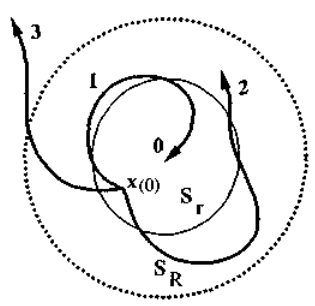
\includegraphics[width=0.3\linewidth]{figure/nonlinear/stable.png}
      \captionof{figure}{稳定与不稳定的示例}
    \end{center}
    \item 考虑如下范德坡(Van der Pol)方程\[\begin{cases}
      \dot{x}_{1}=x_{2}\\\dot{x}_{2}=- x_{1}+(1-{x_{1}}^{2})x_{2}
    \end{cases}\]
    原点是其平衡点。绘出其相轨迹,发现自任意非零状态出发的状态均会趋于一{\bf 极限环(limit cycle)}。\index{极限环(limit cycle)}因此,在极限环内任取一球域,则可见自任意接近原点(也即起始状态的球域半径任意小)的状态出发的轨线最终均会超出该球域而到达极限环,则原点不稳定。此例说明,对于非线性系统,不稳定的形式有多种,未必是线性系统中更常见的“发散至无穷远处”。
    \begin{center}
      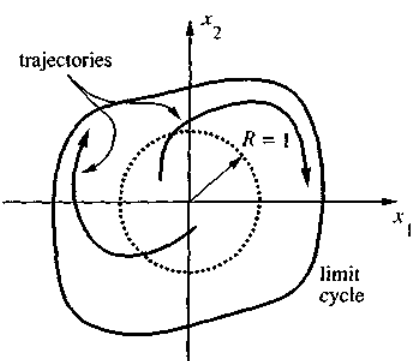
\includegraphics[width=0.34\linewidth]{figure/nonlinear/vanderpol.png}
      \captionof{figure}{范德坡方程的相轨迹}
    \end{center}
    \item 在下图所示的系统中,所有自单位球内非零初始状态出发的轨线,均会先向外到达$C$后再收敛回原点。因此,起始状态无论距离原点多近,解总会超出单位球域,即原点是不稳定的。然而,当时间足够长时,从单位球域内出发的状态总会趋于$0$,即收敛于原点。这也是在渐近稳定性的定义中需要首先以稳定为前提的原因。{\it 称这种轨迹不稳定是合理的,因为类似图中$C$这样的曲线可能已经位于模型可用范围之外。例如,飞机在亚音速和超音速情形下的动力学完全不同。假若我们按亚音速动力学模型绘制出下面相图,那么$C$可能已经进入超音速区域,那么达到$C$的轨线就不再可用。}
    \begin{center}
      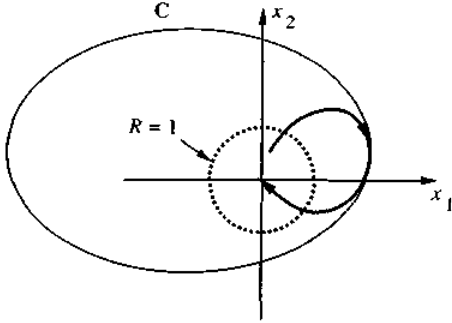
\includegraphics[width=0.35\linewidth]{figure/nonlinear/unstable.png}
      \captionof{figure}{具有收敛性但不稳定的例子之一}
    \end{center}
    \item 考虑系统方程\[\begin{cases}
      \dot{x}=f(x)+y\\\dot{y}=-x
    \end{cases}\]
    其中\[
      f(x)=\begin{cases}-4x,&x>0\\2x,&-1\le x\le 0\\-x-3,&x<-1
    \end{cases}\]
    可分三段求出系统的通解为
    \begin{align*}
      &\begin{cases}x=C_{1}(2-\sqrt{3})\mathrm{e}^{(-2+\sqrt{3})t}+C_{2}(2+\sqrt{3})\mathrm{e}^{(-2-\sqrt{3})t}\\
        y=C_{1}\mathrm{e}^{(-2+\sqrt{3})t}+C_{2}\mathrm{e}^{(-2-\sqrt{3})t}\end{cases}&(x>0)\\
      &\begin{cases}x=C_{1}\mathrm{e}^{t}+C_{2}t\mathrm{e}^{t}\\
        y=(-C_{1}+C_2)\mathrm{e}^{t}-C_{2}t\mathrm{e}^{t}\end{cases}&(-1\le x\le 0)\\
      &\begin{cases}x=\frac{1}{2}\mathrm{e}^{-\frac{t}{2}} C_{1}\Big(\cos\frac{\sqrt{3}}{2}t + \sqrt{3} \sin\frac{\sqrt{3}}{2}t\Big)
        +\frac12\mathrm{e}^{-\frac t2} C_2\Big(\sin\frac{\sqrt{3}}2t-\sqrt{3}\cos\frac{\sqrt{3}}2t\Big) \\
        y=C_{1}\mathrm{e}^{-\frac{t}{2}}\mathrm{cos}\frac{\sqrt{3}}{2}t+C_{2}\mathrm{e}^{-\frac{t}{2}}\mathrm{sin}\frac{\sqrt{3}}{2}t+3 \end{cases}&(x<-1)
    \end{align*}
    根据上面的解绘制出相轨迹如下,可知此系统不稳定,但所有解均会趋于原点。
    \begin{center}
      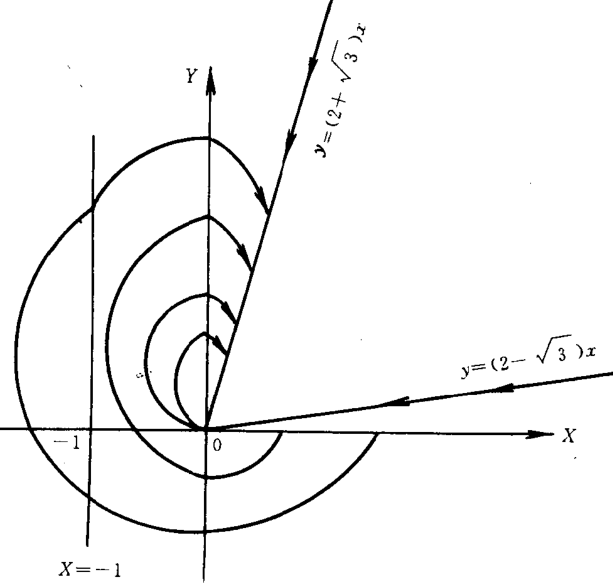
\includegraphics[width=0.4\linewidth]{figure/nonlinear/unstable2.png}
      \captionof{figure}{具有收敛性但不稳定的例子之二}
    \end{center}
  \end{itemize}
\end{example}

\begin{example}[稳定与不稳定的计算例]
  以下两例中$x=0$均为平衡点。\begin{itemize}[leftmargin=1em]
    \item 考虑方程$$\dot{x}=-(1+\sin^2x)x$$
其解为$x(t)=x(0)\mathrm{e}^{-\int_{0}^{t}(1+\sin^{2}x(\tau))\diff\tau}\Rightarrow\|x(t)\|\leq\|x(0)\|\mathrm{e}^{-t}.$
因此,状态$x$指数收敛至$x=0$(其中$\lambda=1$)。
\item 考虑方程$$\dot{x}=-x^2,x(0)=1$$
其解为 $x(t)=\frac1{t+1}$,则$x=0$为渐近稳定的,但不是指数稳定的。
  \end{itemize}
\end{example}

% \input{Chapter_2/Exercises_2A.tex}
% \newpage
\section{正定函数(能量函数)}\label{2Bref}
\begin{definition}[正定、正半定、负定、负半定函数]
  称一函数$V:D\to\R$是\begin{itemize}[leftmargin=1em]
    \item {\bf 正定的(positive definite)},若$V(0)=0$且对任意$x\ne 0$均有$V(x)>0$;\index{正定(positive definite)}
    \item {\bf 正半定的(positive semidefinite)},若$V(0)=0$且对任意$x\ne 0$均有$V(x)\ge0$;\index{正半定(positive semidefinite)}
    \item {\bf 负定的(negative definite)}/{\bf 负半定的(negative semidefinite)},若$-V(x)$是正定/正半定的。\index{负定的(negative definite)}\index{负半定的(negative semidefinite)}
  \end{itemize}
\end{definition}
\begin{note}
  需要特别注意,上面这些函数的输出均为标量,且在$0$处取值均为$0$。
\end{note}
\begin{example}[正定、正半定函数]
  令$x=(x_1,x_2)^\mathrm{T}$。那么
  \begin{itemize}[leftmargin=1em]
    \item $V(x)=x_1^2$是正半定的,因为其在原点处取值为$0$,对于所有$x$均为非负,且对所有满足$x_1=0$($x_2$可为任意值)的$x$均等于$0$。
    \item $V(x)=x_1^2+x_2^2$是正定的,因为其在(且仅在)原点处取值为$0$,对于所有$x$均为非负。
    \item $V(x)=x_1^2+x_2^2+1$不符合正定的定义,因为其在原点处取值不为$0$。
    \item $V(x)=\frac{x_1^2}{1+x_1^2}+x_2^2$是正定的,理由同第二例。
    \item $V(x)=(x_1^2,x_2^2)^\mathrm{T}$不符合正定的定义,因为它的输出不是标量。
  \end{itemize}
\end{example}

\begin{example}[局部正定函数]
  考虑$V(x)=x^2(4-x^2)$($x$为标量),若规定$x\in(-2,2)$,则该函数是正定的;若$x\in[-2,2]$,则该函数是正半定的;对于其余情形,原函数不定。
\end{example}

下面以一个物理系统说明正定函数的物理含义。
\begin{example}[正定函数与能量]\label{pendulum}
  考虑右图所示的含阻尼单摆系统,根据物理知识可写出其动力学方程(注意阻力与速度$l\dot{\theta}$成正比且反向)
  \[lm\ddot{\theta}=-kl\dot{\theta}-mg\sin\theta\]

  \begin{wrapfigure}{R}{0.18\textwidth}
  	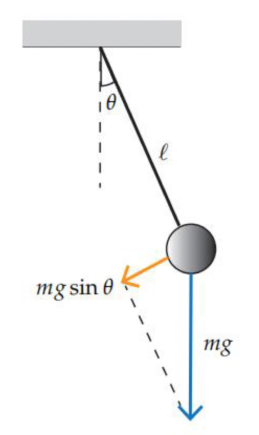
\includegraphics[width=\linewidth]{./figure/nonlinear/pendulum.png}
    \captionof{figure}{带阻尼单摆系统}
  \end{wrapfigure}

  定义$x=(\theta,\dot{\theta})^\mathrm{T}$(限制$-\pi<\theta\le \pi$),那么可写出其状态空间表达式
  \begin{align*}
    \dot{x}_1&=x_2\\
    \dot{x}_2&=-\frac{k}{m}x_2-\frac{g}{l}\sin x_1
  \end{align*}
  
  根据物理中的动能和势能(选最低点为零势能面),写出其总能量\begin{align*}
    V&=\frac{1}{2}mv^2+mgh\\
    &=\frac{1}{2}m(l\dot{\theta})^2+mgl(1-\cos\theta)\\
    &=\frac{1}{2}m(lx_2)^2+mgl(1-\cos x_1)
  \end{align*}

  可见$V$是正定的。求其对$t$的导数可得\begin{align*}
    \dot{V}&=ml^2x_2\dot{x}_2+mgl(\sin x_1)\dot{x}_1\\
    &=ml^2x_2\left(-\frac{k}{m}x_2-\frac{g}{l}\sin x_1\right)+mgl(\sin x_1)x_2\\
    &=-kl^2x_2^2\le0
  \end{align*}

  可见$\dot{V}$是负半定的,意即系统的能量随时间而衰减——这同系统有阻尼相合。
  本例说明,正定函数可看作对于系统内存储的“能量”的数学抽象。之后我们会看到,所有的Lyapunov稳定性定理
  都聚焦于沿系统状态变动的正定函数及其随时间的导数。
\end{example}

最简单也是最为常见的正定函数是{\bf 二次型(quadratic form)}\index{二次型(quadratic form)},其为自$\R{}^n$至$\R{}$的函数\[V(x)=x^\mathrm{T}Px\]其中$P=P^\mathrm{T}\in\R{}^{n\times n}$。二次型函数$V(x)$的正定/正半定/负定/负半定性,取决于$P$的正定/正半定/负定/负半定性。
下面定理证明略去,可参看本科线性代数教材。
\begin{theorem}[实对称矩阵正定、正半定、负定、负半定的判据]\label{pd_nd_thm}
  矩阵$P=P^\mathrm{T}\in\R{}^{n\times n}$是\begin{itemize}[leftmargin=1em]
    \item 正定的,当且仅当其全部特征值都为正,或其所有顺序主子式(矩阵的$i$阶顺序主子式,系矩阵的前$i$行前$i$列这一子块的行列式)均为正;
    \item 正半定的,当且仅当其全部特征值都非负,或其所有主子式(矩阵的$i$阶主子式,系选取$i$行,再以这些行的行号作为列号,取出这些行中对应列的元素,再按原方位排列所构成的$i$阶行列式)均为非负;
    \item 负定的,当且仅当其全部特征值都为负,或其奇数阶顺序主子式为负,偶数阶顺序主子式为正。
    \item 负半定的,当且仅当其全部特征值都非正,或其所有主子式均为非正。
  \end{itemize}
\end{theorem}
\begin{definition}[相似与合同]
  \begin{itemize}[leftmargin=1em]
    \item 称两矩阵$A,B$相似,若存在可逆阵$S$使得$S^{-1}AS=B$;
    \item 称两矩阵$A,B$合同,若存在可逆阵$S$使得$S^{\mathrm{T}}AS=B$。
  \end{itemize}
\end{definition}
\begin{theorem}[实对称矩阵的正交相似对角化]\label{ortho_sim_diag}
  对于任意$P=P^\mathrm{T}\in\R{}^{n\times n}$,均存在一正交矩阵$U$(即$U^\mathrm{T}U=I$)使得$U^{-1}PU=\Lambda$(也即$U^{\mathrm{T}}PU=\Lambda$),
  其中$\Lambda$为对角矩阵,且其对角线上的元素为$P$的所有特征值(均为实数,各特征值出现次数等于代数重数)。
\end{theorem}
注意下述定理无需附加实对称的前提,因为$C^\mathrm{T}C$一定是对称的。
\begin{theorem}[正定、正半定矩阵的分解]\label{pd_npd_div}
  矩阵$P\in\R{}^{n\times n}$是正半定的,当且仅当存在一矩阵$C\in\R{}^{n\times n}$,使得$P=C^\mathrm{T}C$;
  进一步地,$P$是正定的当且仅当$C$可逆(或称为合同于单位阵)。进而,正定矩阵彼此合同。
\end{theorem}
\begin{theorem}[Rayleigh-Ritz不等式]\label{rayleigh-ritz}
  设$P=P^{\mathrm{T}}\in\mathbb{R}^{n\times n}$,并设$\lambda_\mathrm{max}$和$\lambda_\mathrm{min}$分别是$P$的最大特征值和最小特征值。则有
\[\lambda_{\mathrm{min}}\|x\|_{2}^{2}\le x^{\mathrm{T}}Px\le \lambda_{\mathrm{max}}\|x\|_{2}^{2}\]
\end{theorem}
证明可见\href{https://oliverwu.top/file/rayleigh-ritz.pdf}{链接}。
% \input{Chapter_2/Exercises_2B.tex}
% \newpage
\section{自治系统的稳定性定理}\label{2Cref}
\begin{theorem}[Lyapunov稳定性定理]\label{lyapunov}\index{Lyapunov稳定性定理}
  令$x=0$为 \eqref{freeofauto} 的平衡点,$D\subset\R{}^n$为包含$x=0$的域。令$V:D\to\R$为连续可微函数且满足
    \begin{equation}\label{VPD}
      V(0)=0,V(x)>0,\forall x\in D\backslash\{0\}
    \end{equation}
    \begin{equation}\label{VdotNSD}
      \dot{V}(x)\le 0,\forall x\in D
    \end{equation}
  即$V$为正定且$\dot{V}$为负半定,则$x=0$是稳定的。满足上述条件的$V$称为{\bf Lyapunov函数}\index{Lyapunov函数}。
  
  进一步地,若\begin{equation}\label{VdotND}
    \dot{V}(x)< 0,\forall x\in D\backslash\{0\}
  \end{equation}即$\dot{V}$为负定,那么$x=0$是渐近稳定的。
\end{theorem}

\begin{figure}[htbp]
  \centering
  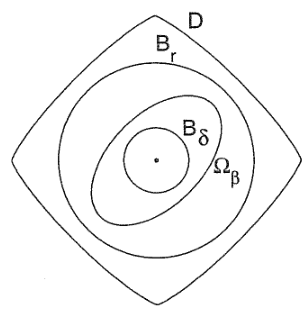
\includegraphics[scale=0.55]{figure/nonlinear/lyapunov-proof.png}
  \caption{定理 \ref{lyapunov} 的证明过程图示}
  \label{lyapunov_proof}
\end{figure}
\newpage
\begin{proof}
  对于$\varepsilon>0$,选取$r\in (0,\varepsilon]$使得\[B_r=\{x\in\R{}^n:\|x\|\le r\}\subset D\]
  令$\alpha=\min\limits_{\|x\|=r}V(x)$\footnote{有界闭集(紧集)上的连续函数必取得最值。},则由 \eqref{VPD} 得$\alpha>0$。取$\beta\in(0,\alpha)$并令\[\Omega_\beta=\{x\in B_r:V(x)\le \beta\}\]
  那么$\Omega_\beta$一定在$B_r$的内部(见图 \ref{lyapunov_proof})\footnote{可用反证法说明。假若$\Omega_\beta$不在$B_r$的内部,则必存在一点$p\in\Omega_\beta$处于$B_r$的边界上。此点处,$V(p)\ge\alpha>\beta$,然而根据$\Omega_\beta$的构成可知对于任意$x\in\Omega_\beta$均有$V(x)\le\beta$,这就产生了矛盾。}。
  若一状态轨线于$t=0$从$\Omega_\beta$中出发,则该轨线一定在所有时刻$t\ge 0$都留在$\Omega_\beta$内部,这是因为由式 \eqref{VdotNSD} 可得
  \[\dot{V}(x(t))\le 0\implies V(x(t))\le V(x(0))\le \beta,\forall t\ge 0\]
  由于$\Omega_\beta$是紧的(这是因为其封闭并以$B_r$为界),那么由定理 \ref{uniqsol},\eqref{freeofauto} 对于所有$t\ge 0$与所有初始状态$x(0)\in\Omega_\beta$均存在唯一解。由于$V(x)$是连续的,且$V(0)=0$,因此存在$\delta>0$使得\[\|x\|\le\delta\implies V(x)<\beta\]
  那么\[B_\delta\subset\Omega_\beta\subset B_r\]且\[x(0)\in B_\delta\implies x(0)\in\Omega_\beta\implies x(t)\in\Omega_\beta\implies x(t)\in B_r\]
  因此\[\|x(0)\|<\delta\implies \|x(t)\|<r\le\varepsilon,\forall t\ge 0\]
  这就说明平衡点$x=0$是稳定的。

  现在假设 \eqref{VdotND} 成立。为证明渐近稳定性,需证明$t\to\infty$时$x(t)\to 0$,也就是证明对于每个$a>0$,均存在一$T>0$使得$\|x(t)\|<a,\forall t>T$。类似上面论述可得对于每个$a>0$,均存在$b>0$使得$\Omega_b\subset B_a$。因此,只需证明$t\to\infty$时$V(x(t))\to 0$即可\footnote{取任意的$a>0$,那么其中总存在$\Omega_b\subset B_a$。若证明了$t\to\infty$时$V(x(t))\to 0$,那么对于任意$b>0$均存在$T$使得$V(x(t))<b,\forall t>T$,也即时间足够长时总有$x(t)\in\Omega_b$,也就是$x(t)\in B_a$,即$\|x(t)\|<a,\forall t>T$。}。
  因为$V(x(t))$单调递减且有下界$0$,因此\[V(x(t))\to c\ge 0,t\to\infty\]
  为证明$c=0$,用反证法。假设$c\ne 0$。由于$V(x)$的连续性,存在$d>0$使得$B_d\subset\Omega_c$。$V(x(t))\to c> 0$意味着对于所有$t\ge 0$,$x(t)$均在球$B_d$外。令$-\gamma=\max\limits_{d\le\|x\|\le r}\dot{V}(x)$(其存在性之缘由同脚注1)。由 \eqref{VdotND} 可得$-\gamma<0$。因此\[V(x(t))=V(x(0))+\int_{0}^{t}\dot{V}(x(\tau))\diff\tau\le V(x(0))-\gamma t\]
  当$t$足够大时,上式右侧将一定变为负值,这和$c>0$的假设矛盾。
\end{proof}

需要特别注意,上述定理仅是充分的。下面用一实例说明。上述定理的推广见下一节。
\enlargethispage{1em}
\begin{example}[利用Lyapunov稳定性定理判别单摆系统稳定性]\label{suff_lyapunov}
  考虑例 \ref{pendulum} 所示的单摆系统。假设其不带阻尼,则其状态方程改写为
  \begin{equation}\label{nodamp}
    \begin{aligned}
      \dot{x}_1&=x_2\\
      \dot{x}_2&=-a\sin x_1
    \end{aligned}
  \end{equation}
  其中$a=g/l>0$。$x=0$为其平衡点,下面研究其稳定性。

  类似例 \ref{pendulum},我们很自然想到,选取其物理意义上的能量函数作为候选Lyapunov函数(Lyapunov function candidate):
  \begin{align*}
    V&=\frac{1}{2}m(lx_2)^2+mgl(1-\cos x_1)\\
    &=ml^2\left(\frac{1}{2}x_2^2+a(1-\cos x_1)\right)
  \end{align*}
  因子$ml^2>0$,不影响$V$的符号,则不妨定义Lyapunov函数为\begin{equation}\label{pendulum_candidate}
  V(x)=\frac{1}{2}x_2^2+a(1-\cos x_1)
\end{equation}
容易看出$V(0)=0$且$V(x)>0,-\pi<x_1<\pi,x_1\ne 0$。求其对$t$的导数可得\begin{align*}
  \dot{V}&=x_2\dot{x}_2+a(\sin x_1)\dot{x}_1\\
  &=a(\sin x_1){x}_2+x_2(-a\sin x_1)=0
\end{align*}
因此原点是稳定的,并且不是渐近稳定的。系统无阻尼,则单摆会一直保持摆动,$x_2$不会趋于$0$,故此论断是合理的。

再考虑有阻尼情形。此时状态方程改写为
  \begin{equation}\label{damped}
    \begin{aligned}
      \dot{x}_1&=x_2\\
      \dot{x}_2&=-a\sin x_1-bx_2
    \end{aligned}
  \end{equation}
其中$b=k/m$。
选取Lyapunov函数如式 \eqref{pendulum_candidate},类似例 \ref{pendulum} 对$t$求导可得$\dot{V}=-bx_2^2\le 0$,
其为负半定,因此我们只能得出原点稳定的结论。然而,原点实际上是渐近稳定的——从物理意义上考虑,有阻尼意味着单摆的摆动幅度会衰减,直至$t\to\infty$时停在最低点($\theta=0,\dot{\theta}=0$)。

事实上,这并不是定理 \ref{lyapunov} 出了问题,而是我们构造的Lyapunov函数不够“好”。我们基于式 \eqref{pendulum_candidate} 进行改造。
将$\frac12x_2^2$换成更加一般的二次型的形式$\frac12x^\mathrm{T}Px$,其中$P$为正定矩阵。则
\begin{align*}
  V&=\frac{1}{2}x^\mathrm{T}Px+a(1-\cos x_1)\\
  &=\frac{1}{2}\begin{bmatrix}
  x_1&x_2
  \end{bmatrix}\begin{bmatrix}
    p_{11}&p_{12}\\p_{12}&p_{22}
    \end{bmatrix}\begin{bmatrix}
      x_1\\x_2
      \end{bmatrix}+a(1-\cos x_1)
\end{align*}
其中$p_{11}>0,p_{11}p_{22}-p_{12}^2>0$。求其对$t$的导数可得\begin{align*}
  \dot{V}&=2\times \frac{1}{2}\begin{bmatrix}
    x_1&x_2
    \end{bmatrix}\begin{bmatrix}
      p_{11}\dot{x}_1+p_{12}\dot{x}_2\\p_{12}\dot{x}_1+p_{22}\dot{x}_2
      \end{bmatrix}+a(\sin x_1)\dot{x}_1\\
    &=\left(p_{11}\dot{x}_1x_1+p_{12}\dot{x}_2x_1+p_{12}\dot{x}_1x_2+p_{22}\dot{x}_2x_2\right)
        +a(\sin x_1)\dot{x}_1\\
      &=p_{11}x_1x_2+p_{12}x_1(-a\sin x_1-bx_2)+p_{12}x_2^2+p_{22}x_2(-a\sin x_1-bx_2)
      +a(\sin x_1)x_2\\
    &=(p_{11}-bp_{12})x_1x_2-p_{12}ax_1\sin x_1-(p_{22}b-p_{12})x_2^2+(1-p_{22})a(\sin x_1)x_2
\end{align*}
观察到(除去系数)第一项不定,第二项为正(注意$x_1\in(-\pi,\pi)$),第三项为正,第四项不定。
则只要让第一、第四项前系数为0,第二、第三项前系数为负即可使其负定。
则\[p_{11}-bp_{12}=0,p_{12}>0,p_{22}b-p_{12}>0,p_{22}=1\]
进而$p_{12}<b$,不妨取为$\frac{b}{2}$,此时$p_{11}=\frac{b^2}{2}>0$,则$p_{11}p_{22}-p_{12}^2=\frac{b^2}{2}-\frac{b^2}{4}>0$,验证得$P$仍为正定。这样得到
\begin{align*}
  \dot{V}=-\frac{1}{2}abx_1\sin x_1-\frac{1}{2}bx_2^2
\end{align*}
可得仅在原点为$0$,其余各处取值均为负,因此其为负定,进而由定理 \ref{lyapunov} 可得原点是渐近稳定的。

本例说明,当我们构造出的Lyapunov函数不适用渐近稳定条件时,不一定表明原系统就非渐近稳定,即定理 \ref{lyapunov} 仅是充分的,通俗地说,它可用于判别一系统{\bf 是}稳定或渐近稳定,但一般无法用于判别一系统{\bf 不是}稳定或渐近稳定。
\end{example}
\begin{example}[局部渐近稳定]
  考虑如下非线性系统\[\begin{aligned}\dot{x}_1&=x_1(x_1^2+x_2^2-2)-4x_1x_2^2\\\dot{x}_2&=x_2(x_1^2+x_2^2-2)+4x_1^2x_2\end{aligned}\]
  原点为其平衡点。构造如下正定函数\[V=\frac{1}{2}(x_1^2+x_2^2)\]
  求其对时间的导数得\[\begin{aligned}
    \dot{V}& =x_{1}\dot{x}_{1}+x_{2}\dot{x}_{2} \\
    &=x_{1}[x_{1}(x_{1}^{2}+x_{2}^{2}-2)-4x_{1}x_{2}^{2}]+x_{2}[x_{2}(x_{1}^{2}+x_{2}^{2}-2)+4x_{1}^{2}x_{2}] \\
    &=(x_1^2+x_2^2)(x_1^2+x_2^2-2)
    \end{aligned}\]
  在球域$B_r=\{x:x_1^2+x_2^2<2\}$内,$\dot{V}$是负定的。

  那么,原点是局部渐近稳定的。
\end{example}
我们“贪心地”希望渐近稳定对于大范围的初始条件都成立,而不是仅像上面例子那样对局部成立。
从定理 \ref{lyapunov} 的证明中可看出,若所有$x\in\mathbf{R}^n$都能找到一有界集合$\Omega_c$以包含之,则定理对全局成立。
这不仅需要$V$的定义域$D=\mathbf{R}^n$,还需要保持$\Omega_c$有界。而这需要对$V$作出进一步的要求。
下面的例子见于前言中参考文献1的123页和文献2的65页。

\begin{example}[径向有界]
  考虑\[V(x)=\frac{x_1^2}{1+x_1^2}+x_2^2\]
  取定$x_2=0$,当$x_1\to\infty$时,该函数趋于$1$,即其对于$x_1$而言是有界的。绘出其等值线如下图。
\begin{center}
  % 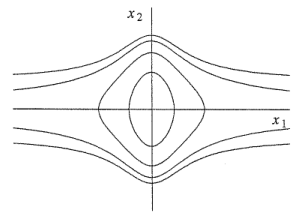
\includegraphics[scale=0.8]{figure/nonlinear/radially.png}
  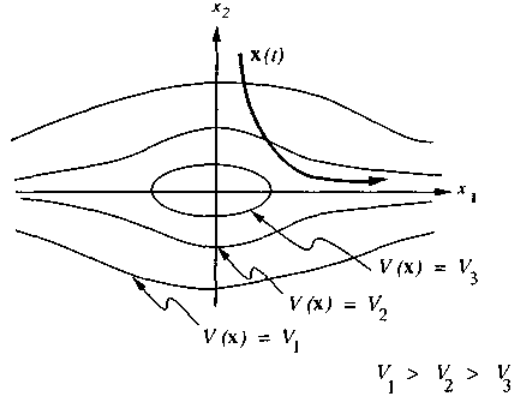
\includegraphics[scale=0.5]{figure/nonlinear/descent_but_unstable.png}
  \captionof{figure}{$V(x)=\frac{x_1^2}{1+x_1^2}+x_2^2$的等值线}
\end{center}
  对于较小的$c$,$V(x)=c$是闭合的,因此$\Omega_c$是有界的,如$\dot{V}<0$,则取一球域$B_r$包含之,即可同 \ref{lyapunov} 之证明找到球域$B_\delta$,使由其中出发的轨线都是渐近稳定的;
  随$c$增长,$V(x)=c$不再闭合,$\Omega_c$无界,则部分状态无法限制于有界$\Omega_c$,如图,从这类状态出发的轨线有可能沿着$V$下降的方向前往无穷远处!
\end{example}
可见,增加径向无界的要求,可能使定理 \ref{lyapunov} 对全局成立。
下述定理印证了这一想法。
\begin{theorem}[全局渐近稳定定理]
  设$V:\R{}^n\to\R$为连续可微函数,且满足
    \begin{itemize}[leftmargin=1em]
      \item $V(0)=0,V(x)>0,\forall x\in \R{}^n\backslash\{0\}$($V$为正定)
      \item $\dot{V}(x)< 0,\forall x\in \R{}^n$($\dot{V}$为负定)
      \item $\|x\|\to\infty\implies V(x)\to \infty$($V$为径向无界,或称为无限大)
    \end{itemize}
  则系统 \eqref{freeofauto} 的平衡点$x=0$是全局渐近稳定的。
\end{theorem}
\begin{proof}
  给定任意点$p\in\R{}^n$,令$c=V(p)$。径向无界条件意味着对任意$c>0$,都存在$r>0$使得$V(x)>c$对任意$\|x\|>r$成立。
  于是$\Omega_c\subset B_r$,则$\Omega_c$是有界的。剩余证明类似定理 \ref{lyapunov}。
\end{proof}
上述定理是下述定理的特例。
\begin{theorem}[Barbashin-Krasovskii定理]\index{Barbashin-Krasovskii定理}
  设$V:\R{}^n\to\R$为连续可微函数,且满足
    \begin{itemize}[leftmargin=1em]
      \item $V(0)=0,V(x)>0,\forall x\in \R{}^n\backslash\{0\}$($V$为正定)
      \item $\dot{V}(x)\le 0,\forall x\in \R{}^n$($\dot{V}$为负半定)
      \item 除零平衡点外,$\dot{V}=0$不包含系统任何整轨线
      \item $\|x\|\to\infty\implies V(x)\to \infty$($V$为径向无界,或称为无限大)
    \end{itemize}
  则系统 \eqref{freeofauto} 的平衡点$x=0$是全局稳定的。
\end{theorem}
具体证明过程略去,可参见前言中的参考文献3的2.3节。
上述定理是对定理 \ref{lyapunov} 的推广,放宽了导数负定的要求。

关于不稳定的判别,有下面定理。
\begin{theorem}[不稳定性判别定理]\label{unstable}
  对于系统 \eqref{freeofauto},若存在函数$V$,它在原点的任意邻域内是正定的,同时$\dot{V}$也是正定的,则系统的平衡点是不稳定的。
\end{theorem}
\section{不变集原理}\label{2Dref}
我们总更希望一个系统是渐近稳定而不仅仅是稳定的。然而,如例 \ref{suff_lyapunov} 所示,我们构造的Lyapunov函数之导数常常只能是负半定而非负定的,从而无法得出渐近稳定的结论。下面将给出Lyapunov稳定性定理的一个推广,它有助于解决此问题。首先介绍相关概念。
\begin{definition}[不变集(invariant set)]\index{不变集(invariant set)}
	称集合$M$是关于式 \eqref{freeofauto} 的{\bf 正不变集(positively invariant set)},
	若\[x(0)\in M\implies x(t)\in M,\forall t\ge0\]
	换言之,每个自$M$内出发的状态轨线,必整体留在$M$内。
\end{definition}
\begin{definition}[趋于集合(approach a set)]
	称$t\to\infty$时,$x(t)$趋于一集合$M$,若\[\forall \varepsilon>0,\exists T>0:\operatorname{dist}(x(t),M)<\varepsilon,\forall t>T\]
	其中$\operatorname{dist}(p,M)=\inf\limits_{x\in M}\|p-x\|$。换言之,时间足够长时,$x(t)$与$M$的“距离最小值”将趋于0。
\end{definition}
\begin{example}[不变集]\label{invset}
	\begin{itemize}[leftmargin=1em]
		\item 平衡点
		\item $\R{}^n$
		\item $\Omega_c=\{x\in\R{}^n:V(x)\le c\}$,其中$\dot{V}(x)\le 0$。此不变集之后很常用到。
		\item 极限环\index{极限环(limit cycle)}:称一状态轨线是封闭的,若其非常值,且存在$t_0>0$,使得$x(t+t_0)=x(t)$(总会复归之前的状态)。称一孤立的封闭状态轨线为极限环。例子可见 \ref{stable_unstable}。其类别有
		\begin{itemize}[leftmargin=1em]
			\item 稳定极限环:极限环附近的所有轨迹皆收敛于它($t\to\infty$)
			\item 不稳定极限环:极限环附近的所有轨迹皆不收敛于它($t\to\infty$)
			\item 半稳定极限环:极限环附近的轨迹,部分收敛于它,另一部分发散($t\to\infty$)
		\end{itemize}
	\end{itemize}
\end{example}
有了上面的铺垫,我们不加证明地给出下述定理。
\begin{theorem}[LaSalle不变集原理]\label{lasalle}\index{LaSalle不变集原理}
	对于系统 \eqref{freeofauto},设\begin{itemize}[leftmargin=1em]
		\item $\Omega\subset D$为紧的正不变集;
		\item $V:D\to\R{}$是连续可微函数,且在$\Omega$中满足$\dot{V}(x)\le 0$;
		\item $E=\{x\in\Omega: \dot{V}(x)= 0\}$;
		\item $M$为$E$中最大的不变集。
	\end{itemize}
	那么当$t\to\infty$,每个自$\Omega$中出发的轨线都将趋于$M$。
\end{theorem}
\begin{note}
	不变集可视为平衡点的推广。注意,$V$并不需要是正定函数。
\end{note}
\begin{corollary}
	令$x=0$为 \eqref{freeofauto} 的平衡点。$D\in\R{}^n$是包含原点的域。令$V:D\to\R{}$是$C^1$正定函数,且$\dot{V}\le 0$在$D$上总成立。
	令$E=\{x\in D:\dot{V}=0\}$,并设除了平凡解$x(t)=0$外,没有解能一直处于$E$中。那么$x=0$是渐近稳定的。
\end{corollary}
\begin{corollary}\label{lasallegas}
	令$x=0$为 \eqref{freeofauto} 的平衡点。令$V:\R{}^n\to\R{}$是径向无界的$C^1$正定函数,且$\dot{V}\le 0$在$\R{}^n$上总成立。
	令$E=\{x\in \R{}^n:\dot{V}=0\}$,并设除了平凡解$x(t)=0$外,没有解能一直处于$E$中。那么$x=0$是全局渐近稳定的。
\end{corollary}
\begin{note}
	在$\dot{V}$负定时,$E=\{0\}$,上述推论即退化为 \ref{lyapunov}。
\end{note}
\begin{example}[利用LaSalle定理判别单摆系统稳定性]
	考虑例 \ref{suff_lyapunov}。首先考虑无阻尼的情形 \eqref{nodamp},Lyapunov函数\[V(x)=\frac{1}{2}x_2^2+a(1-\cos x_1)\]
	可构造不变集$\Omega$类似例 \ref{invset} 第三点(不过需注意定义域):\[\Omega=\{x:V(x)\le c\},c>0\]
	例 \ref{suff_lyapunov} 已经计算过$\dot{V}=0$,因此$E=\Omega$。
	$E$中最大的不变集$M$,显然就是$\Omega$本身。于是利用 \ref{lasalle},$\Omega$中出发的轨线都将趋于$\Omega$。

	再考虑有阻尼的情形 \eqref{damped}。仍然选择$\Omega$如上。由于$\dot{V}=0\iff x_2=0$,因此\[E=\{x:x_2=0,x\in\Omega\}\]
	再找$E$中最大的不变集。由于自$x_1\ne 0,x_2=0$起始的状态轨线,一经出发,必然使得$x_2\ne 0$(从物理意义上考虑:在非最低点从静止释放单摆,
	单摆必定马上具有非零速度)。因此$M=\{(0,0)\}$。此时利用 \ref{lasalle},可得每个自$\Omega$中出发的轨线都将趋于原点。我们发现,这样也说明了原点的渐近稳定性。
\end{example}
\begin{example}[利用LaSalle定理判别自适应控制的收敛性]
	考虑如下一阶系统
  \[ \dot{y} = a  y + u \]
  对其作用自适应控制律
  \[ u = - k  y, \dot{k} = \gamma y^2, \gamma > 0. \]
  取$x_1 = y, x_2 = k$,我们可得
  \[ \left\{\begin{array}{l}
       \dot{x}_1 = a  x_1 - x_1 x_2\\
       \dot{x}_2 = \gamma x^2_1
     \end{array}\right. \]
  $\{x:x_1 = 0\}$是一个由平衡点构成的集合(将$x_1=0$代入验证即可)。我们想要说明在$t \rightarrow \infty$
  时状态轨线将收敛到这个集合上,从而说明自适应律可使$y$收敛至$0$。
  
  考虑如下函数
  \begin{equation}\label{adaptive_eg_candidate}
	V (x) = \frac{1}{2} x^2_1 + \frac{1}{2} (x_2 - k_0)^2
  \end{equation}
  其中$k_0$为常数,加入此项的缘由是上述平衡点集并没有保证$x_2=0$。注意,这个函数并不是正定的
  (因其在原点取值非零),但是这并不违背LaSalle定理的条件。
  
  $V$随时间的导数为
  \begin{align*}
    \dot{V} & =  x_1 \dot{x}_1 +  (x_2 - k_0) \dot{x}_2\\
    & =  x_1 (a  x_1 - x_1 x_2) + (x_2 - k_0) \gamma x^2_1\\
	&= ax_1^2-x_1^2x_2+\gamma(x_2x_1^2-k_0x_1^2)
  \end{align*}
  我们发现,如果在 \eqref{adaptive_eg_candidate} 第二项中加入$\frac{1}{\gamma}$,那么上式就有可消去的项。则
  \[V (x) = \frac{1}{2} x^2_1 + \frac{1}{2\textcolor{structurecolor}{\gamma}} (x_2 - k_0)^2, \dot{V}  =  (a - k_0)  x^2_1\]
  取 $k_0 > a$,则 $\dot{V} \leq 0$。

  接下来应用LaSalle定理。首先定义不变集$\Omega = \{ x \in \mathbf{R}^2 : V (x) \leq c \},c>0$。
  则集合$E =\{ x \in \Omega :\dot{V}= 0 \}= \{ x \in \Omega : x_1 = 0 \}$。进而由本例开头的分析知$M = E$。
  根据 \ref{lasalle},解会收敛至$x_1=0$上,也即$\lim\limits_{t \rightarrow \infty} x_1 (t) = 0$。
  又知$V(x)$径向无界,所以由 \ref{lasallegas},此结论全局成立。
\end{example}
定理 \ref{lasalle} 除了可用于判别趋于原点的情形,还可推广用于判别收敛至极限环等。
\begin{example}[收敛至极限环]
	考虑下述非线性系统\begin{align*}
		\dot{x}_1&=x_2+x_1(\beta^2-x_1^2-x_2^2)\\
		\dot{x}_2&=-x_1+x_2(\beta^2-x_1^2-x_2^2)
	\end{align*}
	原点是平衡点(通过验证$x_1=x_2=0$时$\dot{x}_1=\dot{x}_2=0$即可)。

	我们又发现,如果$x_1^2+x_2^2=\beta^2$,那么系统方程改写为\[\left\{\begin{array}{l}
    \dot{x}_1 = x_2\\
    \dot{x}_2 = - x_1
  \end{array}\right.\]
  对$x_1^2+x_2^2=\beta^2$求导并将上面的式子代入可发现恒成立(也可通过几何层面,由上述方程也表示圆的方程看出),
  这样一来,自$x_1^2+x_2^2=\beta^2$出发的轨线会一直在其上运动,因此形成了一个极限环,同时也是不变集。

  \begin{note}
    定性分析极限环性质:设$r = \sqrt{x^2_1 + x^2_2}, \theta = \arctan \frac{x_2}{x_1}$,我们有(注意此时应代入原方程)
  \begin{align*}
    \dot{r}& = \frac{1}{2}(x_{1}^{2}+x_{2}^{2})^{-\frac{1}{2}}(2x_{1}\dot{x}_{1}+2x_{2}\dot{x}_{2})= r (\beta^2 - r^2)\\
    \dot{\theta} & =\frac{1}{1+(\frac{x_{2}}{x_{1}})^{2}}\frac{\dot{x}_{2}x_{1}-\dot{x}_{1}x_{2}}{x_{1}^{2}}= - 1
  \end{align*}
  其中用到了
  \begin{align*}
    x_1\dot{x}_1+x_2\dot{x}_2& = (x_1^2+x_2^2)(\beta^2-x_1^2-x_2^2)= r^2 (\beta^2 - r^2)\\
    x_1\dot{x}_2-x_2\dot{x}_1 & = -(x_1^2+x_2^2)=- r^2
  \end{align*}
  则 \ $\left\{\begin{array}{l}
    r < \beta, \dot{r} > 0 \Rightarrow r \rightarrow \beta\\
    r > \beta, \dot{r} < 0 \Rightarrow r \rightarrow \beta
  \end{array}\right. \Rightarrow$ 极限环稳定。
\end{note}

  下面利用LaSalle定理来分析。构造如下候选Lyapunov函数\[ V (x) = \frac{1}{4} (x^2_1 + x^2_2 - \beta^2)^2 \]
  构造此函数的动机是,它衡量了与极限环的“距离”。显然$V (x) \geq 0$,但要注意同上个例子一样,此函数也不是正定的。求其导数得
  \begin{align*}
    \dot{V} (x) & =  \frac{1}{2} (x^2_1 + x^2_2 - \beta^2) (2 x_1 \dot{x}_1 +
    2 x_2 \dot{x}_2)\\
    & =  - (x^2_1 + x^2_2 - \beta^2)^2 (x^2_1 + x^2_2)\leq 0
  \end{align*}
  构造集合$\Omega_c =
  \{ x \in \mathbf{R}^2 : V (x) \leq c \},c > 0$。因为$\dot{V} \leq 0$,所以这是不变集。
  接下来寻求$E = \{ x \in \Omega_c : \dot{V} (x) = 0 \}$。根据导函数形式可得$E = \{
  (0, 0) \} \cup \{ x : x^2_1 + x^2_2 = \beta^2 \}$。
  不过,要注意这只在$c \ge \frac{1}{4} \beta^4$时成立——因为$0 < c < \frac{1}{4} \beta^4$时,
  $\Omega_c $不包含原点,此时$E=\{ x : x^2_1 + x^2_2 = \beta^2 \}$。
  最后,根据前面所做的分析,$E$中的最大不变集$M = E$。
  
  这样,利用 \ref{lasalle},其中$c \in \left( 0,
  \frac{1}{4} \beta^4 \right)$,即知每个自$\Omega_c$出发的轨线均收敛至极限环,因此极限环稳定。
  取$c=\frac{1}{4} \beta^4-\varepsilon$,其中$\varepsilon$可任意小,我们发现,无限接近于原点的状态也都会收敛至极限环,则原点不稳定。

  \begin{note}
    要判别原点的不稳定性,亦可构造如下候选Lyapunov函数\[V=\frac12(x_1^2+x_2^2)\]
  求导得\begin{align*}
	  \dot{V}&=x_1\dot{x}_1+x_2\dot{x}_2=(x_1^2+x_2^2)(\beta^2-x_1^2-x_2^2)
  \end{align*}
  其在原点的小邻域内为正定,则运用定理 \ref{unstable} 即可。
  \end{note} 
\end{example}

\section{线性系统与线性化}\label{2Eref}
线性系统中,对应于非线性自治系统的是线性定常(线性时不变,Linear Time-Invariant,简写作LTI)系统
\begin{equation}\label{LTI}
    \dot{x}=Ax
\end{equation}

  Lyapunov分析法使我们得以在同一框架下研究线性和非线性系统(将LTI视为非线性系统的一个特例)。
 接下来,我们将引入在文献中经常出现的一类非常有用的Lyapunov函数,再通过状态方程的线性化反过来研究非线性系统的稳定性,并了解此法有何局限性。

  在研究LTI系统 \eqref{LTI} 时,常用下面的二次型作为候选Lyapunov函数
  \[ V (x) = x^\mathrm{T} P  x \]
  其中$P \in \mathbf{R}^{n \times n}$ 为正定。求其导数
  \begin{align*}
    \dot{V}(x)&= x^\mathrm{T}P\dot{x}+\dot{x}^\mathrm{T}Px\\
    &=x^\mathrm{T}PAx+(Ax)^\mathrm{T}Px\\
    &=x^\mathrm{T} (P  A + A^\mathrm{T} P) x \\
    &\triangleq - x^\mathrm{T} Q  x
  \end{align*}
  其中$Q$是定义为
  \begin{equation}
    P  A + A^\mathrm{T} P = - Q \label{lyaLTI}
  \end{equation}
  的对称矩阵。
  若$Q$正定,那么系统 \eqref{LTI} 的原点就是渐近稳定的。

  下面给出LTI系统的稳定性判据。此定理的证明可参看《线性系统理论》相关教材。
  
  \begin{theorem}[线性定常系统的稳定性判据]\label{linearlya}
    系统 \eqref{LTI} 中的原点是渐近稳定的,或$A$是Hurwitz的(意即其所有特征值均具有负实部),当且仅当
    对于任意给定的对称正定矩阵$Q$,都存在唯一的对称正定矩阵$P$使得 \eqref{lyaLTI} 成立。
  \end{theorem}
  \begin{note}
    注意,此判据是充要条件。
  \end{note}
  
  下面利用线性化,将这个结论推广至非线性系统。

  以分析原点的稳定性为例。将系统 \eqref{freeofauto} 在原点附近线性化得\begin{equation}
    \dot{x}=Ax+g(x)
  \end{equation}
  其中
  \begin{equation}\label{jacobian}
    A=\frac{\partial f(x)}{\partial x}|_{x=0}=\left.\begin{bmatrix}\frac{\partial f_{1}}{\partial x_{1}}&\cdots&\frac{\partial f_{n}}{\partial x_{1}}\\\vdots&&\vdots\\\frac{\partial f_{n}}{\partial x_{1}}&\cdots&\frac{\partial f_{n}}{\partial x_{n}}\end{bmatrix}\right|_{x=0}
  \end{equation}
  称为雅可比矩阵(Jacobian)\index{雅可比矩阵(Jacobian)},且有(所用范数均为2-范数)
  \begin{equation}\label{gxto0}
    \|x\|\to0\ \text{时}\ \cfrac{\|g(x)\|}{\|x\|}\to0
  \end{equation}
  考虑候选Lyapunov函数
  \[ V (x) = x^\mathrm{T} P  x \]
  其中$P \in \mathbf{R}^{n \times n}$ 为正定。其导数等于
  \begin{equation}
    \begin{aligned}
    \dot{V}&= x^\mathrm{T}P\dot{x}+\dot{x}^\mathrm{T}Px\\
    &= x^\mathrm{T}P(Ax+g(x))+(Ax+g(x))^\mathrm{T}Px\\
    &= x^\mathrm{T}(PA+A^\mathrm{T}P)x+x^\mathrm{T}Pg(x)+g^\mathrm{T}(x)Px\\
    &=-x^\mathrm{T}Qx+2xPg(x)
    \end{aligned}
  \end{equation}
  其中第四个等号,是由于$x^\mathrm{T}Pg(x)$为标量,所以转置与本身相等,
  而其转置刚好就是最后一项(利用$P$的对称性)。
  
  因为$A$是Hurwitz的,根据 \ref{linearlya} 有$x^\mathrm{T}Qx> 0$。至于另一项,由 \eqref{gxto0},
  对$\forall \gamma>0$,$\exists r>0$使得\[\frac{\|g(x)\|}{\|x\|}\le \gamma,\quad\forall\|x\|\le r\]
  因此$\|x\|\le r$时有\begin{align*}
    \dot{V}&\le -x^\mathrm{T}Qx+2\|x\|\|P\|\|g(x)\|\\
    &\le -x^\mathrm{T}Qx+2\gamma\|x\|^2\|P\|\\
    &\le -\lambda_{\min}(Q)\|x\|^2+2\gamma \|P\|\|x\|^2\\
    &= -(\lambda_{\min}(Q)-2\gamma\|P\|)\|x\|^2
  \end{align*}

  第一个不等号是由于范数相容性,第三个不等号是由Rayleigh-Ritz不等式 \ref{rayleigh-ritz}。
  这样,选$\gamma$使得$\lambda_{\min}(Q)>2\gamma \|P\|$,即可使得$\dot{V}$是负定的。此时$x=0$就是渐近稳定的。

  将上述方法归纳为下面定理。
  \begin{theorem}[通过线性化判别非线性系统稳定性]
    对于系统 \eqref{freeofauto},如果对于式 \eqref{jacobian} 所示雅可比矩阵$A$\index{雅可比矩阵(Jacobian)},有
    \begin{itemize}[leftmargin=1em]
    \item $\forall i, \ensuremath{\operatorname{Re}} [\lambda_i (A)] < 0$,则系统 \eqref{freeofauto} 的原点是渐近稳定的;
    \item $\exists i, \ensuremath{\operatorname{Re}} [\lambda_i (A)] > 0$,则系统 \eqref{freeofauto} 的原点是不稳定的;
    \item $\forall i, \ensuremath{\operatorname{Re}} [\lambda_i (A)] \le 0$,且
    $\exists j, \ensuremath{\operatorname{Re}} [\lambda_j (A)] = 0$,无法判断。
    \end{itemize}
  \end{theorem}
  \begin{note}
    上面定理的直观解释:在平衡点附近线性化,也可看作对所得线性系统施加小扰动。对于所得线性系统特征值严格落在左半平面或右半平面的情形,
    这种扰动不会使得特征值跨越虚轴从而改变系统性质;然而,若所得线性系统存在虚轴上的特征值,则扰动可能使其进入左半平面,也可能
    使其进入右半平面,因此我们无法做出判断。

    由于线性化过程依赖于“平衡点附近”的假设,因此只能得出局部渐近稳定的结论,这也就是此法的局限性。
  \end{note}
  \newpage
  \begin{example}[通过平衡点附近的线性化判别单摆系统的稳定性]
   考虑单摆系统 \eqref{damped}。利用线性化检验$(0, 0)$ 和 $(\pi, 0)$这两个平衡点的稳定性。
    \[ A_1 = \left. \frac{\partial f}{\partial x} \right|_{x = (0, 0)} = \left.
       \left[\begin{array}{cc}
         0 & 1\\
         -a\ensuremath{\operatorname{cos}}  x_1 & - b
       \end{array}\right] \right|_{x = (0, 0)} = \left[\begin{array}{cc}
         0 & 1\\
         - a & - b
       \end{array}\right] \]
    特征方程是 $\lambda^2 + b \lambda + a = 0$,两特征值之和为负、之积为正,则一定都在左半平面。因此该系统在$(0, 0)$附近是稳定的。
    \[ A_2 = \left. \frac{\partial f}{\partial x} \right|_{x = (\pi, 0)} =
       \left. \left[\begin{array}{cc}
         0 & 1\\
         -a\ensuremath{\operatorname{cos}}  x_1 & - b
       \end{array}\right] \right|_{x = (\pi, 0)} = \left[\begin{array}{cc}
         0 & 1\\
         a & - b
       \end{array}\right] \]
       特征方程是 $\lambda^2 + b \lambda - a = 0$,两特征值之积为负,则一定有处于右半平面的特征值。因此该系统在$(\pi, 0)$附近不稳定。
      从物理上考虑则不难理解:$(\pi, 0)$对应的实为单摆竖立最高点(最低点的对称点)。
    \begin{note}
      对于一元二次方程 $a  x^2 + b  x + c = 0$,其解$x_{1},x_{2}$满足韦达定理
      \[ x_1 + x_2 = \frac{- b}{a}, \quad x_1  x_2 = \frac{c}{a} \]
      对于$a = 1$情形,若$c > 0$则两根同号;若还有$b>0$,那么两根均具有负实部。
      同样对于$a = 1$情形,若$c < 0$则两根异号。
    \end{note}
  \end{example}

\chapter{非自治系统的稳定性分析}\label{cp3}

% \newpage
\section{比较函数}\label{3Aref}

\begin{definition}[$\mathcal{K}$ 类函数、 $\mathcal{K}_{\infty}$类函数]
  称连续函数 $\alpha : [0, a) \rightarrow [0, \infty)$ 属于 $\mathcal{K}$ 类,若其严格单调递增且 $\alpha (0) =0$。
  进一步地,称其属于 $\mathcal{K}_{\infty}$类,若 $a = \infty$ 且$r \rightarrow \infty$时
  $\alpha (r) \rightarrow \infty$。
\end{definition}

\begin{definition}[$\mathcal{K}\mathcal{L}$类函数]
  称连续函数 $\beta : [0, a) \times [0, \infty) \rightarrow [0,
  \infty)$ 属于 $\mathcal{K}\mathcal{L}$ 类,若映射$\beta (r, t)$对每个取定的$t$,关于$r$ 属于 $\mathcal{K}$类,
  并且对每个取定的$r$,随着$t
  \rightarrow \infty$,$\beta (r, t)$单调递减并趋于$ 0$。
\end{definition}

\begin{example}  [$\mathcal{K}$ 类、 $\mathcal{K}_{\infty}$类、$\mathcal{K}\mathcal{L}$类函数]
  \begin{itemize}[leftmargin=1em]
    \item $\alpha (r) = \arctan (r)$。由$\alpha' (r) = \frac{1}{r^2 + 1} \geq 0,
    \alpha (0) = 0, \lim\limits_{r \rightarrow \infty} \alpha (r) = \frac{\pi}{2}$,
    所以$\alpha (r)$ 属于 $\mathcal{K}$类,但不属于 $\mathcal{K}_{\infty}$类函数。
    
    \item $\alpha (r) = r^c$。由$ \alpha' (r) = c r^{c-1} \geq 0, \alpha (0) = 0, \lim\limits_{r
    \rightarrow \infty} \alpha (r) = \infty$,所以 $\alpha (r)$ 属于 $\mathcal{K}_{\infty}$类函数。
    
    \item $\alpha (r) = \min \{ r, r^2 \}$ 属于 $\mathcal{K}_{\infty}$类函数。
    
    \item $\beta (r, t) = r^2 e^{- t}$ 属于    $\mathcal{K}\mathcal{L}$类函数。
    \item $\beta (r, t) = \frac{r}{rt+1}=\frac{1}{t+\frac1\gamma}$ 属于 $\mathcal{K}\mathcal{L}$类函数。
  \end{itemize}
\end{example}

\begin{lemma}[$\mathcal{K}$类、$\mathcal{K}_\infty$类、$\mathcal{K}\mathcal{L}$类函数的复合]\label{klcomp}
  设定义在$[0,a)$上的函数$\alpha_{1},\alpha_{2}\in\mathcal{K}$,$\alpha_{3},\alpha_{4}\in\mathcal{K}_{\infty}$且有
  $\beta\in\mathcal{KL}$。令$\alpha_{i}^{-1}$表示$\alpha_{i}$的反函数。则
  \begin{itemize}[leftmargin=1em]
    \item $\alpha_{1}^{-1}$定义在$[0,\alpha_{1}(a))$上,属于$\mathcal{K}$类函数;
    \item $\alpha_{3}^{-1}$定义在$[0,\infty)$上,属于$\mathcal{K}_\infty$类函数;
    \item $\alpha_{1} \circ\alpha_{2}$属于$\mathcal{K}$类函数;
    \item $\alpha_{3} \circ\alpha_{4}$属于$\mathcal{K}_\infty$类函数;
    \item $\sigma(r,t)=\alpha_{1}(\beta(\alpha_{2}(r),t)) $属于$\mathcal{K}\mathcal{L}$类函数。
  \end{itemize}
\end{lemma}

通过下面的引理,我们将$\mathcal{K}$、$\mathcal{K}_\infty$ 和$\mathcal{K}\mathcal{L}$函数引入Lyapunov分析中。

\begin{lemma}\label{lyapunov_comp}
  $V : D \rightarrow \mathbf{R}$ 是连续的正定函数,$D\subset\mathbf{R}^n$是包含原点的域。
  令$B_r\subset D$($r>0$)。那么存在定义在$[0,r]$上的
  $\mathcal{K}$ 类函数$\alpha_1,\alpha_2$使得
  \[ \alpha_1 (\| x \|) \leq V (x) \leq \alpha_2 (\| x \|), \forall x \in B_r \]
  若$D =\mathbf{R}^n$,那么$\alpha_1,\alpha_2$应定义在$[0,\infty)$上。
  进一步,若$V(x)$是径向无界的,那么 $\alpha_1$与 $\alpha_2$可选为 $\mathcal{K}_{\infty}$类函数。
\end{lemma}

\begin{example}
  设$V (x) = x^\mathrm{T} P  x$,$P$正定。由不等式 \ref{rayleigh-ritz},可取上述引理中的$\alpha_1=\lambda_{\min} (P)r^2$,$\alpha_2=\lambda_{\max} (P)r^2$。
\end{example}
为了看出 \ref{lyapunov_comp} 是如何用于Lyapunov分析的,下面利用它来证明定理 \ref{lyapunov}。
在证明中,我们尝试选取$\delta$和$\beta$使得$B_\delta\subset\Omega_\beta\subset B_r$。利用上述引理
我们知道\[\alpha_1 (\| x \|) \leq V (x) \leq \alpha_2 (\| x \|)\]
可取$\beta\le\alpha_1(r)$和$\delta\le\alpha_2^{-1}(\beta)$(即$\alpha_2(\delta)\le\beta$)。首先可得
\[V(x)\le\beta\implies\alpha_1(\|x\|)\le\alpha_1(r)\iff \|x\|\le r\]
其中的等价号是由$\alpha_1$的单调性。这样就得到了$\Omega_\beta\subset B_r$。
还可得\[\|x\|\le\delta\implies V(x)\le\alpha_2(\delta)\le\beta\]
这样就得到了$B_\delta\subset\Omega_\beta$。
关于渐近稳定性的证明,尚需要一些其他的结论,可参考前言中的参考文献1(145-146页)。

下面两个引理也是利用比较函数进行Lyapunov分析的例子,可自行证明之。
\begin{lemma}
  系统 (\ref{freeofauto}) 的平衡点 $x = 0$ 是稳定的,当且仅当存在一$\mathcal{K}$类函数 $\alpha (\cdot)$
  和常数$\delta$ 使得
  \[ \| x (0) \| \leq \delta \quad \Rightarrow \quad \| x (t) \| \leq \alpha
     (\| x (0) \|), \forall t \geq 0. \]
\end{lemma}

\begin{lemma}
  系统 (\ref{freeofauto}) 的平衡点 $x = 0$ 是渐近稳定的,当且仅当存在一
  $\mathcal{K}\mathcal{L}$类函数 $\beta (\cdot,\cdot)$与常数 $\delta$
  使得
  \[ \| x (0) \| \leq \delta \quad \Rightarrow \quad \| x (t) \| \leq \beta
     (\| x (0) \|, t), \forall t \geq 0. \]
\end{lemma}
% \input{Chapter_3/Exercises_3A.tex}
% \newpage
\section{非自治系统稳定性的概念}\label{3Bref}
考虑非自治系统的自由运动
\begin{equation}\label{freeofnonauto}
  \dot{x}=f(t,x)
\end{equation}
其中$f : [0, \infty) \times D \rightarrow \R{}^n$是从$[0, \infty) \times D$至$\R{}^n$的映射,它对$t$分段连续,对$x$局部Lipschitz。$D\subset\R{}^n$为包含$x=0$的域。若$f(t,0)\equiv0,\forall t\ge t_0$,则$x=0$为$t=t_0$时刻的平衡点。
\begin{definition}[非自治系统的稳定性]
 系统 \eqref{freeofnonauto} 的平衡点 $x = 0$是
  \begin{itemize}[leftmargin=1em]
    \item {\bf 稳定的(stable)}\index{稳定的(stable)},若对每个$\varepsilon > 0$,都存在 $\delta =
    \delta (\varepsilon, t_0)$使得
    \begin{equation}
      \| x (t_0) \| < \delta \quad \Rightarrow \quad \| x (t) \| <
      \varepsilon, \forall t \geq t_0 \geq 0 \label{Nonauto:stable:def} .
    \end{equation}
    \item {\bf 不稳定的(unstable)}\index{不稳定的(unstable)},若其不是稳定的。
    
    \item {\bf 一致稳定的(uniformly stable)}\index{稳定的(stable)!一致$\sim$(uniformly)},若对每个$\varepsilon > 0$,都存在
    $\delta = \delta (\varepsilon) > 0$(与$t_0$无关),使得 \eqref{Nonauto:stable:def} 成立。
    
    \item {\bf 渐近稳定的(asymptotically stable)}\index{稳定的(stable)!渐近$\sim$(asymptotically)},若其是稳定的,且存在一正数
     $c = c (t_0)$ 使得
    \begin{equation}
      \forall \| x (t_0) \| < c, \lim_{t \rightarrow \infty} x (t) \rightarrow
      0 \label{Nonauto:astable:def} .
    \end{equation}
    \item {\bf 一致渐近稳定的(uniformly asymptotically stable)},\index{稳定的(stable)!一致渐近$\sim$(uniformly asymptotically)}若其为一致稳定的,且存在一正常数 $c$(与$t_0$无关)使得 \eqref{Nonauto:astable:def} 成立;换言之,对任意$\eta>0$,都存在$T=T(\eta)>0$使
    \[\|x(t)\|<\eta,\forall t\ge t_0+T(\eta),\forall\|x(t_0)\|<c\]
    
    \item {\bf 全局一致渐近稳定的(globally uniformly asymptotically stable)}\index{稳定的(stable)!全局一致渐近$\sim$(globally uniformly asymptotically)},若其是一致稳定的,$\delta(\varepsilon)$满足$\lim\limits_{\varepsilon\to\infty}\delta(\varepsilon)=\infty$,且对于任意正数$\eta$和$c$,都存在$T=T(\eta,c)>0$使得
    \[\|x(t)\|<\eta,\forall t\ge t_0+T(\eta,c),\forall\|x(t_0)\|<c\]
  \end{itemize}
\end{definition}
\begin{note}
  “一致”是说初始时刻任意性,“全局”则是说初始状态任意性。一致渐近稳定,通俗地说,就是只要时间足够长,状态总能进入给定的离原点足够近的范围(渐近),
  并且经过的时间$T$仅与所要求的状态与原点的距离有关($T(\eta)$),而与初始时刻无关(一致);全局一致渐近稳定,则是在此基础上加入了“全局”的要求,也即初始状态任意($c$能取遍所有的正数)。达到与原点给定距离之内的用时$T$,仍然与初始时刻无关,
  不过增加了对初始状态的相关性($T(\eta,c)$)——很容易理解:不能要求“很远”的初始状态与“很近”的初始状态有相同的过渡时间。
\end{note}
下面的引理利用比较函数,给出了一致稳定和一致渐近稳定的更为简洁明了的定义。
\begin{lemma}
  系统 \eqref{freeofnonauto} 的平衡点 $x = 0$是
  \begin{itemize}[leftmargin=1em]
  \item 稳定的,当且仅当存在一$\mathcal{K}$类函数 $\alpha$和常数
  $c$ 使得
   \[ \| x (t) \| \leq \alpha (\| x (t_0) \|), \forall t \geq t_0 \geq 0,
       \forall \| x (t_0) \| \le c. \]
  \item 一致稳定的,当且仅当存在一$\mathcal{K}\mathcal{L}$ 类函数 $\beta$ 和正常数$c$(与$t_0$无关),使得
  \begin{equation}
    \| x (t) \| \leq \beta (\| x (t_0) \|, t - t_0), \forall t \geq t_0 \geq
    0, \forall \| x (t_0) \| \le  c \label{uas:iff:kl} .
  \end{equation}
  \item 全局一致渐近稳定的,若不等式 \eqref{uas:iff:kl} 对所有初始状态$x (t_0)$都成立,即$c$可取至$\infty$。
  \item 一致指数稳定的,若上述$\beta$具有$\beta(r,t)=kr\mathrm{e}^{-\lambda t}$的形式:
  \[\|x(t)\|\le k\|x(t_0)\|\mathrm{e}^{-\lambda(t-t_0)}, \forall t \geq t_0,\forall \| x (t_0) \| \le  c \]
  \end{itemize}
\end{lemma}

\begin{example}[稳定但不一致稳定]
  考虑如下非线性系统
  \[ \dot{x} = (6 t  \sin  t - 2 t) x \]
  其解为
  \begin{align*}
    x (t) & =  x (t_0) \exp \left\{ \int^t_{t_0} (6 \tau \sin \tau - 2 \tau)
    \diff \tau \right\}\\
    & =  x (t_0) \exp \{ 6 \sin  t - 6 t  \cos  t - t^2 - 6 \sin  t_0 + 6
    t_0 \cos  t_0 + t^2_0 \}
  \end{align*}
  注意到 $6 \sin  t - 6 t  \cos  t - t^2 \leq 6 + 6 t - t^2 = - (t - 3)^2 + 15
  \leq 15$.
  
  选 $c (t_0) = \exp (15 - 6 \sin  t_0 + 6 t_0 \cos  t_0 + t^2_0)$,则有 $\| x (t) \| \leq \| x (t_0) \| \cdot c (t_0), \forall t
  \geq t_0 \geq 0$.
  
  对于任意 $\varepsilon > 0$,选取 $\delta = \frac{\varepsilon}{c (t_0)}$,即得
  \[ \| x (t_0) \| < \delta = \frac{\varepsilon}{c (t_0)} \quad \Rightarrow
     \quad \| x (t) \| \leq \| x (t_0) \| \cdot c (t_0) < \frac{\varepsilon}{c
     (t_0)} \cdot c (t_0) = \varepsilon \]
  这也就表明了原点是稳定的。
  
  下面看看当$t_0$变化时,方程的解对其是否敏感。

  令 $t_0 = 2 k \pi$。考察$x (t)$在$t = t_0 + \pi = (2 k + 1)\pi$时刻的取值:
  \begin{align*}
    x (t_0 + \pi) & =  x (t_0) \exp \{ 6 \sin [(2 k + 1) \pi] - 6 (2 k + 1)
    \pi \cos [(2 k + 1) \pi] - [(2 k + 1) \pi]^2 \\
    &   - 6 \sin (2 k \pi) + 6 (2 k \pi) \cos (2 k \pi) - (2 k \pi)^2 \} \\
    & =  x (t_0) \exp \{ 6 (2 k + 1) \pi - [(2 k + 1) \pi]^2  + 12 k \pi -
    (2 k \pi)^2 \} \\
    & =  x (t_0) e^{\left( \text{} 4 k + 1 \right) (6 - \pi) \pi}
  \end{align*}
  则$k \rightarrow$时
  \[ \frac{x (t_0 + \pi)}{x (t_0)} = e^{\left( \text{} 4 k + 1 \right) (6 -
     \pi) \pi} \rightarrow \infty,  \]
  因此,$t_0$离$0$越远,其解的变化就越剧烈,
  则对于任意 $\varepsilon > 0$,不存在与$t_0$ 无关的$\delta (\varepsilon)$,也就不满足一致稳定的定义。
\end{example}
% \input{Chapter_3/Exercises_3B.tex}
% \newpage
\section{时变正定函数与非自治系统稳定性定理}\label{3Cref}
\begin{definition}
    \begin{itemize}[leftmargin=1em]
      \item 称$V(t,x)$是正半定函数\index{正半定(positive semidefinite)},$V(t,x)\ge 0$,$V(t,0)=0$。
      \item 称$V(t,x)$是正定函数\index{正定(positive definite)},$V(t,x)\ge W_1(x)$,其中$W_1(x)$是正定函数。
      \item 称$V(t,x)$是{\bf 渐弱的(decrescent)}\index{渐弱的(decrescent)},$V(t,x)\le W_2(x)$,其中$W_2(x)$是正定函数。
      \item 称$V(t,x)$是径向无界的,若$\|x\|\to\infty$,$V(t,x)\to \infty$。
    \end{itemize}
\end{definition}
\begin{example}
    令$x = [\begin{array}{cc}
    x_1& x_2
  \end{array}]^\mathrm{T}$。
  \begin{itemize}[leftmargin=1em]
    \item $V (x, t) = (1 + t^2) (x^2_1 + x_2^2)$:可取 $W_1 (x) = x^2_1 +
    x^2_2$,则其正定;但其并不渐弱。
    
    \item $V (x, t) = (1 + \sin^2 t) (x^2_1 + x_2^2)$:可取$W_1 (x) = x^2_1 +
    x^2_2, W_2 = 2 (x^2_1 + x^2_2)$,则其正定且渐弱。
    
    \item $V (x, t) = \frac{1 + t^2}{2 + t^2} (x^2_1 + x_2^2)$:注意到因子取值范围$(\frac12,1)$,可取 $W_1 (x)
    = \frac{1}{2} (x^2_1 + x^2_2), W_2 = x^2_1 + x^2_2$,则其正定且渐弱。
  \end{itemize}
\end{example}

\begin{theorem}[时变系统的Lyapunov稳定性定理]
  令 $x = 0$ 是系统 \eqref{freeofnonauto} 的平衡点,$D \subset
  \mathbf{R}^n$ 是包含原点的域。令 $V: D \times [0, \infty) \rightarrow \mathbf{R}$
  是连续可微函数,如果其满足
  \begin{itemize}[leftmargin=1em]
    \item $V (x, t)$ 正定(即存在$W_1 (x) \leq V (x, t)$,其中$W_1$正定)与
    $\dot{V} (x, t) = \frac{\partial V}{\partial x} f (x, t) + \frac{\partial V}{\partial t} \leq 0$,那么$x=0$是稳定的。
    
    \item 进一步地,如果 $V (x, t)$ 也是渐弱的,也即
    \[ W_1 (x) \leq V (x, t) \leq W_2 (x) \qquad (W_1, W_2 \ \text{是正定的}) \]
    那么 $x = 0$ 是一致稳定的。
    
    \item 如果第一点中的第二个条件加强为
    \[ \dot{V} (x, t) = \frac{\partial V}{\partial x} f (x, t) + \frac{\partial
       V}{\partial t} \leq - W_3 (x) \qquad (W_3 \ \text{是正定的}) \]
    那么 $x = 0$ 是一致渐近稳定的。
    
    \item 进一步地,如果$D=\mathbf{R}^n$ 且 $W_1 (x)$ 是径向无界的,那么 $x = 0$ 是全局一致渐近稳定的。

    \item 若前三点中的$W_i,i=1,2,3$都具有$k_i \| x \|^\alpha $的形式(各$k_i$及$\alpha> 0$),那么$x = 0$ 是一致指数稳定的。
  \end{itemize}
\end{theorem}
\begin{note}
  $V(t,x)\le W_2(x)$对于一致稳定性是必要的。
\end{note}
\begin{example}
  考虑下述系统
  \begin{align*}
    \dot{x}_1 & = - x_1 - \mathrm{e}^{- 2 t} x_2\\
    \dot{x}_2 & = x_1 - x_2
  \end{align*}
  考虑下述候选Lyapunov函数
  \[ V (x, t) = x^2_1 + (1 + \mathrm{e}^{- 2 t}) x^2_2 \]
  我们可见
  \[ \| x \|^2 \triangleq W_1 (x) = x^2_1 + x^2_2 \leq V (x, t) \leq x^2_1 + 2
     x^2_2  \leq 2 \| x \|^2 \triangleq W_2 (x) \]
  $W_1$和$W_2$均为正定。因此,$V (x, t)$是正定、渐弱、径向无界的。
  
  求$V$随时间(沿状态轨线)的导数得
  \begin{align*}
    \dot{V} (x, t) & =  2 x_1 \dot{ x}_1 + (1 + \mathrm{e}^{- 2 t}) 2 x_2 \dot{x}_2 -
    2 \mathrm{e}^{- 2 t} x^2_2\\
    & =  - (x^2_1 + x^2_2) - (x_1 - x_2)^2 - 4 \mathrm{e}^{- 2 t} x^2_2\\
    & \leq  - (x^2_1 + x^2_2)\\
    &  = - \| x \|^2\\
    &\triangleq  - W_3 (x)
  \end{align*}
  因此,原点是全局一致渐近稳定的(由$W_1,W_2,W_3$的形式,可进一步判别指数稳定性)。
\end{example}
% \input{Chapter_3/Exercises_3C.tex}
% \newpage
\section{线性时变系统}\label{3Dref}

% \input{Chapter_3/Exercises_3D.tex}
% \newpage
\section{Barbalat引理及其推论}\label{3Eref}
类似 \ref{2Dref} 节开头的动机,我们欲在针对非自治系统构造的Lyapunov函数导数仅为负半定时,仍可判断系统的渐近稳定性。
遗憾的是,适用于自治系统的LaSalle不变集原理并不适用于非自治系统。

下面要介绍的Barbalat引理(\ref{barbalat})给出了一类本身及导数渐近收敛的函数的刻画。
先看一个“否定直觉”的例子。
\begin{example}
    给定对$t$可微的函数$f$,$f$收敛  $\nLeftrightarrow $ $\dot{f} \rightarrow 0(t \rightarrow \infty)$!
  \begin{itemize}[leftmargin=1em]
    \item $\nRightarrow $: $f = \mathrm{e}^{- t} \sin (\mathrm{e}^{2 t}) \rightarrow 0$,但是$ \dot{f} = - \mathrm{e}^{- t} \sin
    (\mathrm{e}^{2 t}) + \mathrm{e}^t \cos (\mathrm{e}^{2 t}) \cdot 2 \mathrm{e}^{2 t}$ 无界;    
    \item $\nLeftarrow $:$f = \ln  t$,有$ \dot{f} = \frac{1}{t} \rightarrow0$,但是$f \rightarrow \infty(t \rightarrow \infty)$。
  \end{itemize}
\end{example}
这个例子启示我们,从收敛性不可直接推断导数趋于$0$,需要附加条件。
\begin{definition}[一致连续(uniform continuity)]
    称函数$f : \mathbf{R} \rightarrow \mathbf{R}$ 是{\bf 一致连续的(uniformly continuous)}\index{一致连续的(uniformly continuous)},若
     \[\forall \varepsilon > 0, \exists \delta
  = \delta (\varepsilon) > 0, \forall | t_2 - t_1 | \leq \delta \Rightarrow |
  f (t_2) - f (t_1) | \leq \varepsilon\]
\end{definition}
% \begin{lemma}
%     有界闭集(紧集)上的连续函数必是一致连续的。
% \end{lemma}
\begin{theorem}[Barbalat引理]\label{barbalat}\index{Barbalat引理}
    若可微函数$f(t)$当$t\to\infty$时具有有限极限,且$\dot{f}(t)$是一致连续的,那么$\lim\limits_{t\to\infty}\dot{f}(t)=0$。
\end{theorem}
\begin{note}
  第一个条件最常见的两种情况:单调递增有上界、单调递减有下界。可微函数一致连续的一个充分条件是其导数有界,因此常通过构造二阶导函数有界的函数以符合第二个条件。
\end{note}
\begin{proof}
  用反证法。假设$\dot{f}(t)$当$t\to\infty$时不收敛至$0$。那么存在$\varepsilon_0>0$使得对$\forall T>0$,均存在时刻$t>T$使得$|\dot{f}(t)|\ge \varepsilon_0$。因此,我们可以得到无限多个满足$|\dot{f}(t_i)|\ge \varepsilon_0$的时刻$t_i$(将其排成一列,$i\to\infty$时$t_i\to\infty$)。

  因为$\dot{f}(t)$是一致连续的,因此存在$\eta>0$使得
  \[|\dot{f}(t')-\dot{f}(t'')|<\frac{\varepsilon_0}{2},\forall |t'-t''|<\eta\]
  对于任意$|t-t_i|<\eta$,我们有
  \begin{align*}
    |\dot{f}(t)|&= |\dot{f}(t_i)+\dot{f}(t)-\dot{f}(t_i)|\\
    &\ge |\dot{f}(t_i)|- |\dot{f}(t)-\dot{f}(t_i)|\\
    &>\varepsilon_0-\frac{\varepsilon_0}{2}=\frac{\varepsilon_0}{2}
  \end{align*}
  对于所有$t_i$,均有
  \[\left|\int_{t_i-\eta}^{t_i+\eta}\dot{f}(t)\diff t\right|=\int_{t_i-\eta}^{t_i+\eta}|\dot{f}(t)|\diff t\geq2\eta\cdot\frac{\varepsilon_{0}}{2}=\varepsilon_{0}\eta\]
  等号成立是因为在积分区间内,$\dot{f}(t)$保号。而$\left|\int_{t_i-\eta}^{t_i+\eta}\dot{f}(t)\diff t\right|=|f(t_i+\eta)-f(t_i-\eta)|$。这与$f(t)$具有有限极限的前提相矛盾。
\end{proof}
\begin{theorem}[类Lyapunov定理(Lyapunov-like theorem)]\label{Lyapunov-like}\index{类Lyapunov定理(Lyapunov-like theorem)}
  若标量函数 $V(t, x)$ 有下界,且 $\dot{V}(t, x)$ 负半定并一致连续,那么 $\lim\limits_{t \to \infty} \dot{V}(t, x) = 0$。
\end{theorem}
\begin{proof}
  由 $\dot{V}(t, x)$ 负半定,可得 $V (t, x)$ 单调递减,又因为 $V(t, x)$ 有下界,可得 $V (t, x)$ 具有有限极限。此外,$\dot{V}(t, x)$ 一致连续,根据 Barbalat 引理可得 $\lim\limits_{t \to \infty} \dot{V}(t, x) = 0$。
\end{proof}
\begin{example}
  考虑以下非自治系统。在自适应控制中我们常遇到形式类似的系统。
  \begin{align*}
    \dot{e} & = - e + \tilde{\theta} \varphi (t)\\
    \dot{\tilde{\theta}} & = - e \varphi (t)
  \end{align*}
  其中 $\varphi (t)$ 是有界连续函数,$e$ 和 $\tilde{\theta}$ 是闭环系统的两个状态,分别代表
  跟踪误差和参数估计误差。
  
  考虑二次型标量函数 \[V = \frac{1}{2} e^2 + \frac{1}{2} \tilde{\theta}^2\]
  
  显然$V$ 有下界。求$V$的导数
  \begin{align*}
    \dot{V} &= - e^2+e\varphi(t)\tilde{\theta}-\tilde{\theta}\varphi(t)e= - e^2 \leq 0 \\
    \ddot{V} &= - 2 e  \dot{e} = - 2 e (- e + \tilde{\theta} \varphi (t))
  \end{align*}
  
  注意到$\dot{V} \leq 0$ 蕴涵 $V (t) \leq V (0)$,因此 $e, \tilde{\theta}$ 都有界;结合  
   $\varphi (t)$ 有界,可得上述 $\ddot{V}$ 也有界。
  
  因此由 \ref{barbalat} 或 \ref{Lyapunov-like},我们可得 $\lim\limits_{t \rightarrow\infty} \dot{V} (t) = 0$,也就说明了 $\lim\limits_{t \rightarrow \infty} e (t) = 0$。
\end{example}
\begin{theorem}[LaSalle-Yoshizawa定理]\index{LaSalle-Yoshizawa定理}\label{LaSalle-Yoshizawa}
    令$x=0$是 \eqref{freeofnonauto} 的平衡点,并设$f$对$t$是分段连续,且对$x$是局部Lipschitz的(对于$t$是一致的)。令$V$是连续可微函数,满足$\forall t\ge 0,x\in\R{}^n$,\[\gamma_1(\|x\|)\le V(x,t)\le \gamma_2(\|x\|)\]
    \[\begin{aligned}\dot{V}=\frac{\partial V}{\partial t}+\frac{\partial V}{\partial x}f(x,t)\leq-W(x)\leq0\end{aligned}\]
    其中$\gamma_1$和$\gamma_2$是$\mathcal{K}_\infty$类函数且$W$为连续函数。那么  \eqref{freeofnonauto} 的所有解均满足$\lim\limits_{t\to\infty}W(x(t))=0$。
    
    进一步地,若$W(x)$是正定的,那么$x=0$是全局一致渐近稳定的。
\end{theorem}
\begin{note}
  思路导引:
  \[\begin{matrix}
    \text{Barbalat引理}&f\ \text{具有有限极限} & \dot{f}\ \text{一致连续} & \implies & \dot{f}\to 0\\
    &\Updownarrow & \Updownarrow & &\\
    \text{待证结论}&\int^t_0  W (x (\tau)) \diff \tau\ \text{具有有限极限} & W\ \text{对}\ t\ \text{一致连续} & \implies & W(x(t))\to 0\\
    &\Uparrow &\Uparrow && \\
    & \int^t_0  W (x (\tau)) \diff \tau\ \text{单调递增有上界}& W\ \text{对}\ x\ \text{一致连续}&&\\
    &&x\ \text{对}\ t\ \text{一致连续} &&
  \end{matrix}\]
  上述第二行是Barbalat引理的另一种表达形式,可见前言中参考文献1引理8.2。
\end{note}
\begin{proof}
  注意到 $W (x) \geq 0$ $\Rightarrow$ $\int^t_0   W (x (\tau)) \diff \tau $单调递增。
  
  由于 $\dot{V} \leq - W (x)$,两边积分得到$V (t) - V (0) \leq - \int^t_0 W (x(\tau)) \diff \tau$,
  进而可知 $\int^t_0 W (x (\tau)) \diff \tau \leq V (0)- V (t) \leq V (0) $。
  因此$\int^t_0 W (x (\tau)) \diff \tau$
  有上界。
  
  于是 $\int^t_0 W (x (\tau)) \diff \tau$ 具有有限极限。
  
  下面证明$W$对$t$一致连续。首先,有界闭集上的连续函数必为一致连续。因此, $W (x)$ 对 $x$一致连续。

  然后,由于 $\dot{V} \leq 0$($V$有上界),且$ \gamma_1 (\| x \|) \leq V (x, t) $($V$有下界),因此
  $V$有界,进而由于$ \gamma_1 (\| x \|) \leq V (x, t) \leq \gamma_2 (\| x \|) $,所以 $\|x\|$也有界,不妨设$\| x \| \leq r$。
  
  由于 $f$ 是局部Lipschitz的,所以对于$\forall t_2 > t_1 \geq 0$,有
  \begin{align*}
    \| x (t_2) - x (t_1) \| & =  \left\| \int^{t_2}_{t_1} f (x (\tau), \tau) \diff
    \tau \right\|\\
    & \leq  L \left| \int^{t_2}_{t_1} \| x (\tau) \| \diff \tau \right|\\
    & \leq  L  r | t_2 - t_1 |
  \end{align*}
  其中$r$为$\|x\|$的最大值(范数是连续函数,紧集上的范数必取得最值)。
  
  对任意使得$\|x(t_2)-x(t_1)\|\le\varepsilon$的$\varepsilon>0$,取$|t_2-t_1|\le\frac{\varepsilon}{Lr}\triangleq\delta>0$即可。
  因此 $x (t)$ 对 $t$是一致连续的,进而$W (x)$对 $t$是一致连续的。
  
  综上,由Barbalat引理可知 $\lim\limits_{t \rightarrow \infty} W (x (t)) =  0$。
\end{proof}
\begin{definition}
设$x(t)$是关于时间的函数。
\begin{itemize}[leftmargin=1em]
    \item $L_p$($p\in[1,\infty]$)范数$\|x\|_p$定义为
  \begin{align*}
  \|x\|_p=\left(\int_0^{\infty}|x(\tau)|^p\mbox{d}\tau\right)^{\frac{1}{p}},
  \end{align*}
  \item 无穷范数$\|x\|_{\infty}$定义为
   \begin{align*}
  \|x\|_{\infty}=\sup_{t\geq 0} |x(t)|.
  \end{align*}
  \item 若$\|x\|_p<\infty$,则称 $x\in\mathbf{L}_p$。
\end{itemize}
 注:在本定义中,使用$|x|$来表示$x$的绝对值(若$x$为标量)或$x$的欧几里得范数(若$x$为向量)。
\end{definition}
\begin{corollary}\label{barbalat_cor_1}
  若连续可微函数$x(t)\in \mathbf{L}_2\cap \mathbf{L}_\infty$,且$\dot{x}\in \mathbf{L}_\infty$,则$\lim\limits_{t \rightarrow \infty}x(t)=0$。
\end{corollary}
证明略。
\begin{note}
  思路导引:
  \[\begin{matrix}
    \text{Barbalat引理}&f\ \text{具有有限极限} & \dot{f}\ \text{一致连续} & \implies & \dot{f}\to 0\\
    &\Updownarrow & \Updownarrow & &\\
    \text{待证结论}&\int^t_0  x^2 (\tau) \diff \tau\ \text{具有有限极限} & x^2\ \text{对}\ t\ \text{一致连续} & \implies & x^2\to 0 \implies x\to 0\\
    &\Uparrow &\Uparrow && \\
    & \int^t_0  x^2 (\tau)\diff \tau\ \text{单调递增有上界}& \frac{\diff x^2}{\diff t}\ \text{有界}&\Leftarrow&\dot{x}\in \mathbf{L}_\infty
  \end{matrix}\]
\end{note}
\begin{corollary}\label{barbalat_cor_2}
  若连续可微函数$x(t)\in \mathbf{L}_1\cap \mathbf{L}_\infty$,且$\dot{x}\in \mathbf{L}_\infty$,则$\lim\limits_{t \rightarrow \infty}x(t)=0$。
\end{corollary}
\begin{hint}
    \[\int^t_0  x^2 (\tau)\diff \tau\le \max(|x(t)|)\int^t_0  |x (\tau)|\diff \tau<\infty\]
    能提出第一项是由于$x(t)$有界。之后遵循证明上个推论的思路即可。
\end{hint}
% \input{Chapter_3/Exercises_3E.tex}
% \newpage
\section{有界性和最终有界性}\label{3Fref}

我们前面所讨论的 Lyapunov 意义下的稳定性是关于平衡点的。而在实际的系统设计中,由于扰动和其他不确定性,系统未必具有平衡点。而在这种情况下,我们可以用 Lyapunov 分析来证明状态方程解的有界性。

在正式给出各种有界性的定义前,我们先分析一个具体例子。考虑这样一个标量非自治系统:
\[
    \dot{x} = x + \delta \sin{t}, \quad x(t_0) = a, \quad a > \delta > 0 \text{。}
\]
该系统没有平衡点。它的解是
\[
    x (t) = \mathrm{e}^{- (t - t_0)} x (t_0) + \delta \int^t_{t_0} \mathrm{e}^{- (t - \tau)} \text{。}
\]
这个解满足下式:
\begin{align*}
    \| x (t) \| & \leq  \mathrm{e}^{- (t - t_0)} a + \delta \int^t_{t_0} \mathrm{e}^{- (t - \tau)} d  \tau \\
    & =  (a - \delta) \mathrm{e}^{- (t - t_0)} + \delta \\
    & \leq  a, \quad \forall t \geq t_0 \text{。}
\end{align*}
也就是说,这个解对于所有 $t > t_0$ 有界,且这一有界性对 $t_0$ 一致(即与 $t_0$ 的选取无关)。进一步,对于任意 $b \in (\delta, a)$,不难得到
\[
    \| x (t) \| \leq b, \quad \forall t \geq t_0 + \ln \left( \frac{a - \delta}{b - \delta} \right) \text{。}
\]
而 $b$ 这个界,也是与 $t_0$ 的选取无关的。由此我们能更好地估计经过一段暂态时间后的解。这种情况我们就称解是 \textbf{一致最终有界的(uniformly ultimately bounded,简称 UUB)} \index{一致最终有界的(uniformly ultimately bounded},而 $b$ 就称为最终界。

不用状态方程的显式解,也可以通过 Lyapunov 分析得到上述结果。取 $V (x) = \frac{1}{2} x^2$,其沿系统轨线的导数是
\begin{align*}
  \dot{V} & =  - x^2 + \delta x  \sin  t\\
  & \leq  - x^2 + \delta | x  |\\
  & =  - | x | (| x | - \delta) \text{。}
\end{align*}
$\dot{V}$ 在原点附近并不是负定的,但在集合 $\{ | x | < \delta \}$ 外是负定的。

取 $c > \frac{1}{2} \delta^2$,其中 $| x | > \delta$。对于集合 $\{ V \leq c \}$,由于在边界 $V = c$ 上 $\dot{V}$ 是负的,从该集合出发的解都会一直留在其中。(换言之,这是正不变集。)从而解是一致有界的。

取任意 $\varepsilon$ 使得 $\frac{\delta^2}{2} < \varepsilon < c$,则在集合 $\{ \varepsilon \leq V \leq c \}$ 内有  $\dot{V} < 0$。这就表明,$V$ 会在这个集合内单调递减直到进入集合 $\{ V (x) \leq \varepsilon \}$。此后,解就不再离开集合 $\{ V (x) \leq \varepsilon \}$ 了,因为在边界 $V = \varepsilon$ 上 $\dot{V} < 0$。于是我们可以得到结论:该解是一致最终有界的且最终界为 $| x | \leq \sqrt{2 \varepsilon}$。

下面给出各种有界性的定义。

\begin{definition}[有界性和最终有界性(boundedness and ultimate boundedness)]
称 \eqref{freeofnonauto} 的解是
\begin{itemize}[leftmargin=1em]
    \item \textbf{一致有界的(uniformly bounded)},如果存在正的且与 $t_0 \geq 0$ 无关的常数 $c$ 使得对于任意 $a \in (0, c)$ 存在与 $t_0$ 无关的 $\beta = \beta(a) > 0$ 使得
    \begin{equation} \label{eq_ub}
        \| x (t_0) \| \leq a \Rightarrow \| x (t) \| \leq \beta, \quad \forall t \geq t_0
    \end{equation}
    \item \textbf{全局一致有界的(globally uniformly bounded)},如果 \ref{eq_ub} 对任意大的 $a$ 都成立。
    \item \textbf{一致最终有界的(uniformly ultimately bounded)} 且最终界为 $b$,如果存在正的且与 $t_0 \geq 0$ 无关的常数 $b, c$ 使得对于任意 $a \in (0, c)$ 存在与 $t_0$ 无关的 $T = T (a, b) > 0$ 使得
    \begin{equation} \label{eq_uub}
        \| x (t_0) \| \leq a \Rightarrow \| x (t) \| \leq b, \quad \forall t \geq t_0 + T
    \end{equation}
    \item \textbf{全局一致最终有界的(global uniformly ultimately bounded)},如果 \ref{eq_uub} 对任意大的 $a$ 都成立。
\end{itemize}
\end{definition}

\begin{example}% TODO:此处证明待完善
    对于方程 \eqref{freeofnonauto},考虑一个连续的正定函数 $V(x)$,若其沿着系统轨线的导数满足
    \begin{align*}
        \dot{V} &\leq -\beta V + c, \quad \beta, c > 0 \text{,}
    \end{align*}
    那么我们可以证明这个方程的解是一致最终有界的。具体证明过程如下。
    \begin{align*}
        \dot{V} &\leq -\beta V + c \\
        \dot{V} + \beta V &\leq c \\
        \mathrm{e}^{\beta t} \dot{V} + \beta \mathrm{e}^{\beta t} V &\leq c \mathrm{e}^{\beta t} \\
        \dfrac{\diff}{\diff t} \left( \mathrm{e}^{\beta t} V \right) &\leq c \mathrm{e}^{\beta t} \\
        \mathrm{e}^{\beta t} V(x(t)) - \mathrm{e}^{\beta t_0} V(x(t_0)) &\leq c \int_{t_0}^t \mathrm{e}^{\beta \tau} \diff \tau = \dfrac{c}{\beta} \left( \mathrm{e}^{\beta t} - \mathrm{e}^{\beta t_0} \right) \\
        V(t) &\leq \mathrm{e}^{-\beta (t - t_0)} V(x(t_0)) + \dfrac{c}{\beta} \left(1 - \mathrm{e}^{-\beta (t - t_0)}\right) \text{。}
    \end{align*}
    记 $V(x(t_0)) \leq A$。若 $A \leq \frac{c}{\beta}$,则立得 $V(t) \leq \frac{c}{\beta}$。若 $A > \frac{c}{\beta}$,则取任意 $B$ 满足 $\frac{c}{\beta} < B < A$,可得
    \[
        V(t) \leq B, \quad \forall t \geq t_0 + \frac{1}{\beta} \ln{\dfrac{A - \frac{c}{\beta}}{B - \frac{c}{\beta}}} \triangleq t_0 + T \text{。}
    \]
    其中,$A > 0, B > 0, T = T(A, B) > 0$ 均与 $t_0$ 无关。
    由引理 \ref{lyapunov_comp},可得 $\mathcal{K}$ 类函数 $\alpha_1, \alpha_2$ 使得
    \[
        \alpha_1 (\| x \|) \leq V(x) \leq \alpha_2 (\| x \|), \quad \forall x \in \left\{x | 0 < \mu < \| x \| < r\right\} \text{,}
    \]
    其中 $r$ 充分大以使得 $\alpha_1(r) \geq A$,$\mu$ 充分小以使得 $\alpha_2(\mu) \leq B$。(可以证明这是做得到的。)从而,对于 $t \geq t_0 + T_0$,有:
    \[
        \| x(t_0) \| \leq \alpha_2^{-1}(B) \implies V(x(t_0)) \leq B \leq A \implies V(x(t)) \leq A \implies \| x(t) \| \leq \alpha_1^{-1} (A) \text{。}
    \]
    记 $a = \alpha_2^{-1}(B)$ 和 $b = \alpha_1^{-1} (A)$,整理上述结果则有:
    \[
        \| x(t_0) \| \leq a \implies \| x(t) \| \leq b, \quad \forall t \geq t_0 + T \text{,}
    \]
    其中 $a > 0, b > 0, T = T(a, b) > 0$ 均与 $t_0$ 无关,故在本例条件下方程 \eqref{freeofnonauto} 的解是一致最终有界的。
\end{example}


\section{输入-状态稳定性}\label{3Gref}

考虑系统
\begin{equation} \label{sys:I:ss}
  \dot{x} = f (t, x, u) \text{,}
\end{equation}
其中 $f : (0, \infty) \times \mathbb{R}^n \times \mathbb{R}^n \to \mathbb{R}^n$ 是关于 $t$ 分段连续且关于 $x$ 和 $u$ 局部 Lipschitz 的函数。输入 $u$ 是 $t$ 的有界连续函数。假设无外力系统
\begin{equation}
    \dot{x} = f (t, x, 0)
\end{equation}
具有全局一致渐近稳定的平衡点 $x = 0$。那么,在有界输入 $u(t)$ 下,系统 \eqref{sys:I:ss} 会有怎样的表现?首先我们从简单情形出发,讨论线性时不变系统。

\begin{example}
    对于线性时不变系统
    \[
        \dot{x} = A  x + B  u \text{,}
    \]
    其中 $A$ 是 Hurwitz 的,我们可以得到其解为
    \[
        x (t) = \mathrm{e}^{A (t - t_0)} x (t_0) + \int^t_{t_0} e^{A (t - \tau)} B  u (\tau) \diff \tau \text{。}
    \]
    利用 $\| \mathrm{e}^{A (t - t_0)} \| \leq k  \mathrm{e}^{- \lambda (t - t_0)}$(其中 $k, \lambda \geq 0$),可以对这个解做如下近似:
    \begin{eqnarray*}
        \| x (t) \| & \leq & k  \mathrm{e}^{- \lambda (t - t_0)} \| x (t_0) \| + k
        \int^t_{t_0} \mathrm{e}^{- \lambda (t - \tau)} \| B \| \|  u (\tau) \| \diff \tau\\
        & \leq & k  \mathrm{e}^{- \lambda (t - t_0)} \| x (t_0) \| + k \| B \| \sup_{t_0
        \leq \tau \leq t} \|  u (\tau) \| \int^t_{t_0} \mathrm{e}^{- \lambda (t - \tau)} \diff \tau\\
        & \leq & k  \mathrm{e}^{- \lambda (t - t_0)} \| x (t_0) \| + \frac{k \| B \|}{\lambda} \sup_{t_0 \leq \tau \leq t} \|  u (\tau) \| \text{。}
    \end{eqnarray*}
    由此可知,解当中的零输入响应(上式最后一行的第一项)按指数速率衰减至零,而零状态响应(上式最后一行的第二项)对于每个有界的输入都是有界的。也就是说,对于任意有界的输入,系统的状态都有界。
\end{example}

这样的性质被称为输入-状态稳定性,这里给出其正式定义。

\begin{definition}[输入-状态稳定性(input-to-state stability)] \label{def_iss}
    系统 \eqref{sys:I:ss} 称为 {\textbf{输入-状态稳定(input-to-state stable,ISS)}},如果存在一个 $\mathcal{K}\mathcal{L}$ 类函数 $\beta$ 和一个 $\mathcal{K}$ 类函数 $\gamma$,使得对于任意初始状态 $x (t_0)$ 和任意有界输入 $u (t)$,解 $x (t)$ 对所有 $t \geq t_0$ 均存在且满足
    \[
        \| x (t) \| \leq \beta (\| x (t_0) \|, t - t_0) + \gamma (\sup_{t_0 \leq \tau \leq t} \|  u (\tau) \|) \text{。}
    \]
\end{definition}

\begin{note}
    输入-状态稳定的系统,有如下性质。
    \begin{enumerate}
        \item 对于任意 $u (t)$,$x (t)$ 都会是有界的。
        \item 随着 $t$ 增加,$x (t)$ 是最终有界的,其界是以 $\sup_{t_0 \leq \tau \leq t} \|  u (\tau) \|$ 为自变量的 $\mathcal{K}$ 类函数。
        \item 若 $u (t) \equiv 0$, 则 $x = 0$ 全局一致渐近稳定。
        \item 若 $u (t)$ 随 $t \rightarrow \infty$ 趋于零,则 $x(t)$ 也随 $t \to \infty$ 趋于零。
    \end{enumerate}
\end{note}

接下来,我们讨论非线性系统在什么情况下具有这样的性质。对应的无外力系统具有一致渐近稳定平衡点即可吗?答案是否定的。下面看一个例子。

\begin{example}
    对于系统
    \[
        \dot{x} = -3x + (1 + 2 x^2) u \text{,}
    \]
    当输入 $u = 0$ 时,平衡点 $x = 0$ 是全局渐近稳定的。然而,当 $x(0) = 2$ 且 $u(t) = 1$ 时,可得解为
    \[
        x(t) = \dfrac{3 - \mathrm{e}^t}{3 - 2 \mathrm{e}^t} \text{。}
    \]
    而这个解是无界的,甚至有有限逃逸时间($t = \frac{1}{2} \ln{3}$)。
\end{example}

下面给出输入-状态稳定性的充分条件。

\begin{theorem}[输入-状态稳定性的充分条件]
    令 $V : [ 0, \infty ) \times \mathbb{R}^n \to \mathbb{R}$ 是 $C^1$ 函数,且满足
    \begin{gather*}
        \alpha_1 (\| x \|) \leq V(t, x) \leq \alpha_2 (\| x \|) \\
        \dfrac{\partial V}{\partial t} + \dfrac{\partial V}{\partial x} f(t, x, u) \leq -W_3(x), \quad \forall \| x \| \geq \rho (u) > 0,
    \end{gather*}
    $\forall (t, x, u) \in [ 0, \infty ) \times \mathbb{R}^n \times \mathbb{R}^n,\, \alpha_1, \alpha_2 \in \mathcal{K}_\infty,\, \rho \in \mathcal{K},\, 0 < W_3(x) \in C^0$。则系统 $\dot{x} = f(t, x, u)$ 是 ISS 的,其中定义 \ref{def_iss} 中的 $\gamma = \alpha_1^{-1} \circ \alpha \circ \rho$。
\end{theorem}

\begin{proof}
    讲义上无,待补充。%TODO
\end{proof}

下一条引理将全局指数稳定性和输入-状态稳定性联系了起来。

\begin{lemma}\label{ISS_lemma}
    假设 $f(t, x, u)$ 对 $(x, u)$ 连续可微并且是全局 Lipschitz 的(对 $t$ 一致)。若无外力系统 $\dot{x} = f (t, x, 0)$ 具有全局指数平衡点 $x = 0$,则系统 $\dot{x} = f (t, x, u)$ 是 ISS 的。
\end{lemma}

\begin{proof}
    讲义上无,待补充。%TODO
\end{proof}

% TODO:讲义上的示例

\section*{级联系统}

考虑级联系统
\begin{eqnarray}
    \dot{x}_1 & = & f_1 (t, x_1, x_2)  \label{cascade:state:1}\\
    \dot{x}_2 & = & f_2 (t, x_2)  \label{cascade:state:2}
\end{eqnarray}
其中子系统 $\dot{x}_1 = f_1 (t, x_1, 0)$ 的平衡点 $x_1 = 0$ 是全局一致渐近稳定的(GUAS),$\dot{x}_2 = f_2(t, x_2)$ 的平衡点 $x_2 = 0$ 也是全局一致渐近稳定的(GUAS)。那么在什么条件下,这个级联系统的原点 $x = (x_1, x_2) = 0$ 也是全局一致渐近稳定的(GUAS)?

这里我们不加证明地给出一条引理。
\begin{lemma}
    在上述假设下,如果将 $x_2$ 作为输入的系统 \eqref{cascade:state:1} 是输入-状态稳定的(ISS),那么该级联系统的原点是全局一致渐近稳定的(GUAS)。
\end{lemma}

% \input{Chapter_3/3H.tex}
% \input{Chapter_3/Exercises_3F.tex}

\chapter{自适应控制}\label{cp4}
\section{自适应控制概述}\label{4Aref}
本节图片全部来自前言中参考文献4。
\subsection{自适应控制的概念与缘由}
在设计系统时,我们常遇到下面情形:
\begin{enumerate}
  \item 待控制系统具有{\textbf{参数不确定性}}。
  
  \item 系统具有无法预测的{\textbf{参数摄动}}。
  
  \item 系统受到的{\bf 扰动特征}无法确知。
\end{enumerate}

为了抵御有确定上下界的参数摄动,首先考虑设计参数不变的反馈控制器,如图 \ref{adaptive_robust}(a) 所示。
  记闭环传递函数为$T$,有\[T=\frac{G(s)C(s)}{1+G(s)C(s)}\implies \frac{\diff T}{T}=\frac{1}{1+G(s)C(s)}\frac{\diff G(s)}{G(s)}\]
  可见,选取$C(s)$使得开环增益$|C(\mathrm{j}\omega)G(\mathrm{j}\omega)|$在我们感兴趣的频段足够大,那么模型对$G(s)$的变化(如参数摄动或不确定性)不敏感,并且由于增益接近于1,可认为$y=y^\ast$。
  只要$G(s)$的变化在一定范围内,就可以通过$C(s)$的设计来实现跟踪和稳定性目标。这就是所谓{\bf 鲁棒控制【robust (high gain) control】}。

但是,闭环并不是万能的:闭环后,有些系统输出受不确定性的影响会减小,有些反而增大;还有些系统无法用线性反馈控制器来控制。例子可见前言中参考文献6的例1.1-1.3,此处不录。

上面的设计,控制器参数是不变的。如果控制器参数能随着被控对象的变化而变化,以补偿不确定性带来的影响,可能收到更好的效果。
这样,我们就有下面的控制思想。
\begin{definition}[自适应控制器(adaptive controller)]
    \textbf{自适应控制器}是\textbf{结构固定}但具有\textbf{可变参数}的控制器,且带有一套自动调整参数的规则。
  \end{definition}
  其示意图如图 \ref{adaptive_robust}(b) 所示。
\begin{figure}[htbp]
  \centering
  \begin{subfigure}{0.4\textwidth}
    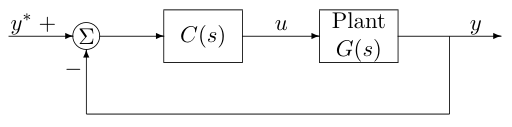
\includegraphics[width=1\linewidth]{figure/adaptive/robust.png} % width=...
    \caption{}
\end{subfigure}
  \begin{subfigure}{0.4\textwidth}
    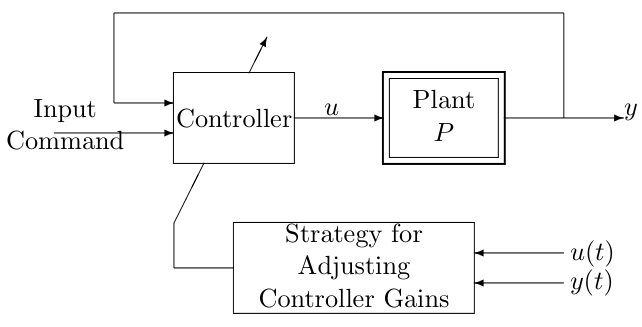
\includegraphics[width=1\linewidth]{figure/adaptive/adaptive_controller.png} % width=...
    \caption{}
\end{subfigure}
\caption{(a)鲁棒控制。(b)自适应控制。}
\label{adaptive_robust}
\end{figure}
  % \begin{description}
  %   \item[为什么采用自适应控制?]
    
  % \end{description}
鲁棒控制和自适应控制的对比如表 \ref{adaptive_robust_table}。
\newpage
  \begin{table}[htbp]
    \vspace{5pt}
    \caption{自适应控制与鲁棒控制的对比}
    \label{adaptive_robust_table}
    \setcellgapes{4pt}
    \makegapedcells
    \small
    \centering
    \begin{tabular}{p{0.46\textwidth}|p{0.46\textwidth}}
      \hline
      {\bf 自适应控制(adaptive control)} & {\bf 鲁棒控制(robust control)} \\
      \hline
      对于处理慢变或不变的参数不确定性上更有优势 & 在处理扰动、快变参数和未建模动态上更有优势\\
      \hline
      随着自适应过程的进行,自适应控制器能不断提高系统性能 & 鲁棒控制器试图使系统维持恒定的性能 \\
      \hline
      自适应控制器几乎不需要对于位置参数的先验({\it a priori})信息 & 鲁棒控制器需要对于参数的界有合理的先验估计\\
      \hline
    \end{tabular}
  \end{table}

\begin{description}
  \item[自适应控制的一般设计步骤] 
  \begin{enumerate}
    \item 描述/刻画闭环系统的期望特性;
    \item 设计合适的控制律,其中包含可调参数;
    \item 求出调节这些参数的自适应律;
    \item 分析待控制变量的收敛性,应用控制律。
  \end{enumerate}
\end{description}
\subsection{自适应控制的类型}
\begin{enumerate}
      \item 非直接型(间接型,indirect):估计被控对象(plant)参数 $\Rightarrow$ 设计控制器参数。首先确定过程(process)的模型与扰动特征,然后基于这些信息定出控制器参数。
      
      \item 直接型(direct):无需先确定过程(process)的模型与扰动特征,直接设计控制器参数。
\end{enumerate}
\begin{figure}[htbp]
  \centering
  \begin{subfigure}{0.45\textwidth}
    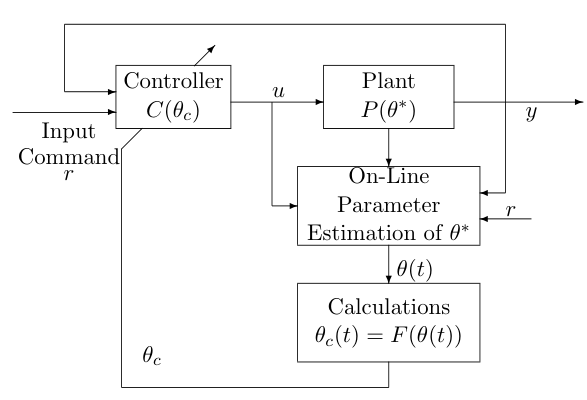
\includegraphics[width=1\linewidth]{figure/adaptive/indirect.png} % width=...
    \caption{}
\end{subfigure}
  \begin{subfigure}{0.45\textwidth}
    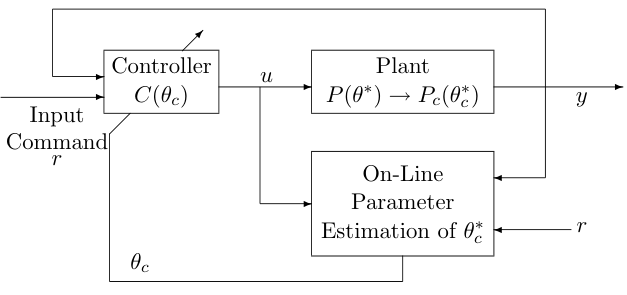
\includegraphics[width=1\linewidth]{figure/adaptive/direct.png} % width=...
    \caption{}
\end{subfigure}
\caption{(a)非直接型(间接型)。(b)直接型。}
\label{direct_indirect}
\end{figure}
\subsection{自适应控制的常用手段}
  \begin{description}
    \item[增益调节(Gain Scheduling)]
    \begin{enumerate}
      \item 事先建立一张表(lookup table),建立测量得的指标(或称为辅助量测值,auxiliary measurements,可理解为工作点)与参数的对应关系,
      控制器的增益就随着工作点而变化。
      
      \item 优点:当系统动力学改变时,参数可根据这些改变迅速变化。
      
      \item 缺点:参数的更新是开环的,并不会根据系统的演变而“学到”新的信息。
    \end{enumerate}
  \end{description}

  \begin{center}
  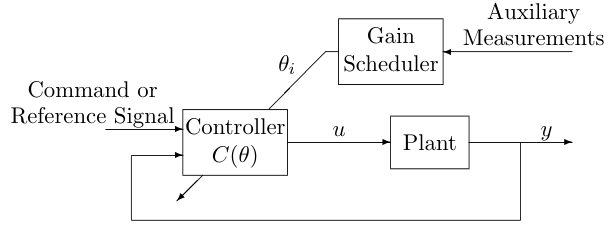
\includegraphics[scale=0.5]{figure/adaptive/gain_scheduling.png}
  \captionof{figure}{增益调节}
\end{center}
  \begin{description}
    \item[自调节控制器(Self-Tuning Controller,STC)]\index{自调节控制器(Self-Tuning Controller,STC)}
    \begin{enumerate}
      \item 控制器参数,是根据被控对象参数估计器所作出的参数估计实时计算的。
      
      \item 参数辨识和控制是同时进行的。
      
      \item 利用确定性等价原理(Certainty Equivalence Principle):将辨识所得的控制器参数当作真值,由此计算控制器参数。
    \end{enumerate}
  \end{description}
  \begin{center}
  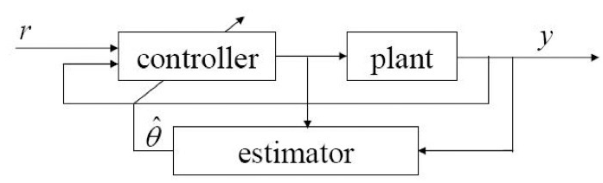
\includegraphics[scale=0.5]{figure/adaptive/stc.png}
  \captionof{figure}{自调节控制器}
\end{center}
  \begin{description}
    \item[模型参考自适应控制(Model Reference Adaptive Control, MRAC)]\index{模型参考自适应控制(Model Reference Adaptive Control, MRAC)}
    \begin{enumerate}
      \item 被控对象(plant):具有未知参数和确定的结构。
      
      \item 参考模型(reference model):指定系统目标输出。
      
      \item 反馈控制律:包含可调参数。
      
      \item 自适应机制:更新上述可调参数。
    \end{enumerate}
  \end{description}
\begin{figure}[htbp]
  \centering
  \begin{subfigure}{0.45\textwidth}
    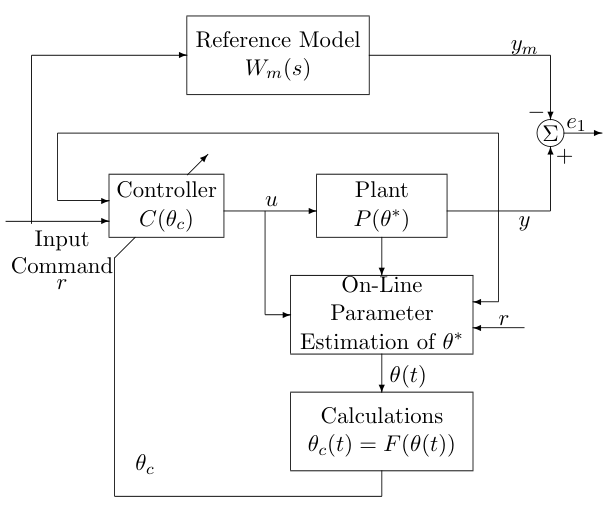
\includegraphics[width=1\linewidth]{figure/adaptive/indirect_MRAC.png} % width=...
    \caption{}
\end{subfigure}
  \begin{subfigure}{0.45\textwidth}
    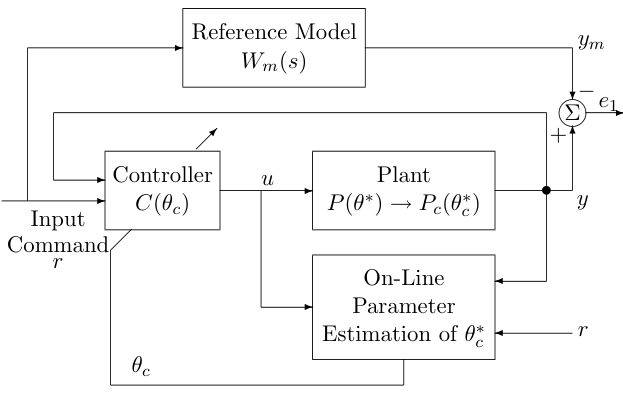
\includegraphics[width=1\linewidth]{figure/adaptive/direct_MRAC.png} % width=...
    \caption{}
\end{subfigure}
\caption{(a)非直接型(间接型)MRAC。(b)直接型MRAC。}
\end{figure}
\newpage
\section{标量系统的模型参考自适应控制}\label{4Bref}
\index{模型参考自适应控制(Model Reference Adaptive Control, MRAC)}
\subsection{引入}
考虑如下一阶标量系统
  \[ \dot{x} = a  x + u \]
  其中 $a$ 是{\bf 未知}参数,$x$ 为状态,$u$为控制输入。
  
  我们的控制目标是,设计$u$使得闭环系统中的所有信号都是有界的,且 $x$ 能够跟踪下述参考模型的参考状态  $x_{\ensuremath{\operatorname{ref}}}$:
  \[ \dot{x}_{\ensuremath{\operatorname{ref}}} = -
     a_{\ensuremath{\operatorname{ref}}} x_{\ensuremath{\operatorname{ref}}} +
     b_{\ensuremath{\operatorname{ref}}} u_c \]
  其中 $a_{\ensuremath{\operatorname{ref}}} > 0$ 且
  $b_{\ensuremath{\operatorname{ref}}}$ 已知,$u_c (t)$ 是(虚拟的)输入指令,其有界且分段连续。
  
  我们采用下述控制律
  \[ u^{\ast} = k^{\ast}_1 x + k^{\ast}_2 u_c \]
  那么
  \[\dot{x} = (a +  k^{\ast}_1) x + k^{\ast}_2 {u_c} \]
  如果能使得
  $a+  k^{\ast}_1=-a_{\ensuremath{\operatorname{ref}}},k^{\ast}_2=b_{\ensuremath{\operatorname{ref}}}$,
  即
  \begin{equation}\label{MRAC:intro}
      k^{\ast}_1 = - a - a_{\ensuremath{\operatorname{ref}}}, k^{\ast}_2 =  b_{\ensuremath{\operatorname{ref}}}
  \end{equation}
  那么\[\dot{x} = -a_{\ensuremath{\operatorname{ref}}} x + b_{\ensuremath{\operatorname{ref}}} {u_c} \]
  定义状态跟踪误差
  \[ e = x - x_{\ensuremath{\operatorname{ref}}} \]
  那么  
  \[ \dot{e} = \dot{x} - \dot{x}_{\ensuremath{\operatorname{ref}}} = -
  a_{\ensuremath{\operatorname{ref}}} e \]
  很明显随时间增长,$e\to 0$。也可通过作Lyapunov函数$V=e^2$来说明。这就实现了跟踪。
  但是$a$是未知的,因此 \eqref{MRAC:intro} 中的$k_1^\ast$无法直接应用。这时就有两种思路:
  \begin{itemize}
      \item 若采用直接型MRAC,我们直接估计控制器的参数,即直接估计$k_1^\ast$,将其记为$\hat{k}_1$,那么控制律就写成
      \[u=\hat{k}_1 x + b_{\ensuremath{\operatorname{ref}}} u_c\]
      \item 若采用间接型MRAC,我们则通过估计被控对象的参数转化得到控制器参数,即先估计$a$(记为$ \hat{a} (t)$),进而得到控制律
      \[u=(- \hat{a} (t) - a_{\ensuremath{\operatorname{ref}}}) x +
       b_{\ensuremath{\operatorname{ref}}} u_c\]
  \end{itemize}
\newpage
\subsection{标量系统的直接型MRAC设计}\label{sec:MRAC:scalar:direct}
考虑如下一阶系统
\begin{equation}
  \dot{x} = a  x + b  u \label{Sys:MRAC:scalar}
\end{equation}
其中 $a, b$为{\bf 未知}参数,$x$ 为状态,但$b$的符号$\sgn(b)$已知。

我们的控制目标是,设计$u$,使得闭环系统的所有信号都有界,且$x$能够跟踪下述参考模型的参考状态 $x_{\ensuremath{\operatorname{ref}}}$:
\begin{equation}
  \dot{x}_{\ensuremath{\operatorname{ref}}} = -
  a_{\ensuremath{\operatorname{ref}}} x_{\ensuremath{\operatorname{ref}}} +
  b_{\ensuremath{\operatorname{ref}}} u_c \label{Sys:MRAC:scalar:ref}
\end{equation}
其中 $a_{\ensuremath{\operatorname{ref}}} > 0$和
$b_{\ensuremath{\operatorname{ref}}}$为已知常数(是我们所期望的值),$u_c
(t)$是(虚拟的)输入指令,其有界且分段连续。

在不考虑模型参数未知的情况下,我们先采用以下控制律
\begin{equation}
  u = k^{\ast}_1 x + k^{\ast}_2 u_c \label{u*:k1*xk2*uc}
\end{equation}
其中 $k^{\ast}_1, k^{\ast}_2$ 是(我们所期望的)已知常数。这样,闭环系统 \eqref{Sys:MRAC:scalar} 就成为
\begin{align*}
  \dot{x} & = a  x + b  (k^{\ast}_1 x + k^{\ast}_2 u_c)\\
  & = (a + b  k^{\ast}_1)  x + b  k^{\ast}_2 u_c
\end{align*}
这样,对比 \eqref{Sys:MRAC:scalar:ref} 和上式就可得出,理想情况下跟踪参考模型时,参数
$k^{\ast}_1, k^{\ast}_2$应满足
\begin{equation}
  k^{\ast}_1 = \frac{-a - a_{\ensuremath{\operatorname{ref}}}}{b}, k^{\ast}_2 =
  \frac{b_{\ensuremath{\operatorname{ref}}}}{b} \label{k1*k2*}
\end{equation}

然而,当 $a, b$ 未知时,理想的 \eqref{k1*k2*} 无法实际应用。因此,将 \eqref{u*:k1*xk2*uc} 改造
为下述具有可调参数的控制律
\begin{equation}
  u = \hat{k}_1 (t) x + \hat{k}_2 (t) u_c \label{u:k1xk2uc}
\end{equation}
其中 $\hat{k}_1 (t), \hat{k}_2 (t)$ 分别是 $k^{\ast}_1,k^{\ast}_2$的{\bf 估计}。

将 \eqref{u:k1xk2uc} 代入 \eqref{Sys:MRAC:scalar} 有
\begin{equation}
  \dot{x} = (a + b \hat{k}_1 (t)) x + b \hat{k}_2 (t) u_c \label{Sys:MRAC:scalar:hat}
\end{equation}
定义{\bf 跟踪误差}
\begin{equation*}
  e \triangleq x - x_{\ensuremath{\operatorname{ref}}}
\end{equation*}
根据 \eqref{Sys:MRAC:scalar:ref} 和 \eqref{Sys:MRAC:scalar:hat},可推导出误差动力学是
\begin{align}
  \dot{e} & = \dot{x} - \dot{x}_{\ensuremath{\operatorname{ref}}}
  \nonumber\\
  & = (a + b \hat{k}_1 (t)) x + b \hat{k}_2 (t) u_c +
  a_{\ensuremath{\operatorname{ref}}} x_{\ensuremath{\operatorname{ref}}} -
  b_{\ensuremath{\operatorname{ref}}} u_c \nonumber\\
  & = (a + a_{\ensuremath{\operatorname{ref}}} + b \hat{k}_1 (t)) x + (b
  \hat{k}_2 (t) - b_{\ensuremath{\operatorname{ref}}}) u_c -
  a_{\ensuremath{\operatorname{ref}}} (x - x_{\ensuremath{\operatorname{ref}}}) \nonumber
\end{align}
结合 \eqref{k1*k2*},发现上式可写为
\[\dot{e} = - a_{\ensuremath{\operatorname{ref}}} e + b (\hat{k}_1(t)-k^{\ast}_1) x + b (\hat{k}_2 (t) - k^{\ast}_2) u_c\]
第二项和第三项中的括号可理解为对$k^{\ast}_1,k^{\ast}_2$的参数估计误差,于是定义
\[\tilde{k}_1 \triangleq\hat{k}_1 (t) - k^{\ast}_1,\tilde{k}_2 \triangleq \hat{k}_2
(t) - k^{\ast}_2\]则有
\begin{equation}
  \dot{e} = - a_{\ensuremath{\operatorname{ref}}} e + b \tilde{k}_1 x + b 
  \tilde{k}_2 u_c  \label{err:MRAC:scalar}
\end{equation}

下面的目标是让各误差$e,\tilde{k}_1,\tilde{k}_2$收敛至$0$,进而使$x$跟踪$x_\mathrm{ref}$。
考虑候选Lyapunov函数
\begin{equation}
  V = \frac{1}{2} e^2 + \frac{1}{2} \tilde{k}^2_1 + \frac{1}{2} \tilde{k}^2_2\label{not_implement_candidate}
\end{equation}
沿 \eqref{err:MRAC:scalar} 的状态轨线,求其对时间的导数得(注意$\dot{\tilde{k}}_1=\dot{\hat{k}}_1$,$\dot{\tilde{k}}_2=\dot{\hat{k}}_2$)
\begin{align}
  \dot{V} & = e  \dot{e} + \tilde{k} _1 \dot{\hat{k}}_1 + \tilde{k} _2
  \dot{\hat{k}}_2 \nonumber\\
  & = - a_{\ensuremath{\operatorname{ref}}} e^2 + b \tilde{k} _1 x  e + b
  \tilde{k} _2 u_c e + \tilde{k} _1 \dot{\hat{k}}_1 + \tilde{k} _2
  \dot{\hat{k}}_2 \label{not_implement_vdot_mid}\\
  & = - a_{\ensuremath{\operatorname{ref}}} e^2 + \tilde{k} _1
  (\dot{\hat{k}}_1 + b  x  e) + \tilde{k} _2 (\dot{\hat{k}}_2 + b  u_c e) \label{not_implement_vdot}
\end{align}
如果我们将第二项与第三项消去,即选取
\begin{equation*}
  \dot{\hat{k}}_1 = - b  x  e, \dot{\hat{k}}_2 = - b  u_c e
  % \label{k1k2:not:implemented}
\end{equation*}
则可得 $\dot{V} \leq 0$。然而,由于 $b$ 未知,上式不能直接应用。
% \eqref{k1k2:not:implemented}。

我们发现,如果在 \eqref{not_implement_candidate} 的第二、三项中乘上$b$,那么 \eqref{not_implement_vdot} 的后两项中
$b$就可提出,进而设计$\dot{\hat{k}}_1,\dot{\hat{k}}_2$消去的项就不含有$b$。然而,由于$b$可能为负,所以可能使$V$不再正定。
于是,考虑加入$|b|$,这样虽会产生$\sgn(b)$,但其已知。进而,考虑下述候选Lyapunov函数:
\begin{equation}
  V = \frac{1}{2} e^2 + \frac{| b |}{2 \gamma_1} \tilde{k}^2_1 + \frac{| b
  |}{2 \gamma_2} \tilde{k}^2_2 \label{Lyafun:ek1k2}
\end{equation}
其中 $\gamma_1, \gamma_2 > 0$。
沿 \eqref{err:MRAC:scalar} 的状态轨线,求其对时间的导数得(在 \eqref{not_implement_vdot_mid} 的基础上改写,注意$\sgn(b)|b|=\sgn^2(b)b=b$)
\begin{align*}
    \dot{V}   &= - a_{\ensuremath{\operatorname{ref}}} e^2 + \frac{ | b |}{\gamma_1} \sgn(b) \gamma_1 \tilde{k} _1 x  e + \frac{| b |}\sgn(b){\gamma_2} \gamma_2
  \tilde{k} _2 u_c e + \frac{| b |}{\gamma_1}\tilde{k} _1 \dot{\hat{k}}_1 + \frac{| b |}{\gamma_2}\tilde{k} _2
  \dot{\hat{k}}_2 \\
    & = - a_{\ensuremath{\operatorname{ref}}} e^2 + \frac{| b
   |}{\gamma_1} \widetilde{ k} _1 (\dot{\hat{k}}_1 + \gamma_1
   \ensuremath{\operatorname{sgn}} (b) x  e) + \frac{| b |}{\gamma_2}
   \tilde{k} _2 (\dot{\hat{k}}_2 + \gamma_2 \ensuremath{\operatorname{sgn}}
   (b)  u_c e)
\end{align*}
此时,如果我们选取
\begin{equation*}
  \dot{\hat{k}}_1 = -  \gamma_1 \ensuremath{\operatorname{sgn}} (b) x  e,
  \dot{\hat{k}}_2 = -  \gamma_2 \ensuremath{\operatorname{sgn}} (b)  u_c e
\end{equation*}
则
\begin{equation*}
  \dot{V} = - a_{\ensuremath{\operatorname{ref}}} e^2 \leq 0
\end{equation*}
从而$V (t) \leq V (0)$。由 \eqref{Lyafun:ek1k2} 的形式得$e, \tilde{k} _1,
\tilde{k} _2$ 都有界,于是$u$有界;又由于$x_\mathrm{ref}$和$u_c$有界,因此 $x$有界。

再求一次导得$\ddot{V} = - 2a_{\ensuremath{\operatorname{ref}}} e  \dot{e}$,将误差动力学 \eqref{err:MRAC:scalar} 代入,发现其也有界。

因此根据 Barbalat引理(\ref{barbalat}),$\lim\limits_{t \rightarrow \infty}
\dot{V} (t) = 0$,也即 $\lim\limits_{t \rightarrow \infty} e (t) = 0$。

\begin{table}[htbp]
  \centering
  \setcellgapes{4pt}
  \makegapedcells
  \caption{标量系统的直接型MRAC设计汇总}
  \begin{tabular}{p{4.0cm}p{10.0cm}}
    \hline
    开环被控对象 & $\dot{x} = - a  x + b  u$; $\{ a, b \}$ 未知,但
    $\ensuremath{\operatorname{sgn}} (b)$ 已知\\
    参考模型 & $\dot{x}_{\ensuremath{\operatorname{ref}}} = -
    a_{\ensuremath{\operatorname{ref}}} x_{\ensuremath{\operatorname{ref}}} +
    b_{\ensuremath{\operatorname{ref}}} u_c$\\
    跟踪误差 & $e \triangleq x - x_{\ensuremath{\operatorname{ref}}}$\\
    控制输入 & $u = \hat{k}_1 (t) x + \hat{k}_2 (t) u_c$\\
    直接型MRAC控制律& $\dot{\hat{k}}_1 = -  \gamma_1
    \ensuremath{\operatorname{sgn}} (b) x  e, \dot{\hat{k}}_2 = -  \gamma_2
    \ensuremath{\operatorname{sgn}} (b)  u_c e ; \gamma_1, \gamma_2 > 0$\\
    \hline
  \end{tabular}
\end{table}

总结设计步骤:
\begin{enumerate}
  \item 根据已知参数,寻求一种控制器结构
  
  \item 导出误差动力学(包括跟踪误差和参数估计误差)
  
  \item 根据上述误差构造 Lyapunov函数
  
  \item 设计参数更新规则,使得 $\dot{V} \leq 0$
\end{enumerate}
\subsection{具有非线性项的标量系统的直接型MRAC设计}

考虑如下标量系统
\begin{equation}
  \dot{x} = a  x + b  (u + f (x)) \label{Sys:MRAC:nonlinear}
\end{equation}
其中 $f (x) = \varphi (x) \theta$, $\varphi$ 有界、连续且已知; $a, b, \theta$ 是未知的参数,$b$的符号$\sgn(b)$已知。

仍定义参考模型如式 \eqref{Sys:MRAC:scalar:ref}。
我们试图消去$f$,于是在  \eqref{u:k1xk2uc} 基础上提出下述控制律:
\begin{equation*}
  u = \hat{k}_1 (t) x + \hat{k}_2 (t) u_c - \varphi (x) \theta
\end{equation*}
但是$\theta$是未知的,所以将它换成它的估计$\hat{\theta} (t)$,得到
\begin{equation}
  u = \hat{k}_1 (t) x + \hat{k}_2 (t) u_c - \varphi (x) \hat{\theta} (t)
\end{equation}
代入 \eqref{Sys:MRAC:nonlinear} 得到闭环系统方程
\begin{equation}
    \dot{x} = a  x +  b \hat{k}_1 (t) x + b \hat{k}_2 (t) u_c - b \varphi
   (x) (\hat{\theta} (t) - \theta) \label{Closed_form_scalar_nonlinear}
\end{equation}
类似上一小节对于理想情形的推导,可得与 \eqref{k1*k2*} 一样的$k^{\ast}_1, k^{\ast}_2$。仍定义$e=x-x_{\operatorname{ref}}$,结合 \eqref{Sys:MRAC:scalar:ref} 与 \eqref{Closed_form_scalar_nonlinear},误差动力学可写为
\begin{align}
  \dot{e} & =  a  x +  b \hat{k}_1 (t) x + b \hat{k}_2 (t) u_c - b \varphi
  (x) (\hat{\theta} (t) - \theta) + a_{\ensuremath{\operatorname{ref}}}
  x_{\ensuremath{\operatorname{ref}}} - b_{\ensuremath{\operatorname{ref}}}
  u_c \nonumber\\
  & = (a_{\ensuremath{\operatorname{ref}}} + a) x +  b \hat{k}_1 (t) x +
  (b \hat{k}_2 (t) - b_{\ensuremath{\operatorname{ref}}}) u_c - b \varphi (x)
  (\hat{\theta} (t) - \theta) - a_{\ensuremath{\operatorname{ref}}} (x-x_{\operatorname{ref}})
  \nonumber\\
  & =  b (\hat{k}_1 (t) - k^{\ast}_1) x + b (\hat{k}_2 (t) - k^{\ast}_2)
  u_c - b \varphi (x) (\hat{\theta} (t) - \theta) -
  a_{\ensuremath{\operatorname{ref}}} e \nonumber\\
  & =  - a_{\ensuremath{\operatorname{ref}}} e + b \tilde{k}_1 x + b
  \tilde{k}_2 u_c - b \varphi \tilde{\theta}  \label{err:MRAC:nonlinear}
\end{align}
其中定义了三个参数估计误差 $\tilde{k}_1 \triangleq \hat{k}_1 (t) - k^{\ast}_1$, $\tilde{k}_2 \triangleq \hat{k}_2
(t) - k^{\ast}_2$ 和 $\tilde{\theta} \triangleq\hat{\theta} (t) - \theta$。

类似上一小节(使括号中的$b$可提出)的思路,考察下述候选Lyapunov函数
\begin{equation}
  V = \frac{1}{2} e^2 + \frac{| b |}{2 \gamma_1} \tilde{k}^2_1 + \frac{| b
  |}{2 \gamma_2} \tilde{k}^2_2 + \frac{| b |}{2 \gamma_3} \tilde{\theta}^2 
  \label{Lyafun:ek1k2j}
\end{equation}
其中 $\gamma_1, \gamma_2, \gamma_3 > 0$.

沿 \eqref{err:MRAC:nonlinear} 的状态轨线,求其对时间的导数得
\begin{align*}
  \dot{V} & =  e  \dot{e} + \frac{| b |}{\gamma_1} \widetilde{ k} _1
  \dot{\hat{k}} _1 + \frac{| b |}{\gamma_2} \tilde{k} _2 \dot{\hat{k}} _2 +
  \frac{| b |}{\gamma_3} \tilde{\theta}  \dot{\hat{\theta}}\\
  & =  - a_{\ensuremath{\operatorname{ref}}} e^2 + \frac{| b |}{\gamma_1}
  \widetilde{ k} _1 (\dot{\hat{k}}_1 + \gamma_1
  \ensuremath{\operatorname{sgn}} (b) x  e) + \frac{| b |}{\gamma_2} \tilde{k}
  _2 (\dot{\hat{k}}_2 + \gamma_2 \ensuremath{\operatorname{sgn}} (b)  u_c e) +
  \frac{| b |}{\gamma_3} \tilde{\theta} (\dot{\hat{\theta}} - \gamma_3
  \ensuremath{\operatorname{sgn}} (b)   \varphi e)
\end{align*}
我们选取
\begin{equation*}
  \dot{\hat{k}}_1 = -  \gamma_1 \ensuremath{\operatorname{sgn}} (b) x  e,
  \dot{\hat{k}}_2 = -  \gamma_2 \ensuremath{\operatorname{sgn}} (b)  u_c e,
  \dot{\hat{\theta}} = \gamma_3 \ensuremath{\operatorname{sgn}} (b)   \varphi e
\end{equation*}
即得
\begin{equation*}
  \dot{V} = - a_{\ensuremath{\operatorname{ref}}} e^2 \leq 0
\end{equation*}
因此$V (t) \leq V (0)$。由 \eqref{Lyafun:ek1k2j} 的形式得$e, \tilde{k} _1,
\tilde{k} _2, \tilde{\theta}$ 都有界,于是$u$有界;又由于$x_\mathrm{ref}$和$u_c$有界,因此 $x$有界。

再求一次导有$ \ddot{V} = - 2 a_{\ensuremath{\operatorname{ref}}} e  \dot{e} $,将误差动力学 \eqref{err:MRAC:nonlinear} 代入,$\ddot{V}$ 有界。

因此根据 Barbalat引理(\ref{barbalat}), $\lim\limits_{t \rightarrow \infty}
\dot{V} (t) = 0$,也即 $\lim\limits_{t \rightarrow \infty} e (t) = 0$。

\begin{problem}
将 \eqref{Sys:MRAC:nonlinear} 改为
  \[ \dot{x} = a  x + b  u + \varphi(x) \theta \]
如何设计自适应控制律?
\end{problem}
\begin{hint}
考虑如下自适应律
\[ u = \hat{k}_1 (t) x + \hat{k}_2 (t) u_c - \varphi (x)
       \frac{\hat{\theta} (t)}{\hat{b} (t)} \triangleq \hat{k}_1 (t) x +
       \hat{k}_2 (t) u_c - \varphi (x) \hat{\theta}_1 (t) \]
\end{hint}


\subsection{标量系统的非直接型MRAC设计}

考虑如下一阶标量系统
\begin{equation}
  \dot{x} = a x + b  u \label{Sys:Indirect:MRAC:scalar}
\end{equation}
其中 $a, b$ 为未知参数。

参考状态和参考模型定义如式 \eqref{Sys:MRAC:scalar:ref}。
类似上面两节,理想情况下应有
\begin{equation}
  k^{\ast}_1 = \frac{-a - a_{\ensuremath{\operatorname{ref}}}}{b}, k^{\ast}_2 =
  \frac{b_{\ensuremath{\operatorname{ref}}}}{b}
  \label{Sys:Indirect:MRAC:scalar:perfect}
\end{equation}
采用下述控制律
\begin{equation}
  u = \hat{k}_1 (t) x + \hat{k}_2 (t) u_c\label{Law:Indirect:MRAC:scalar}
\end{equation}
在 \ref{sec:MRAC:scalar:direct} 小节所述的设计过程中,我们设计的自适应律直接更新$\hat{k}_1 (t), \hat{k}_2 (t)$。而在本小节的设计中,我们利用
\eqref{Sys:Indirect:MRAC:scalar:perfect} 陈述的理想对应关系,并将其中的未知参数$a$和$b$换成其估计,进而得到 $\hat{k}_1 (t), \hat{k}_2 (t)$ 如下
\[ \hat{k}_1 (t) = \frac{\hat{a} -
   a_{\ensuremath{\operatorname{ref}}}}{\hat{b}}, \hat{k}_2 (t) =
   \frac{b_{\ensuremath{\operatorname{ref}}}}{\hat{b}} \]
将其代入 \eqref{Law:Indirect:MRAC:scalar},即得
\begin{equation}
  u = \frac{1}{\hat{b}} [-(\hat{a} + a_{\ensuremath{\operatorname{ref}}}) x +
  b_{\ensuremath{\operatorname{ref}}} u_c] \label{u:before:modification}
\end{equation}
将 \eqref{u:before:modification} 代入 \eqref{Sys:Indirect:MRAC:scalar} 有
\begin{align}
  \dot{x} & = (a - \hat{a} + \hat{a})  x + (b - \hat{b} + \hat{b} ) u
  \nonumber\\
  & = -(\hat{a} - a)  x -(\hat{b} -b)  u + \hat{a} x + \hat{b} u \nonumber\\
  & = -(\hat{a} - a)  x -(\hat{b} -b)  u + \hat{a} x + [-(\hat{a} + a_{\ensuremath{\operatorname{ref}}}) x +
  b_{\ensuremath{\operatorname{ref}}} u_c]\nonumber \\
  & = -(\hat{a} - a)  x -(\hat{b} -b)  u -a_{\ensuremath{\operatorname{ref}}} x +
  b_{\ensuremath{\operatorname{ref}}} u_c \nonumber
\end{align}
令参数估计误差 $\tilde{a}  \triangleq \hat{a} - a$ and $\tilde{b}  \triangleq \hat{b} -b$,则上式写为
\begin{equation*}
   \dot{x}  = -\tilde{a}  x - \tilde{b}  u - a_{\ensuremath{\operatorname{ref}}} x +
  b_{\ensuremath{\operatorname{ref}}} u_c
\end{equation*}
仍定义$e=x-x_{\operatorname{ref}}$,于是误差动力学可写为
\begin{equation}
  \dot{e} =\dot{x}-\dot{x}_{\operatorname{ref}}= - a_{\ensuremath{\operatorname{ref}}} (x-x_{\operatorname{ref}})- \tilde{a}  x - \tilde{b}u= -a_{\ensuremath{\operatorname{ref}}} e - \tilde{a}  x - \tilde{b}u\label{error_dyn_indirect}
\end{equation}

下面的目标是让各误差$e,\tilde{a},\tilde{b}$收敛至$0$,进而使$x$跟踪$x_\mathrm{ref}$。考虑下述候选 Lyapunov 函数
\begin{equation*}
  V = \frac{1}{2} e^2 + \frac{1}{2 \gamma_1} \tilde{a}^2  + \frac{1}{2
  \gamma_2} \tilde{b}^2 
\end{equation*}
其中$\gamma_1,\gamma_2>0$。沿 \eqref{error_dyn_indirect},求$V$对时间的导数得
\begin{align*}
  \dot{V} & = - a_{\ensuremath{\operatorname{ref}}} e^2 + \frac{1}{\gamma_1}
  \tilde{a} (\dot{\hat{a}} - \gamma_1 e  x) + \frac{1}{\gamma_2} \tilde{b}
  (\dot{\hat{b}} - \gamma_2  e  u)
\end{align*}
如果选取
\begin{equation}
  \dot{\hat{a}}  = \gamma_1 e  x, \dot{\hat{b}}  = \gamma_2 e  u
  \label{a-bar-b-bar:before:modification}
\end{equation}
我们可得 \[\dot{V} = - a_{\ensuremath{\operatorname{ref}}} e^2 \leq 0\]

根据$V$的形式得$e, \tilde{a}, \tilde{b} \in \mathbf{L}_{\infty}$。由于
$x_{\ensuremath{\operatorname{ref}}} \in \mathbf{L}_{\infty}$ 且 $a, b$ 为常数,我们可得$x, \hat{a}, \hat{b} \in \mathbf{L}_{\infty}$。对$V$再求一次导得
$ \ddot{V} = - 2 a_{\ensuremath{\operatorname{ref}}} e  \dot{e} $,则只要说明$\dot{e}$的有界性,即可用Barbalat引理。这其中只有$u$的有界性还无法保证。
我们注意到,此时的$u$的形式不同于之前——在分母上出现了$\hat{b}$。
为了说明$u$的有界性(这也保证自适应律能够物理实现),我们需要对自适应律作出适当修改,避免 $\hat{b} (t)$ 越过$0$。通过一些先验知识,这样的修改是可以完成的。

{\bf 先验假设}:$\ensuremath{\operatorname{sgn}} (b)$ 和 $| b |$的容许下界
$b_{\min} > 0$ 已知。

据此,我们将 \eqref{a-bar-b-bar:before:modification} 的第二式修改为
\begin{equation}\dot{\hat{b}}(t)=\begin{cases}
  \gamma_2ue&\text{若}\ |\hat{b}|>b_{\min}\ \text{或}\ |\hat{b}|=b_{\min}\ \text{且}\ ue\sgn(b)\ge 0\\
  0&\text{其他}
\end{cases}\label{b:bar:modification}
\end{equation}
作出这种修正的动机,就是使$\hat{b}$在其(绝对值)太小,且还欲继续减小时停止变化。

我们需要说明,形如 \eqref{b:bar:modification}  的修正在确保$\hat{b}$不越过允许边界的同时,还能保证系统稳定。按照 \eqref{a-bar-b-bar:before:modification} 第一式,$\dot{V}$的第二项已消去,第一项已为半负定,则说明最后一项
\begin{equation}
    \tilde{b} (\dot{\hat{b}} - \gamma_2 e  u) \leq 0 \label{last_term}
\end{equation}
即可。

我们只需检验 $| \hat{b} | = b_{\min}
$且$u  e  \ensuremath{\operatorname{sgn}} (b) < 0$的情况(另一种情况,上式一定为$0$)。此时
$\dot{\hat{b}} = 0$,于是上式左侧等于$ - \tilde{b} e  u = - (\hat{b} - b)
\ensuremath{\operatorname{sgn}} (b) \cdot u  e 
\ensuremath{\operatorname{sgn}} (b)$。
下面分情况讨论:
\begin{itemize}[leftmargin=1em]
    \item 若$\ensuremath{\operatorname{sgn}} (b) > 0$,则$ue<0$, $\hat{b} = b_{\min}\leq b$,因此$\hat{b} - b \leq 0$,故$- \tilde{b} e  u\le 0$;
    \item 若$\ensuremath{\operatorname{sgn}} (b) < 0$,则$ue>0$, $\hat{b} = -b_{\min}\geq b$,因此$\hat{b} - b \geq 0$,故$- \tilde{b} e  u\le 0$。
\end{itemize}
于是,在修正 \eqref{b:bar:modification} 下,\eqref{last_term} 成立。
则
\begin{equation*}
  \dot{V} \leq - a_{\ensuremath{\operatorname{ref}}} e^2 \leq 0
  \label{V:under:modification}
\end{equation*}
同前可得$e,\tilde{a},\tilde{b},x, \hat{a}, \hat{b} \in \mathbf{L}_{\infty}$;根据修正可得$ u, \dot{e}\in \mathbf{L}_{\infty}$。但此时不能简单利用Barbalat引理——因为$\ddot{V}$的形式变了。解决方法是,对 \eqref{V:under:modification} 两边积分,有
\[ V (t) - V (0) \leq -a_{\ensuremath{\operatorname{ref}}} \int^t_0 e^2 (\tau)   \diff  \tau \leq 0 \]
\[ \Rightarrow \int^t_0 e^2 (\tau) \diff  \tau \leq
   \frac{1}{a_{\ensuremath{\operatorname{ref}}}} (V (0) - V (t)) \leq
   \frac{1}{a_{\ensuremath{\operatorname{ref}}}} V (0) \]
则$e (t) \in \mathbf{L}_2$。根据推论 \ref{barbalat_cor_1},则
$ \lim\limits_{t \rightarrow  \infty} e (t) = 0$。

\begin{table}[htbp]
  \centering
  \setcellgapes{4pt}
  \makegapedcells
  \caption{标量系统的非直接型MRAC设计汇总}
  \begin{tabular}{p{4.0cm}p{10.0cm}}
  \hline
   开环被控对象 & $\dot{x} =  a  x + b  u$\\
    参考模型 & $\dot{x}_{\ensuremath{\operatorname{ref}}} = -
    a_{\ensuremath{\operatorname{ref}}} x +
    b_{\ensuremath{\operatorname{ref}}} u_c, a_{\operatorname{ref}}>0$\\
    跟踪误差 & $e = x - x_{\ensuremath{\operatorname{ref}}}$\\
    控制输入 & $u = \frac{1}{\hat{b}} [(\hat{a} -
    a_{\ensuremath{\operatorname{ref}}}) x +
    b_{\ensuremath{\operatorname{ref}}} u_c]$\\
    非直接型 MRAC 控制律 & {\hspace{7em}}$\dot{\hat{a}}  =  \gamma_1 e  x$
    
    $\dot{\hat{b}}(t)=\begin{cases}
  \gamma_2ue&\text{若}\ |\hat{b}|>b_{\min}\ \text{或}\ |\hat{b}|=b_{\min}\ \text{且}\ ue\sgn(b)\ge 0\\
  0&\text{其他}
\end{cases}$\\
    \hline
  \end{tabular}
\end{table}



\section{多输入多输出(MIMO)系统的模型参考自适应控制}\label{4Cref}
考虑下述线性系统
\begin{equation}
  \dot{x} = A  x + B \Lambda u\label{Sys:MRAC:MIMO}
\end{equation}
其中 $x \in \mathbf{R}^n$是系统的状态, $u \in \mathbf{R}^m$ 是控制输入,$B \in \mathbf{R}^{n \times m}$ 是已知的控制矩阵,而 $A \in \mathbf{R}^{n \times n}, \Lambda \in \mathbf{R}^{m \times m}$ 是未知的常值矩阵。又假设  $\Lambda$ 是对角阵,且对角线上均为正数,且$(A, B \Lambda)$ 可控。$\Lambda$是不确定的,这是用于刻画控制失效或建模不准确,意即控制增益可能不确定,或是设计者估计的系统控制效果可能是不准确的。

{\bf 控制目标是:}设计$u$,使得闭环系统的所有信号都有界,且$x$能够跟踪下述参考模型的参考状态 $x_{\ensuremath{\operatorname{ref}}}$:
 \begin{equation}
    \dot{x}_{\ensuremath{\operatorname{ref}}} =
    A_{\ensuremath{\operatorname{ref}}} x_{\ensuremath{\operatorname{ref}}} +
    B_{\ensuremath{\operatorname{ref}}} u_c\label{ideal_mimo}
  \end{equation}
其中$A_{\ensuremath{\operatorname{ref}}} \in \mathbf{R}^{n \times n}$ 是Hurwitz的,$B_{\ensuremath{\operatorname{ref}}} \in \mathbf{R}^{n \times m}$, $u_c \in \mathbf{R}^m$ 是有界的(虚拟)输入指令。

首先推导理想情形。若$A \in \mathbf{R}^{n \times n}$ 与 $\Lambda \in \mathbf{R}^{m\times m}$ 已知,我们可选用如下控制律
\[ u = K^{\ast}_1 x + K^{\ast}_2 u_c \]
其中 $K^{\ast}_1 \in \mathbf{R}^{m \times n}, K^{\ast}_2 \in \mathbf{R}^{m
\times m}$,将上式代入 \eqref{Sys:MRAC:MIMO} 可得
\[ \dot{x} = (A + B \Lambda K^{\ast}_1) x + B \Lambda K^{\ast}_2 u_c \]
与理想情形对比可知
\begin{equation}
  \left\{\begin{array}{l}
    A + B \Lambda K^{\ast}_1 = A_{\ensuremath{\operatorname{ref}}}\\
    B \Lambda K^{\ast}_2 = B_{\ensuremath{\operatorname{ref}}}
  \end{array}\right. \label{matching:condition:GLS}
\end{equation}
上式称为匹配条件(matching conditions)。我们应注意,一般地,无法保证满足 \eqref{matching:condition:GLS} 的理想增益阵$K^{\ast}_1, K^{\ast}_2$存在。不过,在实际应用中,如果$A, B$的结构已知,可以设计 $A_{\ensuremath{\operatorname{ref}}}, B_{\ensuremath{\operatorname{ref}}}$ 以保证 \eqref{matching:condition:GLS} 有解。

下面假设满足 \eqref{matching:condition:GLS} 的$K^{\ast}_1, K^{\ast}_2$存在(there is sufficient structure flexibility to meet the control
objective)。由于$\Lambda$未知,我们提出以下含可变矩阵参数的控制律
\[ u = \hat{K}_1 (t) x + \hat{K}_2 (t) u_c \]
代入 \eqref{Sys:MRAC:MIMO} 可得
\begin{align}
    \dot{x}&=A  x + B \Lambda (\hat{K}_1 (t) x + \hat{K}_2 (t) u_c)+
    \underbrace{A_{\ensuremath{\operatorname{ref}}} x +
    B_{\ensuremath{\operatorname{ref}}} u_c-A_{\ensuremath{\operatorname{ref}}} x -
    B_{\ensuremath{\operatorname{ref}}} u_c}_{\text{增减期望形式}}\nonumber\\
    &=A_{\ensuremath{\operatorname{ref}}} x +
    B_{\ensuremath{\operatorname{ref}}} u_c+(A + B \Lambda \hat{K}_1 (t)-A_{\ensuremath{\operatorname{ref}}}) x+(B\Lambda\hat{K}_2 (t)-B_{\ensuremath{\operatorname{ref}}}) u_c\nonumber\\
    &=A_{\ensuremath{\operatorname{ref}}} x +
    B_{\ensuremath{\operatorname{ref}}} u_c+(B \Lambda \hat{K}_1 (t)-B \Lambda K^{\ast}_1) x+(B\Lambda\hat{K}_2 (t)-B \Lambda K^{\ast}_2) u_c\label{mimo_dotx}
\end{align}
第三行是将 \eqref{matching:condition:GLS} 代入。记参数估计误差 $\tilde{K}_1 \triangleq \hat{K}_1 {- K_1^{\ast}} , \tilde{K}_2
\triangleq \hat{K}_2 {- K_2^{\ast}} $,则
\[ \dot{x} = A_{\ensuremath{\operatorname{ref}}}  x +
   B_{\ensuremath{\operatorname{ref}}} u_c + B \Lambda  \tilde{K}_1 x + B
   \Lambda  \tilde{K}_2 u_c \]

定义跟踪误差 $e \triangleq x -
x_{\ensuremath{\operatorname{ref}}}$。根据 \eqref{ideal_mimo} 和 \eqref{mimo_dotx},写出误差动力学
\begin{equation}
  \dot{e} = A_{\ensuremath{\operatorname{ref}}} e + B \Lambda  \tilde{K}_1 x +
  B \Lambda  \tilde{K}_2 u_c \label{errsys:MRAC:GLS}
\end{equation}
类比之前的构造,考虑如下“形式上的”Lyapunov函数
\begin{align*}
  V&=\frac12e^2+\frac{1}{2}\tilde{K}_1^2+\frac{1}{2}\tilde{K}_2^2
\end{align*}
由于其中的$e,\tilde{K}_1,\tilde{K}_2$都是向量或矩阵,而Lyapunov函数输出是标量,上式要做相应的修改。

首先,将$\frac12e^2$换成$\frac12e^\mathrm{T}e$。求其导数得\[e^\mathrm{T}\dot{e}=e^\mathrm{T}A_{\ensuremath{\operatorname{ref}}} e+\dots\]
省略的项待与后面的项合并。仅考察第一项,我们发现由于$A_{\ensuremath{\operatorname{ref}}}$未必负定,则第一项并不保证为负定。后续若要类似之前思路保留该项则不可行。考虑重新设计此项为\[e^\mathrm{T}\textcolor{second}{P}e\]
其中$P$为正定阵。则此项导数是
\[e^\mathrm{T}P\dot{e}+\dot{e}^\mathrm{T}Pe=e^\mathrm{T}(A_{\ensuremath{\operatorname{ref}}}^\mathrm{T} P + P A_{\ensuremath{\operatorname{ref}}}) e+\dots\]
由于 $A_{\ensuremath{\operatorname{ref}}}$ 是 Hurwitz的,根据定理 \ref{linearlya},我们可知对任意正定矩阵 $Q \in \mathbf{R}^{n \times
n}$,都存在唯一正定阵 $P \in \mathbf{R}^{n \times n}$
使得
\[ A_{\ensuremath{\operatorname{ref}}}^\mathrm{T} P + P 
   A_{\ensuremath{\operatorname{ref}}} = - Q < 0 \]
则第一项必为负定。

然后,将$\tilde{K}_1^2$换为\[\tr(\tilde{K}_1^\mathrm{T}\tilde{K}_1)\]
由 \ref{pd_npd_div},$\tilde{K}_1^\mathrm{T}\tilde{K}_1$ 是半正定的,进而由 \ref{pd_nd_thm},其特征值全为非负,则其迹一定非负,则上式是半正定的。

下面说明$\tr(\tilde{K}_1^\mathrm{T}\tilde{K}_1)=0\iff \tilde{K}_1=0$。仅证“$\implies$”情形。由于$\tilde{K}_1^\mathrm{T}\tilde{K}_1$特征值非负,所以迹为$0$就表明所有特征值均为$0$。则由 \ref{ortho_sim_diag},存在正交矩阵$S$使得$S^{-1}\tilde{K}_1^\mathrm{T}\tilde{K}_1S=0$。则$\tilde{K}_1^\mathrm{T}\tilde{K}_1=0$。因此对于所有$x\in\mathbf{R}^{n}$均有$x^{\mathrm{T}}\tilde{K}_1^\mathrm{T}\tilde{K}_1x=0$,因此$\tilde{K}_1x=0$,则$\tilde{K}_1=0$。因此,$\tr(\tilde{K}_1^\mathrm{T}\tilde{K}_1)$正定。

类似将$\tilde{K}_2^2$换为$\tr(\tilde{K}_2^\mathrm{T}\tilde{K}_2)$。
于是考虑如下候选Lyapunov函数
\begin{equation}\label{MODMIMOLYA:modify1}
V=e^\mathrm{T}Pe+\tr(\tilde{K}_1^\mathrm{T}\tilde{K}_1)+\tr(\tilde{K}_2^\mathrm{T}\tilde{K}_2)
\end{equation}

求其导数得(注意$\dot{\tilde{K}}_1=\dot{\hat{K}}_1$,$\dot{\tilde{K}}_2=\dot{\hat{K}}_2$)
\begin{align*}
  \dot{V} & =e^\mathrm{T}P\dot{e}+\dot{e}^\mathrm{T}Pe + 2\ensuremath{\operatorname{tr}} \{
  \tilde{K}^\mathrm{T}_1 \dot{\hat{K}} _1 \} + 2\ensuremath{\operatorname{tr}}
  \{ \tilde{K}^\mathrm{T}_2 \dot{\hat{K}} _2 \}\\
  & = e^\mathrm{T}P( A_{\ensuremath{\operatorname{ref}}} e + B \Lambda  \tilde{K}_1 x +
  B \Lambda  \tilde{K}_2 u_c)+(A_{\ensuremath{\operatorname{ref}}} e + B \Lambda  \tilde{K}_1 x +
  B \Lambda  \tilde{K}_2 u_c)^\mathrm{T}Pe\\
  &\quad+
  2\ensuremath{\operatorname{tr}} \{ \tilde{K}^\mathrm{T}_1 \dot{\hat{K}} _1 \}
  + 2\ensuremath{\operatorname{tr}} \{ \tilde{K}^\mathrm{T}_2 \dot{\hat{K}} _2 \}\\
  & = e^\mathrm{T}(A_{\ensuremath{\operatorname{ref}}}^\mathrm{T} P + P A_{\ensuremath{\operatorname{ref}}}) e+{e}^\mathrm{T}PB\Lambda\tilde{K}_1x+(B\Lambda \tilde{K}_1x)^\mathrm{T}Pe+{e}^\mathrm{T}PB\Lambda
  \tilde{K}_2u_c\\
  &\quad +(B\Lambda \tilde{K}_2u_c)^\mathrm{T}Pe+
  2\ensuremath{\operatorname{tr}} \{ \tilde{K}^\mathrm{T}_1 \dot{\hat{K}} _1 \}
  + 2\ensuremath{\operatorname{tr}} \{ \tilde{K}^\mathrm{T}_2 \dot{\hat{K}} _2 \}
\end{align*}
利用${e}^\mathrm{T}PB\Lambda\tilde{K}_1x$为标量且$P$为对称,有
\[{e}^\mathrm{T}PB\Lambda\tilde{K}_1x=({e}^\mathrm{T}PB\Lambda\tilde{K}_1x)^\mathrm{T}=(B\Lambda\tilde{K}_1x)^\mathrm{T}P^\mathrm{T}(e^\mathrm{T})^\mathrm{T}=(B\Lambda\tilde{K}_1x)^\mathrm{T}Pe\]
类似处理${e}^\mathrm{T}PB\Lambda\tilde{K}_2u_c$。则
\begin{align}
 \dot{V} & = e^\mathrm{T}(A_{\ensuremath{\operatorname{ref}}}^\mathrm{T} P + P A_{\ensuremath{\operatorname{ref}}}) e+ 2 e^\mathrm{T}  P  B \Lambda 
  \tilde{K}_1 x + 2 e^\mathrm{T} P  B \Lambda  \tilde{K}_2 u_c +
  2\ensuremath{\operatorname{tr}} \{ \tilde{K}^\mathrm{T}_1  \dot{\hat{K}} _1 \}
  + 2\ensuremath{\operatorname{tr}} \{ \tilde{K}^\mathrm{T}_2  \dot{\hat{K}} _2
  \}\nonumber\\
  & = -e^\mathrm{T}Q e +
  2\ensuremath{\operatorname{tr}} \{ \tilde{K}^\mathrm{T}_1 \Lambda B^\mathrm{T}  P  e  x^\mathrm{T} \} +
  2\ensuremath{\operatorname{tr}} \{ \tilde{K}^\mathrm{T}_2 \Lambda B^\mathrm{T}  P  e  u_c^\mathrm{T} \} +
  2\ensuremath{\operatorname{tr}} \{ \tilde{K}^\mathrm{T}_1  \dot{\hat{K}} _1 \}
  + 2\ensuremath{\operatorname{tr}} \{ \tilde{K}^\mathrm{T}_2  \dot{\hat{K}} _2
  \}\label{dot_V_modify1}
\end{align}
其中第二行我们用到了
\begin{equation}
    \begin{aligned}
 {e}^\mathrm{T}PB\Lambda\tilde{K}_1x&=\tr({e}^\mathrm{T}PB\Lambda\tilde{K}_1x)&\text{(标量)}\\
  &=\tr(x{e}^\mathrm{T}PB\Lambda\tilde{K}_1)&\text{(}\tr(AB)=\tr(BA)\text{)}\\
  &=\tr(\tilde{K}_1^\mathrm{T}\Lambda B^\mathrm{T}Pex^\mathrm{T})&\text{(}\tr(A^\mathrm{T})=\tr(A),\Lambda,P\ \text{对称)}
    \end{aligned}\label{trace_transform}
\end{equation}
对含$x_c$项的处理类似。尝试选取
\[\dot{\hat{K}} _1 = - \Lambda B^\mathrm{T}  P  e  x^\mathrm{T}, \dot{\hat{K}} _2 = - \Lambda B^\mathrm{T}  P  e  u^\mathrm{T}_c\]
以消去 \eqref{dot_V_modify1} 最后四项。然而,$\Lambda$未知。因此,该设计是不可行的。

将 \eqref{MODMIMOLYA:modify1} 修改为
\begin{equation}\label{MODMIMOLYA:modify2}
  V=e^\mathrm{T}Pe+\tr(\tilde{K}_1^\mathrm{T}\textcolor{second}{\Lambda}\tilde{K}_1)+\tr(\tilde{K}_2^\mathrm{T}\textcolor{second}{\Lambda}\tilde{K}_2)
\end{equation}
由于$\Lambda$正定,所以上述第二、三项的正定性不变(提示:如第二项,可拆分为$\tilde{K}_1^\mathrm{T}\Lambda^\frac{1}{2}\Lambda^\frac{1}{2}\tilde{K}_1$)。因此,该修改是可行的。

此时 \eqref{dot_V_modify1} 变为
\begin{align*}
  \dot{V} &= -e^\mathrm{T}Q e +
  2\ensuremath{\operatorname{tr}} \{ \tilde{K}^\mathrm{T}_1 \Lambda B^\mathrm{T}  P  e  x^\mathrm{T} \} +
  2\ensuremath{\operatorname{tr}} \{ \tilde{K}^\mathrm{T}_2 \Lambda B^\mathrm{T}  P  e  u_c^\mathrm{T} \} +
  2\ensuremath{\operatorname{tr}} \{ \tilde{K}^\mathrm{T}_1 \textcolor{second}{\Lambda} \dot{\hat{K}} _1 \}
  + 2\ensuremath{\operatorname{tr}} \{ \tilde{K}^\mathrm{T}_2 \textcolor{second}{\Lambda} \dot{\hat{K}} _2 \}
\end{align*}

于是我们可选取
\[\dot{\hat{K}} _1 = - B^\mathrm{T}  P  e  x^\mathrm{T}, \dot{\hat{K}} _2 = - B^\mathrm{T}  P  e  u^\mathrm{T}_c\]
这样就有
\[ \dot{V} = - e^\mathrm{T} Q  e \leq 0 \]
于是$V (t) \leq V (0)$,$V$有界,由 \eqref{MODMIMOLYA:modify2} 的形式可知 $e, \tilde{K}_1, \tilde{K}_2 \in
\mathbf{L}_{\infty}$。由于$u_c$ 有界且
$A_{\ensuremath{\operatorname{ref}}}$ 是 Hurwitz的,所以
$x_{\ensuremath{\operatorname{ref}}} \in \mathbf{L}_{\infty}$。又知 $x = e +x_{\ensuremath{\operatorname{ref}}}$,所以$x \in \mathbf{L}_{\infty}$。根据 \eqref{errsys:MRAC:GLS},$\dot{e} \in \mathbf{L}_{\infty}$。对$V$再求一阶导数,有
\[ \ddot{V} = - 2 e^\mathrm{T} Q  \dot{e} \in \mathbf{L}_{\infty} \]
用 Barbalat引理(\ref{barbalat}),有$\lim\limits_{t \rightarrow \infty} \dot{V} = 0$,也即$\lim\limits_{t \rightarrow \infty} e (t) = 0$。

\begin{table}[htbp]
  \centering
  \setcellgapes{4pt}
  \makegapedcells
  \caption{MIMO系统的直接型MRAC设计汇总}
  \begin{tabular}{p{4.0cm}p{10.0cm}}
    \hline
    开环被控对象 & $\dot{x} = A  x + B \Lambda u$。其中$(A,B\Lambda)$能控,$ A, \Lambda $ 未知,$B$已知,$\Lambda$为对角阵且对角线元素全为正\\
    参考模型 & $\dot{x}_{\ensuremath{\operatorname{ref}}} =
    A_{\ensuremath{\operatorname{ref}}} x_{\ensuremath{\operatorname{ref}}} +
    B_{\ensuremath{\operatorname{ref}}} u_c$,其中$ A_{\ensuremath{\operatorname{ref}}}$是Hurwitz的\\
    跟踪误差 & $e \triangleq x - x_{\ensuremath{\operatorname{ref}}}$\\
    控制输入 & $u = \hat{K}_1 (t) x + \hat{K}_2 (t) u_c$\\
    直接型MRAC控制律& $\dot{\hat{K}} _1 = - B^\mathrm{T}  P  e  x^\mathrm{T}, \dot{\hat{K}} _2 = - B^\mathrm{T}  P  e  u^\mathrm{T}_c$,$P$为正定阵\\
    \hline
  \end{tabular}
\end{table}

\begin{problem}
    $\Lambda$ 对角线元素全为负?
\end{problem}
\begin{hint}
\eqref{MODMIMOLYA:modify2} 第二项改为 $\ensuremath{\operatorname{tr}} \{ \tilde{K}^\mathrm{T}_1 (- \Lambda) \tilde{K} _1 \}$,第三项类似。
\end{hint}
\begin{problem}
    $\Lambda$ 对角线上的元素有些为正、有些为负?
\end{problem}
\begin{hint}
    选取\[ V = e^\mathrm{T} P  e +\ensuremath{\operatorname{tr}} \{ \tilde{K}^\mathrm{T}_1 |
       \Lambda | \tilde{K} _1 \} +\ensuremath{\operatorname{tr}} \{
       \tilde{K}^\mathrm{T}_2 | \Lambda | \tilde{K} _2 \} \]
    则可得
    \[ \dot{\hat{K}} _1 = -\ensuremath{\operatorname{sgn}} (\Lambda) B^\mathrm{T}  P  e
       x^\mathrm{T}, \dot{\hat{K}} _2 = -\ensuremath{\operatorname{sgn}} (\Lambda) B^\mathrm{T}
       P  e  u^\mathrm{T}_c \]
    其中 $| \Lambda | \triangleq \Lambda \ensuremath{\operatorname{sgn}}
    (\Lambda)$, $\ensuremath{\operatorname{sgn}} (\Lambda) \triangleq
    \ensuremath{\operatorname{diag}} \{ \ensuremath{\operatorname{sgn}}
    (\lambda_i) \}$。
\end{hint}

\begin{problem}\label{Pro:uncertainty}
系统方程变为
  \begin{equation}
      \dot{x} = A  x + B \Lambda (u + \Theta\Phi (x))\label{Sys:MRAC:MIMO_with_dis}
  \end{equation}
  其中 $\Theta \in \mathbf{R}^{m \times n}, \Phi (x) \in \mathbf{R}^{n \times 1}$,$\Theta$ 未知,$\Phi$ 已知且有界。
\end{problem}
\begin{hint}
    设计控制律\[ u = \hat{K}_1 (t) x + \hat{K}_2 (t) u_c - \hat{\Theta}\Phi (x)  \]
\end{hint}
\begin{problem}
系统方程变为
  \begin{align*}
      \dot{x}_p &= A_p  x + B_p \Lambda (u + \Theta\Phi (x_p))\\
      y&=C_px_p
  \end{align*}
  新增的$C_p$是已知的。目标是使$y$跟踪时变的$y_{\mathrm{cmd}}(t)$。
\end{problem}
\begin{hint}
    见前言中参考文献5的第10章。
\end{hint}
\section{无参考模型的自适应控制设计}\label{4Dref}

考虑一阶标量系统
\begin{equation}
    \dot{x} = a x + b u \text{,}
\end{equation}
其中 $a$ 和 $b$ 都是未知常数且 $b \neq 0$。

我们的控制目标是,设计 $u$以镇定系统,即使得 $\lim\limits_{t \rightarrow \infty} x (t) = 0$。

如果 $a$ 和 $b$ 都已知,那么可以采用控制输入
\[
    u = k^{\ast} x
\]
(其中 $a + b k^{\ast} = a_0 < 0$)以使 $\lim\limits_{t \to \infty} x(t) = 0$。由于 $k^{\ast}$ 未知,我们设计带有时变增益的控制输入
\[
    u = \widehat{k} (t) x \text{。}
\]
则闭环系统为
\begin{align*}
  \dot{x} & = a  x + b  \widehat{k } (t) x + a _0 x - (a + b  k^{\ast}) x\\
  & = a _0 x + b  (\widehat{k } (t) - k^{\ast}) x\\
  & = a _0 x + b \tilde{k} (t) x \text{,}
\end{align*}
其中 $\tilde{k} (t) = \widehat{k} (t) - k^{\ast}$。
考虑候选 Lyapunov 函数
\[
    V = \frac{1}{2} x^2 + \frac{| b |}{2 \gamma} \tilde{k}^2 \text{。}
\]
求其沿系统轨线的导数得
\begin{align*}
  \dot{V} & = x  \dot{x} + \frac{| b |}{\gamma} \tilde{k}  \dot{\hat{k}} \\
  & = a_0 x^2 + b \tilde{k} (t) x^2 + \frac{| b |}{\gamma} \tilde{k} 
  \dot{\hat{k}} \\
  & = a_0 x^2 + \frac{| b |}{\gamma} \tilde{k}  (\dot{\hat{k}}  + \gamma
  \sgn (b) x^2) \text{。}
\end{align*}
则设计 $\dot{\hat{k}} =- \gamma \sgn (b) x^2$,即可使得 $\dot{V} = -a_0 x^2 \leq 0$。

上述设计假设了 $\sgn (b)$ 已知。而如果 $b$ 的符号未知,可以采用由 Nussbaum 提出的控制器结构:
\begin{align*}
  u & = \mathcal{N} (k) x\\
  \mathcal{N} (k) & = k^2 \cos k\\
  \dot{k} & = x^2 \text{。}
\end{align*}

\begin{note}
    其中的 $\mathcal{N} (k) = k^2 \cos k$ 被称为 Nussbaum 增益\index{Nussbaum 增益}。其满足如下性质:
    \begin{align*}
        \lim_{s \rightarrow \infty} \sup \frac{1}{s} \int^s_0 \mathcal{N} (\tau) \diff \tau & = + \infty \text{,}\\
        \lim_{s \rightarrow \infty} \inf \frac{1}{s} \int^s_0 \mathcal{N} (\tau) \diff \tau & = - \infty \text{。}
    \end{align*}
    随 $k \to \infty$,$\mathcal{N} (k)$ 的符号会改变无穷多次。
    $\mathcal{N} (k)$ 还可取为性质类似的 $k^2 \sin k$ 和 $\mathrm{e}^{k^2} \sin k$ 等。
\end{note}

采用上述控制器结构后,闭环系统变为:
\begin{align}
  \dot{x} & = (a + b\mathcal{N} (k)) x \nonumber \\
  & = (a + b  k ^2 \cos  k) x \label{Nussbaum:dx} \text{。}
\end{align}
从而我们可以得到
\begin{align}
  \frac{\diff (x^2)}{\diff k} & = \frac{\diff (x^2)}{\diff t} \frac{\diff t}{\diff k}
  \nonumber\\
  & = 2 x \cdot \dot{x} \cdot \frac{1}{\dot{k}} \nonumber\\
  & = 2 x (a + b  k ^2 \cos  k) \cdot x \cdot \frac{1}{x^2} \nonumber\\
  & = 2 (a + b  k ^2 \cos  k) \label{Nussbaum:dx2dk} 
\end{align}
对 \eqref{Nussbaum:dx2dk} 两边从 $k(t_0)$ 到 $k(t)$ 积分得到
\[
    x^2 (k (t)) - x^2 \left( k \left( {t_0}  \right) \right) = 2 \int^{k (t)}_{k (t_0)} (a + b \tau^2 \cos \tau) \diff \tau \text{。}
\]
整理得到:
\begin{equation} \label{Nussbaum:xkt}
    x^2 \bigl( k(t) \bigr) = x^2 (k (t_0)) + 2 \varphi \bigl( k(t) \bigr) - 2 \varphi \bigl( k(t_0) \bigr) \text{,}
\end{equation}
其中(利用分部积分法)
\begin{equation}
  \varphi \bigl( k(t) \bigr) = a  k (t) + b \bigl( k^2 (t) \sin k (t) + 2 k (t) \cos k(t) - 2 \sin k (t) \bigr) \text{。}
\end{equation}
注意到,$k (t)$ 是单调不减的。那么,$k (t)$ 要么会趋于有限值,要么无界。先假设 $k (t)$ 无界,那么 $\varphi \bigl( k(t) \bigr)$ 将由 $b k^2 (t) \sin k (t)$ 这一项主导,这就会带来很大的负值(无论 $b$ 是正是负),从而导致 \eqref{Nussbaum:xkt} 的右侧是负的——显然,这和该式左侧 $x^2 \bigl( k(t) \bigr) \geq 0$ 是矛盾的。因此,$k(t)$ 必须是有界的。那么,由 \eqref{Nussbaum:xkt} 可得 $x \in \mathbb{L}_{\infty}$,由 \eqref{Nussbaum:dx} 可得 $\dot{x} \in \mathbb{L}_{\infty}$。由 $\dot{k} = x^2$ 得 $\int^t_0 x^2 (\tau) \diff \tau = k (t) - k (0)$,因此可得 $x \in \mathbb{L}_{2}$。根据引理 \ref{barbalat_cor_1},可得 $\lim\limits_{t \rightarrow \infty} x (t) = 0$。

\section{鲁棒自适应控制(Robust adaptive control)}\label{4Eref}
\subsection{参数漂移}
\subsection{死区修正(Dead-Zone Modification)}
\subsection{\texorpdfstring{$\sigma$-修正($\sigma$-Modification)}{σ-修正(σ-Modification)}}
\subsection{\texorpdfstring{$e$-修正($e$-Modification)}{e-修正(e-Modification)}}
\subsection{\texorpdfstring{自适应$\sigma$-修正(Adaptive $\sigma$-Modification)}{自适应σ-修正(Adaptive σ-Modification)}}
\section{预设性能控制(Prescribed Performance Control)}\label{4Fref}

考虑下述标量系统
\begin{equation*}
    \dot{x} = u + \varphi(x)\theta
\end{equation*}
其中$x$为状态,$u$为控制输入,$\varphi$是已知的连续函数,$\theta$为未知常数。

我们的{\bf 控制目标}是:
\begin{itemize}[leftmargin=1em]
    \item 闭环系统的所有信号都是有界的;
    \item 状态$x$能跟踪期望状态轨线$x_d(t)$;
    \item 误差$e(t)=x(t)-x_d(t)$达成指定的瞬态和稳态性能指标
\end{itemize}

前两点目标是我们一直探讨的话题。特殊的是第三点目标。我们采取下面这样一类函数来描述这个目标。
\begin{definition}[性能函数(performance function)]\label{performance_func}
   称光滑的函数$\rho(t):\mathbf{R}_+\to\mathbf{R}_+$
   为{\bf 性能函数},若其满足
   \begin{itemize}[leftmargin=1em]
    \item $\rho(t):\mathbf{R}_+\to\mathbf{R}_+$为正且递减;
    \item $\lim\limits_{t\to\infty}\rho(t)=\rho_\infty>0$。
\end{itemize}
\end{definition}
\begin{example}[性能函数]
   $\rho(t)=(\rho_0-\rho_{\infty})\mathrm{e}^{-\lambda t}+\rho_\infty$($\lambda,\rho_0,\rho_{\infty}>0$)是一个性能函数。其图形如下:
   \begin{center}
       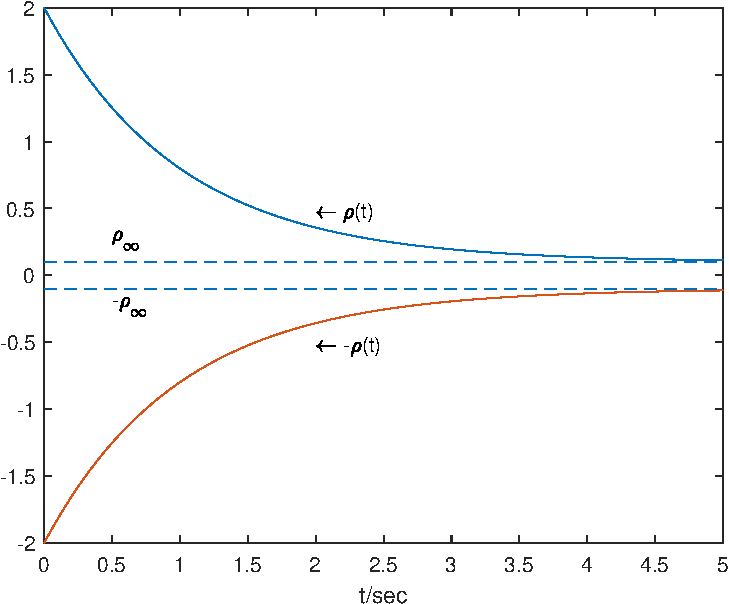
\includegraphics[scale=0.5]{figure/adaptive/p.pdf}
       \captionsetup{hypcap=false}
       \captionof{figure}{上述性能函数的图形($\lambda=1,\rho_0=2,\rho_{\infty}=0.1$)}
   \end{center}
\end{example}
我们欲使$|e(t)|<\rho(t)$,那么通过指定合适的$\rho(t)$,即可限制误差的稳态和瞬态特性。

为了应用之前手段(分析信号的有界性)来分析上述问题,我们引入以下{\bf 误差转换(error transformation)},将上述有约束的跟踪误差变为等价的无约束问题。

具体而言,我们定义\[e(t)=\rho(t)T(\zeta)\]
其中$\zeta$是变换后的无约束误差,$T(\zeta)$是光滑的函数,并具有如下性质:
\begin{itemize}[leftmargin=1em]
    \item $T(\zeta)$严格单调递增;
    \item $\lim\limits_{\zeta\to-\infty}T(\zeta)=-1$,$\lim\limits_{\zeta\to\infty}T(\zeta)=1$。
\end{itemize}
则有
\[\zeta = T^{-1}\left(\frac{e(t)}{\rho(t)}\right)\]
$\frac{e(t)}{\rho(t)}\to -1$时,$\zeta\to-\infty$;$\frac{e(t)}{\rho(t)}\to 1$时,$\zeta\to\infty$。
我们发现,如果$\zeta$有界,那么$-1<\frac{e(t)}{\rho(t)}<1$,这样,分析$\zeta$的有界性就等价于分析误差满足的约束。

\begin{example}
    以下两个$T^{-1}$都是可行的:
    \[\zeta = \tan\left(\frac{\pi}{2}\frac{e(t)}{\rho(t)}\right),\zeta = \ln\left(\frac{e(t)+\rho(t)}{\rho(t)-e(t)}\right)\]
\end{example}

接下来对$\zeta$的动力学进行分析:
\begin{align*}
    \dot{\zeta} &= \frac{\partial T^{-1}}{\partial \left(\frac{e(t)}{\rho(t)}\right)}
    \frac{\diff}{\diff t}\left(\frac{e(t)}{\rho(t)}\right)
\end{align*}
易知第一个因子为正定(因$T^{-1}$随$\left(\frac{e(t)}{\rho(t)}\right)$单调递增),记其为$R$。
则上式等于
\begin{align*}
    \dot{\zeta} &= R
    \frac{\diff}{\diff t}\left(\frac{e(t)}{\rho(t)}\right)\\
    &=R\frac{\dot{e}(t)\rho(t)-e(t)\dot{\rho}(t)}{\rho^2(t)}\\
    &=\frac{R}{\rho(t)}(u+\varphi(x)\theta-\dot{x}_d(t))-\frac{Re(t)\dot{\rho}(t)}{\rho^2(t)}
\end{align*}
可选取\[u=-\varphi(x)\hat{\theta}+\frac{\dot{\rho}(t)}{\rho(t)}e(t)+\dot{x}_d(t)+\frac{\rho(t)}{R}u_0\]
以消去第二项与括号中第三项,得到
\[\dot{\zeta} = u_0-\frac{R}{\rho(t)}\varphi(x)\tilde{\theta}\]
其中$\tilde{\theta}\triangleq \hat{\theta}-\theta$。
于是进一步选取$u_0=-k\zeta,k>0$,有
\[\dot{\zeta} = -k\zeta-\frac{R}{\rho(t)}\varphi(x)\tilde{\theta}\]
考虑如下候选Lyapunov函数
\[V=\frac{1}{2}\zeta^2+\frac{1}{2\gamma}\tilde{\theta}^2,\gamma>0\]
求其导数得\begin{align*}
    \dot{V}&=\zeta\left(-k\zeta-\frac{R}{\rho(t)}\varphi(x)\tilde{\theta}\right)+\frac{1}{\gamma}\tilde{\theta}\dot{\hat{\theta}}\\
    &=-k\zeta^2+\frac{1}{\gamma}\tilde{\theta}\left(\dot{\hat{\theta}}-\gamma \frac{R}{\rho(t)}\varphi(x)\zeta\right)
\end{align*}
设计\[\dot{\hat{\theta}}=\gamma \frac{R}{\rho(t)}\varphi(x)\zeta\]
则$\dot{V}=-k\zeta^2\le 0$,类似 \ref{4Bref} 节各例可分析$\zeta$有界性。进而$|e(t)|<\rho(t)$,达成了我们的目标。

进一步地,如果我们超调量有要求,即要求$e(t)$穿过横轴时的下冲/上冲(具体由$e(0)$的正负而定,即$e(0)$为正时限制下冲,$e(0)$为负时限制上冲)要小,如何考虑该问题?
我们发现,如指定超调小于$\delta\rho(0)$($0\le\delta\le 1$。此为常值,故假定是可行的),则要求$-\delta\rho(t)<e(t)<\rho(t)$(若$e(0)>0$)或$-\rho(t)<e(t)<\delta\rho(t)$(若$e(0)<0$)即可。

类似本节前述思路进行误差转换。定义\[e(t)=\rho(t)T(\zeta)\]
其中$\zeta$是变换后的无约束误差,$T(\zeta)$仍为光滑且单调递增的函数,并且:
\begin{itemize}[leftmargin=1em]
    \item 若$e(0)>0$,则$\lim\limits_{\zeta\to-\infty}T(\zeta)=-\delta$,$\lim\limits_{\zeta\to\infty}T(\zeta)=1$;
    \item 若$e(0)<0$,则$\lim\limits_{\zeta\to-\infty}T(\zeta)=-1$,$\lim\limits_{\zeta\to\infty}T(\zeta)=\delta$。
\end{itemize}

\begin{example}
    以下$T$是可行的:
    \[T(\zeta) = \begin{cases}
        \frac{\mathrm{e}^\zeta-\delta \mathrm{e}^{-\zeta}}{\mathrm{e}^\zeta+ \mathrm{e}^{-\zeta}}&e(0)>0\\
        \frac{\delta\mathrm{e}^\zeta- \mathrm{e}^{-\zeta}}{\mathrm{e}^\zeta+ \mathrm{e}^{-\zeta}}&e(0)<0
    \end{cases}\]
\end{example}
之后类似本节前述思路进行控制器设计,使$\zeta$有界即可。

更一般地,我们可以将上下界取为不同的函数,即
\[\rho_1(t)<e(t)<\rho_2(t)\]
其中$\rho_1(t),\rho_2(t)$都是定义如 \ref{performance_func} 的性能函数。

进行误差转换。定义\[e(t)=T(\zeta,\rho_1(t),\rho_2(t))\]
其中$\zeta$是变换后的无约束误差。
则\[\zeta = T^{-1}(e(t),\rho_1(t),\rho_2(t))\]
因此,我们要求\[\lim\limits_{\zeta\to-\infty}T(\zeta,\rho_1(t),\rho_2(t))=\rho_1(t),\lim\limits_{\zeta\to\infty}T(\zeta,\rho_1(t),\rho_2(t))=\rho_2(t)\]
\begin{example}
    以下$T^{-1}$是可行的:
    \[\zeta = \tan\left(\frac{\pi}{2}\frac{2e(t)-\rho_1(t)-\rho_2(t)}{\rho_2(t)-\rho_1(t)}\right)\]
\end{example}

之后类似本节前述思路进行控制器设计,使$\zeta$有界即可。

\chapter{自适应控制}\label{cp5}
\section{概述}

\subsubsection*{鲁棒控制(略)}

\subsubsection*{增益调整(Gain Scheduling)}
\addcontentsline{toc}{subsubsection}{增益调整(Gain Scheduling)}

\subsubsection*{直接与非直接自适应控制}

\subsubsection*{模型参考自适应控制(Model Reference Adaptive Control,MRAC)}
% \newpage
\section{模型参考自适应控制:示例与方法}

\subsection{引入}

\subsection{}

\subsection{标量系统的非直接型模型参考自适应控制}

\[\dot{x}=ax+bu\]

\[\dot{x}_{ref}=-a_{ref}x_{ref}+b_{ref}u_c,a_ref>0\]

\[\dot{\hat{b}}(t)=\begin{cases}
  \gamma_2ue&\text{若}\ |\hat{b}|>b_{\min}\\
  &\text{或}\ |\hat{b}|=b_{\min}\ \text{且}\ ue\sgn(b)\ge 0\\
  0&\text{其他}
\end{cases}\]

\subsection{多输入多输出(MIMO)系统的直接型模型参考自适应控制}

\begin{equation}\label{MIMO}
  \dot{x}=Ax+B\Lambda u
\end{equation}

其中$x\in\R{}^n$是系统的状态,

\begin{align}
  \dot{e}&=\dot{x}-\dot{x}_{ref}\nonumber\\
  &=A_{ref}e+B\Lambda\tilde{K}_1x+B\Lambda\tilde{K}_2u_c
\end{align}

类比之前的构造,考虑如下“形式上的”Lyapunov函数
\begin{align*}
  V&=\frac12e^2+\frac{1}{2}\tilde{K}_1^2+\frac{1}{2}\tilde{K}_2^2
\end{align*}
由于其中的$e,\tilde{K}_1,\tilde{K}_2$都是向量或矩阵,而Lyapunov函数输出是标量,上述式子要做相应的修改。
首先,将$e^2$换成$e^\mathrm{T}e$;然后,将$\tilde{K}_1^2$换为\[\tr(\tilde{K}_1^\mathrm{T}\tilde{K}_1)\]
由于$\tilde{K}_1^\mathrm{T}\tilde{K}_1$是实对称矩阵,故其一定可做相似对角化,对角化之后的,而迹是相似不变量,

半正定的,;
而迹等于矩阵所有特征值之和,故$\tilde{K}_1\ne0$时,上式一定为正;

\begin{equation}\label{MIMOLYA}
  V=e^\mathrm{T}Pe+\tr(\tilde{K}_1^\mathrm{T}\tilde{K}_1)+\tr(\tilde{K}_2^\mathrm{T}\tilde{K}_2)
\end{equation}

其中$P$是满足如下Lyapunov方程的正定矩阵。求其对$t$的导数可得
\begin{align}
  \dot{V}&=\dot{e}^\mathrm{T}Pe+e^\mathrm{T}P\dot{e}+2\tr(\tilde{K}_1^\mathrm{T}\dot{\tilde{K}}_1)+
  2\tr(\tilde{K}_2^\mathrm{T}\dot{\tilde{K}}_2)\\
  &=\dot{e}^\mathrm{T}(A_{ref}^\mathrm{T}P+PA_{ref})e+2{e}^\mathrm{T}PB\Lambda\tilde{K}_1x+2{e}^\mathrm{T}PB\Lambda
  \tilde{K}_2u_c+2\tr(\tilde{K}_2^\mathrm{T}\dot{\tilde{K}}_2)\\
  &=-e^\mathrm{T}Qe+2\tr(\tilde{K}_1^\mathrm{T}\Lambda B^\mathrm{T}Pex^\mathrm{T})+2\tr(\tilde{K}_2^\mathrm{T}\Lambda B^\mathrm{T}Peu_c^\mathrm{T})+2{e}^\mathrm{T}PB\Lambda\tilde{K}_2u_c+2\tr(\tilde{K}_2^\mathrm{T}\dot{\hat{K}}_2)
\end{align}
其中第三行我们用到了
\begin{align*}
  {e}^\mathrm{T}PB\Lambda\tilde{K}_1x&=\tr({e}^\mathrm{T}PB\Lambda\tilde{K}_1x)&\text{(标量)}\\
  &=\tr(x{e}^\mathrm{T}PB\Lambda\tilde{K}_1)&\text{(}\tr(AB)=\tr(BA)\text{)}\\
  &=\tr(\tilde{K}_1^\mathrm{T}\Lambda B^\mathrm{T}Pex^\mathrm{T})&\text{(}\tr(A^\mathrm{T})=\tr(A)\text{)}
\end{align*}
于是我们可设计

但是该设计是不可行的,

\begin{equation}\label{MODMIMOLYA}
  V=e^\mathrm{T}Pe+\tr(\tilde{K}_1^\mathrm{T}\textcolor{red}{\Lambda}\tilde{K}_1)+\tr(\tilde{K}_2^\mathrm{T}\textcolor{red}{\Lambda}\tilde{K}_2)
\end{equation}


% \input{Chapter_5/Exercises_5A.tex}
% \newpage
\section{反馈线性化}\label{5Bref}
\textbf{基本思想:}若能将非线性的动力学转化为线性的,那么便可采用控制线性系统的手段来控制非线性系统。
\begin{note}
    这和通过(利用雅可比矩阵的)局部线性化完全不同,因为反馈线性化是通过{\bf 精确的}状态变换和反馈全局完成的,而不是通过取动力学的局部线性{\bf 近似}。
\end{note}

{\bf 问题陈述:} 给定$\dot{x} = f (x, u), x \in \mathbf{R}^n, u
  \in \mathbf{R}^m$,求出函数$g, h$、矩阵$A \in \mathbf{R}^{n \times n}, B \in \mathbf{R}^{n\times m}$,以及新变量$z \in
  \mathbf{R}^n, v \in \mathbf{R}^m$,使得
  \begin{align*}
      u &= g (x, v)&\text{{\small(控制输入,将系统本来的控制输入和给线性化状态的控制输入联系起来)}}\\
      z &= h (x),&\text{{\small(原状态与新状态的变换,将原状态与线性化后的新状态联系起来)}}\\
      \dot{z} &= A  z + B  v,&\text{(新状态满足的线性方程)}
  \end{align*}
然后利用控制线性系统的方法来设计$v$。

\subsection{输入到状态线性化}
\begin{example}[可控标准型]
考虑下述系统
    \begin{align*}
    \dot{x}_1 & =  x_2\\
     \dot{x}_2 & =  x_3\\
     \vdots &   \\
     \dot{x}_{n - 1} & = x_n\\
    \dot{x}_n & = f (x) + b (x) u
\end{align*}
假设$b \neq 0$,设计如下控制输入
\[ u = \frac{1}{b (x)} (v - f (x)) \]
则我们可消去非线性项,而得到
$ \dot{x}_n = v $,
这就将系统转化为可控标准型。控制律可选择为
\[ v = - k_0 x_1 - k_1 x_2 - \cdots - k_{n - 1} x_n \]
其中各 $k_i$ 应使得多项式(其实就是线性化后系统的特征多项式)
\[ p^n + k_{n - 1} p^{n - 1} + \cdots + k_0 = 0 \]
的所有根都具有负实部,这样就可使 $x (t) \rightarrow 0$。
\end{example}
\begin{example}[更一般的例子]
  考虑下述系统
  \begin{align*}
    \dot{x}_1 & = - 2 x_1 + a  x_2 + \sin  x_1\\
    \dot{x}_2 & = - x_2 \cos  x_1 + u  \cos (2 x_2)
  \end{align*}
  本例的难点主要在于,第一个方程中的非线性项无法直接被$u$消去。于是,我们寻求状态变换$z = z (x)$与输入变换$u = u (x, v)$使得非线性系统转为线性的。
  
  选取状态变换 $z_1 = x_1, z_2 = a  x_2 + \sin  x_1$,那么 $a  x_2 = z_2 -\sin  z_1$。因此
  \begin{align*}
    \dot{z}_1 & = - 2 z_1 + z_2\\
    \dot{z}_2 & = a  \dot{x}_2 + \cos  x_1 \cdot \dot{x}_1\\
    & = a  (- x_2 \cos  x_1 + u  \cos (2 x_2)) + \cos  x_1 (- 2 x_1 + a 
    x_2 + \sin  x_1)\\
    & = (\sin  x_1 - 2 x_1) \cos  x_1 + u  a   \cos (2 x_2)\\
    & \triangleq f(x)+g(x)u
  \end{align*}
  选取 $u = \frac{1}{g(x)} (v - f(x))$,我们就得到下述线性系统
  \[ \left\{\begin{array}{l}
       \dot{z}_1 = - 2 z_1 + z_2\\
       \dot{z}_2 = v
     \end{array}\right. \]
  该系统是能控的。那么,采用控制律$v = - k_1 z_1 - k_2 z_2$,只要增益$k_1$ 和 $k_2$设置得当,我们就能将极点配置在左半平面任意我们需要的位置上,而镇定这个系统。
  
  \begin{remark}   
    \begin{enumerate}[leftmargin=2em]
      \item 上面获得的结果并非全局的,因为当$g(x)=0$时$u$没有定义。
      
      \item 为了实际应用上述控制律,新状态变量$(z_1,z_2)$必定要能获取。也即,系统的全部状态$(x_1, x_2)$都要可测,才能计算出所需的$u$。
    \end{enumerate}
  \end{remark}
\end{example}

\subsection{输入到输出线性化}

在原系统上增加输出 $y$:
\[ \left\{\begin{array}{l}
     \dot{x} = f (x, u)\\
     y = h (x)
   \end{array}\right. \]
目标是:设计 $u$ 使得$y \rightarrow 0$。我们希望得出 $y$ 与 $u$之间简单而直接的表达式。

\begin{example}
    考虑下述三阶系统
    \begin{align*}
  \dot{x}_1 & = \sin  x_2 + (x_2 + 1) x_3\\
  \dot{x}_2 & = x^2_1 + x_3\\
  \dot{x}_3 & = x^2_2 + u\\
  y & = x_1
\end{align*}
对输出求一阶导数得到
\[ \dot{y} = \dot{x}_1 = \sin  x_2 + (x_2 + 1) x_3 \]
上式仍然不直接与$u$相关,尝试再求一阶导数得到
\begin{align*}
  \ddot{y} & = \dot{x}_2 \cos  x_2 + \dot{x}_2 x_3 + (x_2 + 1) \dot{x}_3\\
  & = (x^2_1 + x_3) \cos  x_2 + x_3 (x^2_1 + x_3) + (x_2 + 1) (x^2_2 + u)\\
  & = (x^2_1 + x_3) (\cos  x_2 + x_3) + (x_2 + 1) x^2_2 + u (x_2 + 1)\\
  & \triangleq  f(x) + g(x)u
\end{align*}
设计 \[u = \frac{1}{g(x)} (v - f (x))\]
我们就有 $\ddot{y} = v$。此时就可用设计线性系统的方法,设计 $v = - k_1 y - k_2 \dot{y},k_1,k_2>0$,即可使输出$y$稳定(提示:二阶微分方程$\ddot{y}+k_2 \dot{y}+k_1 y=0$的特征根具有负实部)。
\end{example}

\begin{remark}  
    这种方法的缺陷:
  \begin{enumerate}
    \item 需要得知所有的状态$(x_1, x_2, x_3)$才可计算控制$u$。
    
    \item $g(x)=0$,即$x_2 = - 1$时,$u$无法应用,即存在奇异点!
    
    \item $y$稳定了,但$x_2, x_3$ 未必稳定?
    \item 并不对所有非线性系统都适用。
  \end{enumerate}
\end{remark}

反馈线性化的基本思想,是将系统中的非线性项消去。然而,我们应该审慎考虑这一思想——{\bf 消去非线性项总是有利的吗}?

\begin{example}
考虑下述系统
    \[\dot{x} = a  x - x^3 + u\]
如果用反馈线性化的思想,那么应设计\[u=-ax+x^3+v\]
这样$\dot{x}=v$,利用$v=-kx,k>0$可镇定原系统。然而,如果一开始$x$离原点较远,$u$可能很大,即控制代价较大。

如果我们简单设计$u=-ax$,那么$\dot{x}=-x^3$,很容易看出系统已然渐近稳定。

因此,就像 \ref{1Aref} 节所说的那样,有些非线性对系统的运行是有害的,应设法克服它的有害影响;有些非线性是有益的,应在设计时予以考虑。后续章节的一些方法就会充分考虑这些有利因素(如 \ref{5Dref} 节要介绍的反步法)。
\end{example}

% \input{Chapter_5/Exercises_5B.tex}
% \newpage
\newpage
\section{滑模控制(Sliding mode control)}\label{5Cref}

\subsection{引入:镇定问题}

 考虑如下二阶系统
 \begin{equation}
   \begin{aligned}
    \dot{x}_1 & = x_2\\
       \dot{x_2} & = f (x) + g (x) u
    \end{aligned}\label{Sys:sliding_mode}
 \end{equation}
  其中$f (x)$和$g (x)$都是非线性函数,$g (x) \geq g_0 > 0$,
  
  对于镇定问题,我们的\textbf{控制目标:}设计$u$以镇定原点,也就是使$t
  \rightarrow \infty $时$ x_1, x_2 \rightarrow 0$。
  
  基本思想是,定义一\textbf{滑模面(sliding surface)}\[s = x_2 + \lambda x_1 = 0,
  \lambda > 0\]
  在该面上, \[ s = 0 \Rightarrow \left\{\begin{array}{l}
       \dot{x}_1 = - \lambda x_1 \Rightarrow x_1 (t) = x_1 (0) \mathrm{e}^{- \lambda t}\\
       x_2 = - \lambda x_1 = - \lambda x_1 (0) \mathrm{e}^{- \lambda  t}
     \end{array}\right. \]
     也就是说,一旦系统状态能够在有限时间内到达此滑模面,此后系统状态就能以指定速率收敛。
  
  因此,一般的滑模控制过程可分为两阶段:
  
  \textbf{1. 接近阶段:}设计$u$,迫使$x_1, x_2$这些状态在有限时间内到达所设计的滑模面。
  
  \textbf{2. 滑模阶段:}$x_1, x_2$在滑模面上到达原点。
  
  接下来设计接近阶段控制律。要让$s\to 0$,考虑候选Lyapunov函数\[V = \frac{1}{2} s^2\]
  求其导数得
  \[ \dot{V} = s \cdot \dot{s}=s(\dot{x}_2 + \lambda \dot{x}_1) = s (f (x) + g (x) u + \lambda x_2) \]
  设计\[u = \frac{1}{g (x)} (- f (x) - \lambda x_2 - k \sgn (s)),k > 0,\ensuremath{\operatorname{sgn}}(s) = \left\{\begin{array}{ll}
  1 & s > 0\\
  0 & s = 0\\
  - 1 & s < 0
\end{array}\right.\]
  则$\dot{s} = - k \sgn (s)$,称其为\textbf{等速趋近律}。
  若希望$s$较大时减小较快,亦可设计$u$使得$\dot{s}
  = - k \sgn (s) - k_1 s,k,k_1>0$,这称为\textbf{指数趋近律}。
  
  按上述等速趋近律,可得$\dot{V} = - ks \sgn (s) = - k | s | =
  - k \sqrt{2 V}$,即$\frac{\dot{V}}{\sqrt{V}} = - \sqrt{2} k $。两边积分得到
  \[ \int^t_0 \frac{\dot{V}}{\sqrt{V}} \diff t = 2 \left. \sqrt{V} \right|^t_0 = 2
   \sqrt{V (t)} - 2 \sqrt{V (0)}  = - \sqrt{2} k  t \]
  
  因此,当$t \geq \frac{\sqrt{2 V (0)}}{k}$时,$V (t) \equiv 0$,即在有限时间内,$s (t) \equiv 0$。

  \begin{note}
    若将上述的$-k\sgn(s)$换成$-ks$,则$\dot{V} = - ks^2=  - 2k V$,类似上面方法可得同样的结论。注意,在 \ref{5C3ref} 小节中此替换不再成立(可考虑:接近原点时$s$很小,不能克服干扰,但$\sgn(s)$能保持原值)。
  \end{note}

  进而,将$s = x_2 + \lambda x_1 = \dot{x}_1 + \lambda x_1$写成
  \[ \dot{x}_1 = - \lambda x_1 + s \]
  这样$x_1$ 可视为状态,$s$ 可视为控制输入。
  注意到无外力系统(不含输入)的原点为指数稳定。于是,由输入-状态稳定性(引理 \ref{ISS_lemma}),我们有$s \rightarrow 0 \Rightarrow x_1 \rightarrow 0, x_2 \rightarrow 0$。

\subsection{推广到跟踪问题}

仍考虑系统 \eqref{Sys:sliding_mode}。
现在,我们的{\bf 控制目标}是:$(x_1, x_2) \rightarrow (x_d, \dot{x}_d)$。

定义跟踪误差$\tilde{x}_1 = x_1 - x_d$,$\tilde{x}_2 = x_2 - \dot{x}_d$,
设计滑模面\[s = \tilde{x}_2 + \lambda \tilde{x}_1 = 0,\lambda>0\]
则$s$的动力学
\begin{align*}
\dot{s} &= \dot{\tilde{x}}_2 + \dot{\tilde{x}}_1 \lambda \\
&= \dot{x}_2 -\ddot{x}_d (t) + \lambda \dot{\tilde{x}}_1 \\
&= f (x) + g (x) u - \ddot{x}_d (t) +\lambda \tilde{x}_2
\end{align*}

考虑候选Lyapunov函数$V = \frac{1}{2} s^2$,求其导数得
\[\dot{V} = s \cdot \dot{s} = s (f (x) + g (x) u -
\ddot{x}_d (t) + \lambda \tilde{x}_2)\]

于是设计\begin{equation}
    u = \frac{1}{g (x)} (- f (x) + \ddot{x}_d (t) - \lambda \tilde{x}_2 - k
\sgn (s)),k>0\label{tracking_control}
\end{equation}这样$\dot{s} = - k \sgn (s)$,$\dot{V}=-k|s|$。后续分析同上小节。

\subsection{推广到有不确定性的跟踪问题}\label{5C3ref}
仍考虑系统 \eqref{Sys:sliding_mode}。现在,函数 $f (x)$ 不再已知,但其可由估计$\hat{f} (x)$ 和误差限 $F (x)$表征:
\[ | \hat{f} (x) - f (x) | \leq F (x) \]
函数 $g (x)$ 未知,其界为 $0 < g_{\min} (x) \leq g (x) \leq g_{\max}(x)$。

定义 $\hat{g} (x) = \sqrt{g_{\min} (x) g_{\max} (x)}$,我们有
\[ \frac{1}{\beta} \triangleq \frac{\sqrt{g_{\min} (x) g_{\max}
   (x)}}{g_{\max} (x)} \leq \frac{\hat{g} (x)}{g (x)} \leq
   \frac{\sqrt{g_{\min} (x) g_{\max} (x)}}{g_{\min} (x)} =
   \sqrt{\frac{g_{\max} (x)}{g_{\min} (x)}} \triangleq \beta \geq 1 \]
类似 \eqref{tracking_control},设计$u = \frac{1}{\hat{g} (x)} (- \hat{f} (x) + \ddot{x}_d (t) - \lambda
\tilde{x}_2 - k  \ensuremath{\operatorname{sgn}} (s))$, $k > 0$,仍考虑$V=\frac12 s^2$,求导得到
\begin{align*}
  \dot{V} & = s \left\{ f (x) - \ddot{x}_d (t) + \lambda \tilde{x}_2 +
  \frac{g (x)}{\hat{g} (x)} [- \hat{f} (x) + \ddot{x}_d (t) - \lambda
  \tilde{x}_2 - k  \ensuremath{\operatorname{sgn}} (s)] \right\}\\
  & = s \left\{ [f (x) - \hat{f} (x)] + \left( \frac{g (x)}{\hat{g} (x)} -
  1 \right) (- \hat{f} (x) + \ddot{x}_d (t) - \lambda \tilde{x}_2) - k \frac{g
  (x)}{\hat{g} (x)}  \ensuremath{\operatorname{sgn}} (s) \right\}\\
  & \leq | s | \left\{ F (x) + \left| \frac{g (x)}{\hat{g} (x)} - 1 \right|
  \cdot | - \hat{f} (x) + \ddot{x}_d (t) - \lambda \tilde{x}_2 | - k \frac{g
  (x)}{\hat{g} (x)} \right\}\\
  & = - | s | \left\{ k \frac{g (x)}{\hat{g} (x)} - F (x) - \left| \frac{g
  (x)}{\hat{g} (x)} - 1 \right| \cdot | - \hat{f} (x) + \ddot{x}_d (t) -
  \lambda \tilde{x}_2 | \right\}
\end{align*}
于是可设计 $k$使得
\[ k \frac{g (x)}{\hat{g} (x)} \geq F (x) + \left| \frac{g (x)}{\hat{g} (x)} -
   1 \right| \cdot | - \hat{f} (x) + \ddot{x}_d (t) - \lambda \tilde{x}_2 | +
   \eta, \eta > 0 \]
\[ k \geq \frac{\hat{g} (x)}{g (x)} [F (x) + \eta] + \left| 1 - \frac{\hat{g}
   (x)}{g (x)} \right| \cdot | - \hat{f} (x) + \ddot{x}_d (t) - \lambda
   \tilde{x}_2 | \]
注意到 $\frac{1}{\beta} \leq \frac{\hat{g} (x)}{g (x)} \leq \beta, \beta >1$,
可知$ \frac1\beta -1\le \frac{\hat{g}(x)}{g (x)}-1 \le\beta-1 $,则\[\left|  \frac{\hat{g}
   (x)}{g (x)}-1 \right|=\max\{\beta-1,1-\frac{1}{\beta}\}=\max\{\beta-1,\frac{\beta-1}{\beta}\}=\beta-1\]
则取 $k = \beta [F (x) + \eta] + (\beta - 1) \cdot | - \hat{f} (x) +\ddot{x}_d (t) - \lambda \tilde{x}_2 |$,就有 $\dot{V} \leq - \eta | s|$。后续分析同前两小节。
\subsection{有外部干扰的系统设计}
\noindent\textbf{一、干扰上界已知的情形}

\enlargethispage{1em}
考虑下述系统
 \begin{equation}
      \begin{aligned}
    \dot{x}_1 & = x_2\\
    \dot{x}_2 & = u + d (t)
  \end{aligned}\label{Sys:dis_with_upperbound}
 \end{equation}
  其中 $d (t)$ 是外部干扰,有 $| d (t) | \leq d_{\max}$.
  
  设计滑模面 $s = x_2 + \lambda x_1=0, \lambda > 0$,$s$的动力学是 $\dot{s} = \dot{x}_2 + \lambda \dot{x}_1 = u + d (t)
  + \lambda x_2$。
  
  仍选取候选 Lyapunov 函数为$V = \frac{1}{2} s^2$,求其导数得 $\dot{V} = s \cdot \dot{s} = s (u + d (t) + \lambda x_2)$。
  
  设计 $u = - \lambda x_2 - k  \ensuremath{\operatorname{sgn}} (s)$, $k >
  0$即得到
  \begin{align*}
    \dot{V} & = s (d (t) - k  \ensuremath{\operatorname{sgn}} (s))\\
    & = - k  | s | + s  d (t)\\
    & \leq - (k - d_{\max})  | s |
  \end{align*}
  选取 $k = d_{\max} + \eta, \eta > 0$,即得 $\dot{V} \leq - \eta | s |$。

\noindent\textbf{二、干扰上界未知的情形(1)}

  仍考虑系统 \eqref{Sys:dis_with_upperbound}。若 $d_{\max}$ 是未知的,则可以设计(其中$\hat{k}$是对$k$真值的估计)
  \[ u = - \lambda x_2 - \hat{k} \ensuremath{\operatorname{sgn}} (s) \]
  
  定义 $\tilde{k} = \hat{k} - d_{\max} - \eta$(与上述第一种情况联系起来:$k$的真值可视作$d_{\max}+\eta$)。
  
  考虑如下候选Lyapunov函数
  \[ V = \frac{1}{2} s^2 + \frac{1}{2 \gamma} \tilde{k}^2, \gamma > 0, \]
  求其导数得(注意第三行凑出误差$\tilde{k}$的形式)
  \begin{align*}
    \dot{V} & = s  \dot{s} + \frac{1}{\gamma} \tilde{k} \dot{\hat{k}}\\
    & \leq - (\hat{k} - d_{\max}) | s | + \frac{1}{\gamma} \tilde{k}
    \dot{\hat{k}}\\
    & = - (\hat{k} - d_{\max} - \eta) | s | - \eta | s | + \frac{1}{\gamma}
    \tilde{k} \dot{\hat{k}}\\
    & = \frac{1}{\gamma} \tilde{k} (\dot{\hat{k}} - \gamma | s |) - \eta | s |
  \end{align*}
  设计 $\dot{\hat{k}} = \gamma | s |$,即得 $\dot{V} \leq - \eta | s |$。两边积分得到
  \[ V (t) - V (0) \leq - \eta \int^t_0 | s(\tau) | \diff \tau \]
  因此 $s \in \mathbf{L}_1$。
  则$s \in \mathbf{L}_1 \cap \mathbf{L}_{\infty}, \dot{s} \in
  \mathbf{L}_{\infty}$,根据推论 \ref{barbalat_cor_2},有 $\lim\limits_{t \rightarrow \infty} s = 0$。

\noindent\textbf{三、干扰上界未知的情形(2)}

仍考虑系统 \eqref{Sys:dis_with_upperbound}。干扰$d(t)$满足
  \[ \| d (t) \| \leq d_{\max} (1 + \| x_1 \| + \| x_2 \|^2) \]
并且$d_{\max}$未知。

定义$\Phi(x)=1 + \| x_1 \| + \| x_2 \|^2\ge 1$。
设计滑模面$s = x_2 + \lambda x_1 = 0,  \lambda > 0$,$s$的动力学是 $\dot{s} = \dot{x}_2 + \lambda \dot{x}_1 = u + d (t)
  + \lambda x_2$。

可以设计(其中$\hat{k}$是对$k$的估计。注意,只能估计$d_{\max}$(常值),而不能估计含各状态的乘积项;最后一项的作用类似于之前$\tilde{k}$中的$\eta$)
  \[ u = - \lambda x_2 - \hat{k}\Phi(x) \ensuremath{\operatorname{sgn}} (s) -\eta\sgn(s)\]
这样,$s$的动力学就变为$\dot{s}=d(t)-\hat{k}\Phi(x) \ensuremath{\operatorname{sgn}} (s)-\eta\sgn(s)$。

定义$\tilde{k}=\hat{k}-d_{\max}-\eta\sgn(s)$。考虑如下候选Lyapunov函数
  \[ V = \frac{1}{2} s^2 + \frac{1}{2 \gamma} \tilde{k}^2, \gamma > 0, \]
  求其导数得(注意第三行凑出误差$\tilde{k}$的形式)
  \begin{align*}
    \dot{V} & = s  \dot{s} + \frac{1}{\gamma} \tilde{k} \dot{\hat{k}}\\
    &=s(d(t)-\hat{k}\Phi(x)\sgn(s)-\eta\sgn(s))+\frac{1}{\gamma} \tilde{k} \dot{\hat{k}}\\
    & \leq d_{\max}\Phi(x)|s|-\hat{k}\Phi(x)|s|-\eta|s|+\frac{1}{\gamma} \tilde{k} \dot{\hat{k}}\\
    & = -|s|\Phi(x)\tilde{k}+\frac{1}{\gamma} \tilde{k} \dot{\hat{k}}-\eta|s|\\
    &= \frac{1}{\gamma}\tilde{k} (\dot{\hat{k}}-\gamma |s|\Phi(x))-\eta|s|
  \end{align*}
则取$\dot{\hat{k}}=\gamma |s|\Phi(x)$,就有$\dot{V}=-\eta|s|$,之后的分析同上。

\noindent\textbf{四、干扰上界未知且有不确定性的情形:修正设计}

考虑以下标量系统
\begin{equation}
    \dot{x} = u + \varphi(x)\theta + d(t)
\end{equation}
其中$x$为状态,$u$为控制输入,$\varphi$是连续且已知的函数,$\theta$是未知常数,且$d(t)$是有界且时变的扰动,满足$|d(t)|\le d_{\max}$,$d_{\max}$未知。

类似上述滑模控制的思想(可认为滑模面为$s=x$),考虑设计控制律\[u=-kx-\varphi(x)\hat{\theta}-\hat{k}\sgn(x)\]
并作候选Lyapunov函数\[V=\frac{1}{2}x^2+\frac{1}{2\gamma_1}(\hat{\theta}-\theta)^2+\frac{1}{2\gamma_2}(\hat{k}-d_{\max}-\eta)^2,\gamma_1>0,\gamma_2>0\]
定义$\tilde{\theta}=\hat{\theta}-\theta,\tilde{k}=\hat{k}-d_{\max}-\eta$。求导数得
\begin{align*}
    \dot{V}&=x(-kx-\varphi\tilde{\theta}-\hat{k}\sgn(x)+d(t))+\frac{1}{\gamma_1}\tilde{\theta}\dot{\hat{\theta}}+\frac{1}{\gamma_2}\tilde{k}\dot{\hat{k}}\\
    &\leq -kx^2-\varphi\tilde{\theta}x-\hat{k}|x|+d_{\max}|x|+\eta|x|-\eta|x|+\frac{1}{\gamma_1}\tilde{\theta}\dot{\hat{\theta}}+\frac{1}{\gamma_2}\tilde{k}\dot{\hat{k}}\\
    &=-kx^2+\frac{1}{\gamma_1}\tilde{\theta}(\dot{\hat{\theta}}-\gamma_1\varphi x)+\frac{1}{\gamma_2}\tilde{k}(\dot{\hat{k}}-\gamma_2|x|)-\eta|x|
\end{align*}
于是,只需设计$\dot{\hat{\theta}}=\gamma_1\varphi x$和$\dot{\hat{k}}=\gamma_2|x|$,可以使系统状态在有限时间内趋近于$0$。

上述设计固然可行,但是其在$x=0$附近会存在较明显的振荡。
为了避免$\sgn(x)$的弊端,有学者提出了如下控制律
\[u=-kx-\varphi(x)\hat{\theta}-\textcolor{red}{\frac{\hat{k}^2}{|x|\hat{k}+\mathrm{e}^{-t}}x}\]
这样,$x$的动力学就可写为
\[\dot{x}=-kx-\varphi(x)(\hat{\theta}-\theta)-\frac{\hat{k}^2}{|x|\hat{k}+\mathrm{e}^{-t}}x+d(t)\]
考虑候选Lyapunov函数
\[V=\frac{1}{2}x^2+\frac{1}{2\gamma_1}(\hat{\theta}-\theta)^2+\frac{1}{2\gamma_2}(\hat{k}-d_{\max})^2,\gamma_1>0,\gamma_2>0\]
定义$\tilde{\theta}=\hat{\theta}-\theta,\tilde{k}=\hat{k}-d_{\max}$。求其导数得
\begin{align*}
    \dot{V}&=x\left(-kx-\varphi(x)\tilde{\theta}-\frac{\hat{k}^2}{|x|\hat{k}+\mathrm{e}^{-t}}x+d(t)\right)+\frac{1}{\gamma_1}\tilde{\theta}\dot{\hat{\theta}}+\frac{1}{\gamma_2}\tilde{k}\dot{\hat{k}}\\
    &=-kx^2-x\varphi\tilde{\theta}-\frac{\hat{k}^2}{|x|\hat{k}+\mathrm{e}^{-t}}x^2+d(t)x+\frac{1}{\gamma_1}\tilde{\theta}\dot{\hat{\theta}}+\frac{1}{\gamma_2}\tilde{k}\dot{\hat{k}}\\
    &=-kx^2-\frac{\hat{k}^2}{|x|\hat{k}+\mathrm{e}^{-t}}x^2+d(t)x+\frac{1}{\gamma_1}\tilde{\theta}(\dot{\hat{\theta}}-\gamma_1\varphi x)+\frac{1}{\gamma_2}\tilde{k}\dot{\hat{k}}
\end{align*}
在此步骤,设计$\dot{\hat{\theta}}=\gamma_1\varphi x$以消去其中一项,则($x^2=|x|^2$)
\begin{align*}
    \dot{V}&\leq -kx^2+\frac{1}{\gamma_2}\tilde{k}\dot{\hat{k}}+d_{\max}|x|-\frac{\hat{k}^2}{|x|\hat{k}+\mathrm{e}^{-t}}|x|^2
\end{align*}
仍选取$\dot{\hat{k}}=\gamma_2 |x|$,则
\begin{align*}
   \dot{V} &=-kx^2+{\hat{k}}|x|-\frac{\hat{k}^2}{|x|\hat{k}+\mathrm{e}^{-t}}|x|^2\\
    &=-kx^2+\frac{\hat{k}^2|x|^2+\mathrm{e}^{-t}\hat{k}|x|-\hat{k}^2|x|^2}{|x|\hat{k}+\mathrm{e}^{-t}}\\
    &=-kx^2+\frac{\mathrm{e}^{-t}\hat{k}|x|}{|x|\hat{k}+\mathrm{e}^{-t}}\\
    &\leq -kx^2+\mathrm{e}^{-t}
\end{align*}
对上式两边积分并移项得:
\[V(t)+k\int_{0}^{t} x^2(\tau)\diff\tau\le V(0)+\int_{0}^{t} \mathrm{e}^{-\tau}\diff\tau=V(0)+(1-\mathrm{e}^{-t})\]
可知$V\in\mathbf{L}_\infty,x\in\mathbf{L}_2$,进而$x,\tilde{\theta},\tilde{k},\hat{k},\hat{\theta}\in\mathbf{L}_\infty$,从而$\dot{x}\in\mathbf{L}_\infty$。进而由 \ref{barbalat_cor_1},我们知道$\lim\limits_{t\to\infty}x(t)=0$。
% \input{Chapter_5/Exercises_5C.tex}
% \newpage
\section{反步法(Backstepping)}\label{5Dref}
\subsection{基本反步法}
考虑系统
\begin{equation}
    \begin{aligned}
  \dot{z} & = f (z) + g (z) \xi\\
  \dot{\xi} & = u
\end{aligned}\label{Sys:backstep:basic:original}
\end{equation}
其中 $[z^\mathrm{T}, \xi^\mathrm{T}]^\mathrm{T} \in \mathbb{R}^{n + 1}$ 为状态,$u \in
\mathbb{R}$ 为控制输入。函数$f, g$在包含$z = 0$的域$D$上光滑,且有 $f (0) = 0$。

我们的目标是设计状态反馈控制律以镇定原点。%将原系统看作两个系统之级联。

假设我们能通过一反馈控制律$\xi = \Phi (z)$($\Phi (0) = 0$)来渐近镇定{\bf 第一个系统}(将$\xi$看作虚拟的控制输入),也就是使
\begin{equation}
    \dot{z} = f (z) + g (z) \Phi (z) \label{first_stablize}
\end{equation}
的原点是渐近稳定的。于是,我们可知一定存在 Lyapunov 函数 $V (z)$ 使得
\[ \dot{V} = \frac{\partial V}{\partial z} [f (z) + g (z) \Phi (z)] \leq -
   \omega (z) \]
其中 $\omega (z)$ 正定。

在原系统中加减$g (z) \Phi (z)$,凑出 \eqref{first_stablize} 的形式
\begin{equation}
   \begin{aligned}
  \dot{z} & = f (z) + g (z) \Phi (z) + g (z) (\xi - \Phi (z))\\
  \dot{\xi} & = u
\end{aligned} \label{Sys:backstep:basic:control}
\end{equation}

引入状态变换(表征“真实的”$\xi$和“理想的”$\xi=\Phi (z)$之间的差异)
\[ y = \xi - \Phi (z) \]
这样,我们如果让$y\to 0$,那么$\xi$就能跟踪理想的控制律$\Phi$,$z$也按上面原点渐近稳定的系统之规律变化。
于是,原系统变为
\begin{equation}
    \begin{aligned}
  \dot{z} & = f (z) + g (z) \Phi (z) + g (z) y\\
  \dot{y} & = \dot{\xi}-\dot{\Phi} (z) = u - \dot{\Phi} (z)
\end{aligned}\label{Sys:backstep:basic:backstep}
\end{equation}
此种状态变换常称作 {\textbf{反步法(backstepping)}}\index{反步法(backstepping)},因为它将控制$- \Phi (z)$“反挪”(back-steps)到了积分之前。

\begin{figure}[htbp]
    \centering
    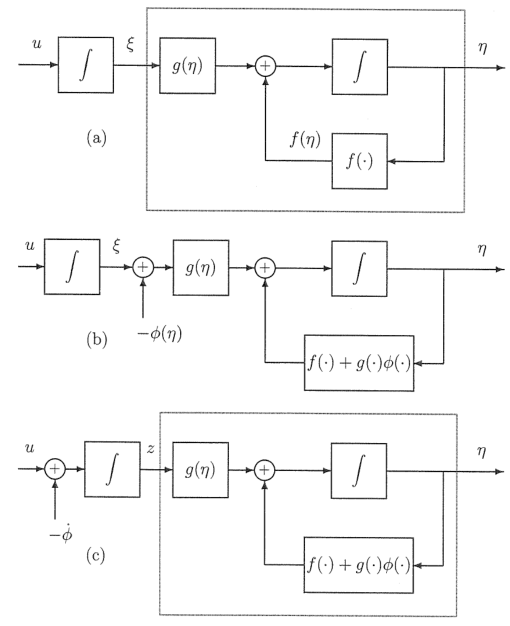
\includegraphics[width=0.5\linewidth]{figure/adaptive/backstepping.png}
    \caption{反步法示意图。图中的$\eta$为此处的$z$,$z$为此处的$y$。(a) 原系统 \eqref{Sys:backstep:basic:original};(b) 引入控制$\Phi(z)$,即 \eqref{Sys:backstep:basic:control};(c) 将$\Phi(z)$“反挪”(back-steps)到积分之前,即 \eqref{Sys:backstep:basic:backstep}。}
    \label{fig:backstepping}
\end{figure}

因为 $f, g$ 与 $\Phi$ 已知,所以可求出
\[ \dot{\Phi} (z) = \frac{\partial \Phi}{\partial z} \dot{z} = \frac{\partial
   \Phi}{\partial z} (f (z) + g (z) \xi) \]
令 $v = u - \dot{\Phi} (z)$(“新的”控制输入),将上述系统简化成
\begin{align*}
  \dot{z} & = f (z) + g (z) \Phi (z) + g (z) y\\
  \dot{y} & = v
\end{align*}
% 这与我们一开始讨论的系统形式大体相同,当$y=0$时第一式中多余的项消失,$z$的原点便渐近稳定。which has the same ``form'' as the system we started with the exception that
% we know the first component is asymptotically stable at the origin when $y$ is zero.

考虑如下候选的合并Lyapunov 函数(combined Lyapunov function candidate,意即将新状态合并进来)
\[ V_c (z, y) = V (z) + \frac{1}{2} y^2 \]
求其导数得
\begin{align*}
  \dot{V}_c (z, y) & = V (z) + y \cdot \dot{y}\\
  & = \frac{\partial V}{\partial z} [f (z) + g (z) \Phi (z) + g (z) y] + y 
  v\\
  & \leq - \omega (z) + \frac{\partial V}{\partial z} g (z) y + y  v
\end{align*}
则取 \[v = - \frac{\partial V}{\partial z} g (z) - k  y, k > 0\]
即可得到\[\dot{V} (z, y) \leq - \omega (z) - k  y^2\]
它是负定的,
这也就表明上述系统的原点 $(z = 0, y = 0)$ 是渐近稳定的。因为
$\Phi (0) = 0$,所以$z = 0, y = 0\implies \xi =0$,即原系统的原点$(z = 0, \xi = 0)$ 是渐近稳定的。整理得到反馈控制律为
\begin{align*}
  u & = v + \dot{\Phi}(z)\\
  & = - \frac{\partial V}{\partial z} g (z) - k  y + \frac{\partial
  \Phi}{\partial z} (f (z) + g (z) \xi)\\
  & = - \frac{\partial V}{\partial z} g (z) - k  (\xi - \Phi (z)) +
  \frac{\partial \Phi}{\partial z} (f (z) + g (z) \xi)
\end{align*}
\begin{example}[利用反步法进行非线性系统设计]
  考虑下述系统
  \begin{align*}
    \dot{x}_1 & = x^2_1 - x^3_1 + x_2\\
    \dot{x}_2 & = u
  \end{align*}
 首先考虑第一个方程,这时将 $x_2$ 视为虚拟的控制输入,先设计反馈控制律 $\Phi (x_1)$(虚拟的$x_2$) 来镇定 $x_1 = 0$。
  
  设计 $\Phi (x_1) = - x^2_1$,我们有 $\dot{x}_1 = - x^3_1$(将稳定的$- x^3_1$保留)。这样就渐近镇定了第一个系统。
  
  下面应用反步法。选取状态变换(“真实的”$x_2$和“理想的”$x_2$之间的差异)
  \[ y = x_2 - \Phi (x_1) = x_2 + x^2_1 \]
  那么原系统可写为下述形式
  \begin{align*}
    \dot{x}_1 & = - x^3_1 + y\\
    \dot{y}  & = v
  \end{align*}
  其中 $v = u + 2 x_1 (x^2_1 - x^3_1 + x_2)$。
  
  接下来,我们考虑如下候选合并Lyapunov 函数
  \[ V_c = \frac{1}{2} x^2_1 + \frac{1}{2} y^2 \]
  其导数为
  \begin{align*}
    \dot{V}_c & = x_1 \dot{x}_1 + y  \dot{y} = - x^4_1 + x_1 y + y  v
  \end{align*}
  选取 $v = - x_1 - k  y, k > 0$,那么 $\dot{V}_c = - x^4_1 - k  y^2$ 负定。
  因此, $x_1, y \rightarrow 0$,也就说明$x_1,x_2\rightarrow 0$。
  
  整理得控制输入如下
  \[ u = v - 2 x_1 (x^2_1 - x^3_1 + x_2) = - x_1 - k  y - 2 x_1 (x^2_1 - x^3_1
     + x_2) \]
\end{example}

\begin{problem}\label{Pro:backstep-complex}
如果系统不是由二个系统级联
    \begin{align*}
    \dot{x}_1 & = x^2_1 - x^3_1 + x_2\\
    \dot{x}_2 & = - x^2_1 + x_1 x_2 + \cdots \\
    \dot{x}_3 & = u
  \end{align*}
  甚或并不存在$\dot{x}_i=u$的项,比如
  \begin{align*}
    \dot{x}_1 & = -x_1^3+ x_2+\sin x_1\\
    \dot{x}_2 & = \cos x_2-x_2^2 + x_3 \\
    \dot{x}_3 & = u +\cos x_1 +x_2^2
  \end{align*}
  如何进行设计?
\end{problem}

\subsection{自适应反步法}

考虑如下系统
\begin{equation}
    \begin{aligned}
  \dot{x}_1 & = x_2 + \varphi (x_1) \theta\\
  \dot{x}_2 & = u
\end{aligned}\label{Sys:adaptive_backstepping}
\end{equation}
其中 $\theta$ 为未知常数,$\varphi (x_1)$ 是有界函数,$\varphi (0) = 0$。

不妨假设 $\theta$ 已知。若将$x_2$看作控制输入,理想情况下其应设计为
\[- k_1 x_1 - \varphi (x_1) \theta \triangleq \alpha_1 (x_1,\theta), k_1 > 0
\]
但是, $\theta$ 未知。不过,引入自适应控制思想,仍可应用反步法。\index{反步法(backstepping)!自适应$\sim$}

\noindent{\textbf{步骤 1: }}

定义 $z_1 = x_1$,将$x_2$看作控制输入。因为$\theta$ 未知,设计自适应律($v_1$即 $\theta$的状态估计$\hat{\theta}$)
\begin{align*}
  \alpha_1 (x_1, v_1) & = - k_1 z_1 - \varphi (z_1) v_1
\end{align*}
并定义状态变换(“真实的”$x_2$减去“理想的”$x_2$)
\[ z_2 \triangleq x_2 - \alpha_1 (x_1, v_1) \]
于是$z_1$的动力学写为
\begin{align*}
  \dot{z}_1 & = \dot{x}_1\\
  & = x_2 + \varphi (z_1) \theta\\
  & = x_2 - \alpha_1 (x_1, v_1) + \alpha_1 (x_1, v_1) + \varphi (z_1)
  \theta\\
  & = z_2 - k_1 z_1 - \varphi (z_1) (v_1 - \theta)
\end{align*}
考虑如下候选 Lyapunov 函数(欲使$x_1$与参数估计误差趋于$0$)
\[ V_1 (z_1, v_1) = \frac{1}{2} z^2_1 + \frac{1}{2 \gamma_1} (v_1 - \theta)^2
\]
求其导数得到
\begin{align*}
  \dot{V}_1 & = z_1 \dot{z}_1 + \frac{1}{\gamma_1} (v_1 - \theta)
  \dot{v}_1\\
  & = z_1 (z_2 - k_1 z_1 - \varphi (z_1) (v_1 - \theta)) +
  \frac{1}{\gamma_1} (v_1 - \theta) \dot{v}_1\\
  & = -k_1z_1^2+z_1z_2+\frac{1}{\gamma_1} (v_1-\theta)(-\gamma_1z_1\varphi (z_1) +\dot{v}_1)
\end{align*}
设计
\[\dot{v}_1 = \gamma_1 z_1 \varphi (z_1)\]
则
\begin{align*}
  \dot{V}_1 &  = - k_1 z^2_1 + z_1 z_2
\end{align*}

\noindent{\textbf{步骤 2: }}

$z_2$的动力学写为
  \begin{align*}
  \dot{z}_2 & = \dot{x}_2 - \dot{\alpha}_1 (z_1, v_1)\\
  & = u - \frac{\partial \alpha_1}{\partial z_1} \dot{z}_1 - \frac{\partial
  \alpha_1}{\partial v_1} \dot{v}_1\\
  & = u - \frac{\partial \alpha_1}{\partial z_1} (x_2 + \varphi (z_1)
  \theta) - \frac{\partial \alpha_1}{\partial v_1} \gamma_1 z_1 \varphi
  (z_1)\\
  & = u - \frac{\partial \alpha_1}{\partial z_1} x_2 - \frac{\partial
  \alpha_1}{\partial v_1} \gamma_1 z_1 \varphi (z_1) - \theta \frac{\partial
  \alpha_1}{\partial z_1} \varphi (z_1)
\end{align*}
接下来,我们尝试选取一候选Lyapunov函数并设计$u$,使得闭环系统是渐近稳定的。
首先尝试考察下列候选合并Lyapunov函数(为何是“尝试”?请注意上式中含有的未知参数$\theta$)
\[ V_c (z_1, z_2, v_1) = V_1 (z_1, v_1) + \frac{1}{2} z^2_2 \]
求其导数得
\begin{align*}
  \dot{V}_c & = \dot{V}_1 + z_2 \dot{z}_2\\
  & = - k_1 z^2_1 + \textcolor{third}{z_1 z_2} + z_2 \left( u \textcolor{structurecolor}{- \frac{\partial
  \alpha_1}{\partial z_1} x_2 - \frac{\partial \alpha_1}{\partial v_1}
  \gamma_1 z_1 \varphi (z_1)} \textcolor{second}{- \theta \frac{\partial \alpha_1}{\partial z_1}  \varphi (z_1)} \right)
\end{align*}
为了处理含有未知参数$\theta$的项,我们尝试利用先前对$\theta$作出的估计$v_1$,写出(请注意,与上式的颜色对应之项会被消去)
\[ u = \textcolor{third}{- z_1} - k_2z_2 \textcolor{structurecolor}{+ \frac{\partial \alpha_1}{\partial z_1} x_2 +
   \frac{\partial \alpha_1}{\partial v_1} \gamma_1 z_1 \varphi (z_1)} \textcolor{second}{+ v_1
   \frac{\partial \alpha_1}{\partial z_1} \varphi (z_1)}, k_2 > 0 \]
于是可得
\[ \dot{V}_c = - k_1 z^2_1 - k_2 z^2_2 + z_2 (v_1 - \theta) \frac{\partial
   \alpha_1}{\partial z_1} \varphi (z_1) \]
然而,我们已无消去含 $(v_1 - \theta)$项的余地了。为了解决该问题,对$\theta$引入一新的估计$v_2$,写出
\[ u = - z_1 - k_2z_2 + \frac{\partial \alpha_1}{\partial z_1} x_2 +
   \frac{\partial \alpha_1}{\partial v_1} \gamma_1 z_1 \varphi (z_1) + v_2
   \frac{\partial \alpha_1}{\partial z_1} \varphi (z_1), k_2 > 0 \]
新出现的 $v_2$,表明候选Lyapunov函数应改为(最后一项是$v_2$对$\theta$的参数估计误差)
\begin{align*}
  V_c & = V_1 (z_1, v_1) + \frac{1}{2} z^2_2 + \frac{1}{2 \gamma_2} (v_2 -
  \theta)^2
\end{align*}
根据上述控制律,其导数为
\[ \dot{V}_c = - k_1 z^2_1 - k_2 z^2_2 + z_2 (v_2 - \theta) \frac{\partial
   \alpha_1}{\partial z_1} \varphi (z_1) + \frac{1}{\gamma_2} (v_2 - \theta)
   \dot{v}_2 \]
这样,选取\[\dot{v}_2 = - \gamma_2 z_2 \frac{\partial \alpha_1}{\partial z_1}
\varphi (z_1)\]以使后两项相消,即可得到$\dot{V}_c = - k_1 z^2_1 - k_2 z^2_2$,其为负半定。对该导数式两边积分可得
\[ k_1 \int^t_0 z^2_1 \diff \tau + k_2 \int^t_0 z^2_2 \diff \tau = V_c (0) - V_c (t)  \leq V_c (0) \]
则得 $z_1, z_2 \in \mathbb{L}_2 \cap \mathbb{L}_{\infty}$。又$\dot{z}_1,
\dot{z}_2 \in \mathbb{L}_{\infty}$,
根据 \ref{barbalat_cor_1},$\lim\limits_{t \rightarrow \infty} z_1 = \lim\limits_{t \rightarrow
\infty} z_2 = 0$。
又注意到 $z_1 = x_1, x_2 = z_2 - \alpha_1 (x_1, v_1)$ 且 $\varphi (0) = 0$,于是可得出结论 $\lim\limits_{t \rightarrow \infty} x_1 = \lim\limits_{t \rightarrow \infty} x_2 = 0$。
\begin{note}
    施加自适应律的闭环系统方程是
\begin{align*}
  \dot{z}_1 & = - k_1 z_1 + z_2 - (v_1 - \theta) \varphi (z_1)\\
  \dot{z}_2 & = - z_1 - k_2 z_2 + (v_2 - \theta) \frac{\partial
  \alpha_1}{\partial z_1} \varphi (z_1)\\
  \dot{v}_1 & = \gamma_1 z_1 \varphi (z_1)\\
  \dot{v}_2 & = - \gamma_2 z_2 \frac{\partial \alpha_1}{\partial z_1}
  \varphi (z_1)
\end{align*}
写成矩阵形式是
\begin{align*}
  \left[\begin{array}{c}
    \dot{z}_1\\
    \dot{z}_2
  \end{array}\right] & = \left[\begin{array}{cc}
    - k_1 & 1\\
    - 1 & - k_2
  \end{array}\right] \left[\begin{array}{c}
    z_1\\
    z_2
  \end{array}\right] + \left[\begin{array}{cc}
    - \varphi (z_1) & 0\\
    0 & \frac{\partial \alpha_1}{\partial z_1} \varphi (z_1)
  \end{array}\right] \left[\begin{array}{c}
    v_1 - \theta\\
    v_2 - \theta
  \end{array}\right]\\
  \left[\begin{array}{c}
    \dot{v}_1\\
    \dot{v}_2
  \end{array}\right] & = - \left[\begin{array}{cc}
    \gamma_1 & 0\\
    0 & \gamma_2
  \end{array}\right] \left[\begin{array}{cc}
    - \varphi (z_1) & 0\\
    0 & \frac{\partial \alpha_1}{\partial z_1} \varphi (z_1)
  \end{array}\right] \left[\begin{array}{c}
    z_1\\
    z_2
  \end{array}\right]
\end{align*}
\end{note}

\begin{problem}
  \[ \left\{\begin{array}{l}
       \dot{x}_1 = x_2 + \theta_1 \varphi_1 (x_1)\\
       \dot{x}_2 = u + \theta_2 \varphi_2 (x_2)
     \end{array}\right. \]
  设计 $u$以镇定该系统。
\end{problem}
\begin{hint}
    消去已知的多余项,对于未知参数使用自适应方法估计。
\end{hint}

\subsection{减少过参数化(Reduce the overparametrization)}

上述方法对于同一个未知参数要进行两次估计。下面介绍的方法仅需估计一次。仍考虑系统 \eqref{Sys:adaptive_backstepping}。接下来,为求简便,$\varphi(z_1)=\varphi(x_1)$简写为$\varphi$。

\noindent{\textbf{步骤 1: }}

定义 $z_1 = x_1$,并将$x_2$视为控制输入,应用自适应控制思想对未知参数进行估计
\begin{equation*}
   - k_1 x_1 - \varphi \hat{\theta} \triangleq \alpha_1 (x_1,
  \hat{\theta}),k_1>0
\end{equation*}
仍定义 $z_2 = x_2 - \alpha_1 (x_1, \hat{\theta})$,有
\begin{align*}
  \dot{z}_1 & = x_2 + \varphi \theta\\
  & = x_2 - \alpha_1 (x_1, \hat{\theta}) + \alpha_1 (x_1, \hat{\theta}) +
  \varphi \theta\\
  & = z_2 - k_1 z_1 - \varphi \tilde{\theta}
\end{align*}
其中 $\tilde{\theta} \triangleq \hat{\theta} - \theta$。与之前方法不同的是,我们并不在这一步就将 $\dot{\hat{\theta}}$设计出来。

\noindent{\textbf{步骤 2: }}

$z_2$的动力学现表示为
\begin{align*}
  \dot{z}_2 & = \dot{x}_2 - \dot{\alpha}_1 (x_1, \hat{\theta})\\
  & = u - \frac{\partial \alpha_1}{\partial z_1} \dot{z}_1 - \frac{\partial
  \alpha_1}{\partial \hat{\theta} } \dot{\hat{\theta}} \\
  & = u - \frac{\partial \alpha_1}{\partial z_1} (z_2 - k_1 z_1 - \varphi
  \tilde{\theta}) + \varphi \dot{\hat{\theta} }
\end{align*}
考虑下述候选合并Lyapunov函数
\[ V_c = \frac{1}{2} z^2_1 + \frac{1}{2} z^2_2 + \frac{1}{2 \gamma }
   \tilde{\theta}^2 \]
其导数为
\begin{align*}
  \dot{V}_c & = z_1 \dot{z}_1 + z_2 \dot{z}_2 + \frac{1}{\gamma}
  \tilde{\theta} \dot{\hat{\theta}}\\
  & = z_1 (z_2 - k_1 z_1 - \varphi \tilde{\theta}) + z_2 \left( u -
  \frac{\partial \alpha_1}{\partial z_1} (z_2 - k_1 z_1 - \varphi
  \tilde{\theta}) + \varphi \dot{\hat{\theta} } \right) + \frac{1}{\gamma}
  \tilde{\theta} \dot{\hat{\theta}}\\
  & = - k_1 z^2_1 + \frac{\tilde{\theta}}{\gamma} \left( \dot{\hat{\theta}}
  - \gamma \varphi z_1 + \gamma z_2 \varphi \frac{\partial \alpha_1}{\partial
  z_1} \right) + z_2 \left( u - \frac{\partial \alpha_1}{\partial z_1} z_2 +
  \frac{\partial \alpha_1}{\partial z_1} k_1 z_1 + z_1 + \varphi
  \dot{\hat{\theta} } \right)
\end{align*}
于是我们选取
\[ \dot{\hat{\theta}} = \gamma \varphi z_1 - \gamma z_2 \varphi \frac{\partial
   \alpha_1}{\partial z_1} \]
\[ u = \frac{\partial \alpha_1}{\partial z_1} z_2 - \frac{\partial
   \alpha_1}{\partial z_1} k_1 z_1 - z_1 - \varphi \dot{\hat{\theta} } - k_2
   z_2, k_2 > 0 \]
即得
\[ \dot{V}_c = - k_1 z^2_1 - k_2 z^2_2 \]
同上一节的分析可知$\lim\limits_{t \rightarrow \infty} z_1 = \lim\limits_{t \rightarrow
\infty} z_2 =\lim\limits_{t \rightarrow \infty} x_1 = \lim\limits_{t \rightarrow \infty} x_2 = 0$。
\begin{note}
    施加自适应律的闭环系统方程是
\begin{align*}
  \dot{z}_1 & = - k_1 z_1 + z_2 - \tilde{\theta} \varphi\\
  \dot{z}_2 & = - z_1 - k_2 z_2 + \tilde{\theta} \frac{\partial
  \alpha_1}{\partial z_1} \varphi\\
  \dot{\hat{\theta}} & = \gamma \varphi z_1 - \gamma z_2 \varphi
  \frac{\partial \alpha_1}{\partial z_1}
\end{align*}
矩阵形式为
\begin{align*}
  \left[\begin{array}{c}
    \dot{z}_1\\
    \dot{z}_2
  \end{array}\right] & = \left[\begin{array}{cc}
    - k_1 & 1\\
    - 1 & - k_2
  \end{array}\right] \left[\begin{array}{c}
    z_1\\
    z_2
  \end{array}\right] + \left[\begin{array}{c}
    - \varphi\\
    \frac{\partial \alpha_1}{\partial z_1} \varphi
  \end{array}\right] \tilde{\theta}\\
  \dot{\hat{\theta}} & = - \gamma \left[\begin{array}{cc}
    - \varphi & \frac{\partial \alpha_1}{\partial z_1} \varphi
  \end{array}\right] \left[\begin{array}{c}
    z_1\\
    z_2
  \end{array}\right]
\end{align*}
\end{note}
\subsection{有调节函数(tuning function)的自适应反步法}
考虑下述系统
\begin{equation}
    \begin{aligned}
        \dot{x}_1&=x_2+\varphi(x_1)\theta\\
        \dot{x}_2&=x_3\\
        \dot{x}_3&=u
    \end{aligned}\label{Sys:tuning}
\end{equation}
其中$\theta$为未知常数,$\varphi(x_1)$为有界函数,$\varphi(0)=0$。

\noindent{\textbf{步骤 1: }}

定义 $z_1 = x_1$,并将$x_2$视为控制输入,理想的$x_2$为
\begin{equation*}
 \alpha_1 (x_1,\hat{\theta}) \triangleq  - k_1 x_1 - \varphi (x_1) \hat{\theta} ,k_1>0
\end{equation*}
仍定义 $z_2 = x_2 - \alpha_1 (x_1, \hat{\theta})$,同上一节有
\begin{align*}
  \dot{z}_1 & = z_2 - k_1 z_1 - \varphi \tilde{\theta}
\end{align*}
其中 $\tilde{\theta} \triangleq \hat{\theta} - \theta$。

考虑候选Lyapunov函数
\[ V_1=\frac12z_1^2+\frac{1}{2\gamma}\tilde{\theta}^2\]
其导数为\begin{align*}
    \dot{V}_1&=z_1\dot{z}_1+\frac{1}{\gamma}\tilde{\theta}\dot{\hat{\theta}}\\
    &=-k_1z_1^2-\varphi(z_1)z_1\tilde{\theta}+z_1z_2+\frac{1}{\gamma}\tilde{\theta}\dot{\hat{\theta}}\\
    &=-k_1z_1^2+z_1z_2+\frac{1}{\gamma}\tilde{\theta}(\dot{\hat{\theta}}-\gamma \varphi(z_1)z_1)
\end{align*}

定义$\tau_1(z_1)=z_1\varphi(z_1)$,称其为{\bf 调节函数(tuning function)}\index{条@调节函数(tuning function)}。

\noindent{\textbf{步骤 2: }}

现对 \eqref{Sys:tuning} 的第二个方程进行设计。将$x_3$看作虚拟控制输入。定义$z_3 = x_3 - \alpha_2 (x_1,x_2, \hat{\theta})$。$z_2$的动力学表示为
\begin{align*}
  \dot{z}_2 & = \dot{x}_2 - \dot{\alpha}_1 (x_1, \hat{\theta})\\
  & = x_3 - \frac{\partial \alpha_1}{\partial z_1} (x_2+\varphi(z_1)\theta)- \frac{\partial
  \alpha_1}{\partial \hat{\theta} } \dot{\hat{\theta}} \\
  & = z_3+\alpha_2(x_1,x_2, \hat{\theta}) - \frac{\partial \alpha_1}{\partial z_1} x_2 - \frac{\partial \alpha_1}{\partial z_1}\varphi(z_1)
  \theta - \frac{\partial
  \alpha_1}{\partial \hat{\theta} } \dot{\hat{\theta}}
\end{align*}
考虑下述候选合并Lyapunov函数
\[ V_2 = V_1 + \frac{1}{2} z^2_2 \]
其导数为
\begin{align*}
    \dot{V}_2&=\dot{V}_1+z_2\dot{z}_2\\
    &=-k_1z_1^2+z_1z_2+\frac{1}{\gamma}\tilde{\theta}(\dot{\hat{\theta}}-\gamma \tau_1(z_1))\\
    &\quad +z_2\left(z_3+\alpha_2(x_1,x_2, \hat{\theta}) - \frac{\partial \alpha_1}{\partial z_1} x_2 - \frac{\partial \alpha_1}{\partial z_1}\varphi(z_1) \theta - \frac{\partial
  \alpha_1}{\partial \hat{\theta} } \dot{\hat{\theta}}\right)
\end{align*}
设计\[\alpha_2=-k_2z_2-z_1+\frac{\partial \alpha_1}{\partial z_1} x_2 +\frac{\partial \alpha_1}{\partial z_1}\varphi(z_1) \textcolor{second}{\hat\theta}+\frac{\partial
  \alpha_1}{\partial \hat{\theta} } \gamma \textcolor{second}{\tau_2}\]
注意其中的$\theta$以其估计代之;最后一项新增一个调节函数$\tau_2$。这样上面的$\dot{V}_2$就写为
\begin{align*}
    \dot{V}_2&=-k_1z_1^2-k_2z_2^2+z_2z_3+\frac{1}{\gamma}\tilde{\theta}(\dot{\hat{\theta}}-\gamma \tau_1(z_1))+z_2\frac{\partial \alpha_1}{\partial z_1}\varphi(z_1) (\hat\theta-\theta)-z_2\frac{\partial
  \alpha_1}{\partial \hat{\theta} }(\dot{\hat{\theta}}-\gamma\tau_2)\\
  &=-k_1z_1^2-k_2z_2^2+z_2z_3+\frac{1}{\gamma}\tilde{\theta}\left(\dot{\hat{\theta}}-\gamma \tau_1(z_1)+\gamma z_2\frac{\partial \alpha_1}{\partial z_1}\varphi(z_1)\right)-z_2\frac{\partial
  \alpha_1}{\partial \hat{\theta} }(\dot{\hat{\theta}}-\gamma\tau_2)
\end{align*}

定义调节函数\[\tau_2(z_1,z_2)=\tau_1-z_2\frac{\partial \alpha_1}{\partial z_1}\varphi(z_1)\]
则
\begin{align*}
    \dot{V}_2&=-k_1z_1^2-k_2z_2^2+z_2z_3+\frac{1}{\gamma}\tilde{\theta}(\dot{\hat{\theta}}-\gamma \tau_2)-z_2\frac{\partial
  \alpha_1}{\partial \hat{\theta} }(\dot{\hat{\theta}}-\gamma\tau_2)
\end{align*}

\noindent{\textbf{步骤 3: }}

$z_3$的动力学是
\begin{align*}
    \dot{z}_3&=\dot{x}_3-\dot{\alpha}_2(x_1,x_2,\hat{\theta})\\
    &=u-\frac{\partial\alpha_2}{\partial x_1}\dot{x}_1-\frac{\partial\alpha_2}{\partial x_2}\dot{x}_2 - \frac{\partial\alpha_2}{\partial \hat{\theta}}\dot{\hat{\theta}}\\
    &=u-\frac{\partial\alpha_2}{\partial x_1}(x_2+\varphi(x_1)\theta)-\frac{\partial\alpha_2}{\partial x_2}x_3 - \frac{\partial\alpha_2}{\partial \hat{\theta}}\dot{\hat{\theta}}
\end{align*}
考虑下述候选合并Lyapunov函数
\[ V_3 = V_2 + \frac{1}{2} z^3_2 \]
其导数为
\begin{align*}
    \dot{V}_3&=\dot{V}_2+z_3\dot{z}_3\\
    &=-k_1z_1^2-k_2z_2^2+z_2z_3+\frac{1}{\gamma}\tilde{\theta}(\dot{\hat{\theta}}-\gamma \tau_2)-z_2\frac{\partial
  \alpha_1}{\partial \hat{\theta} }(\dot{\hat{\theta}}-\gamma\tau_2)\\
  &\quad +z_3\left(u-\frac{\partial\alpha_2}{\partial x_1}x_2-\frac{\partial\alpha_2}{\partial x_1}\varphi(x_1)\theta-\frac{\partial\alpha_2}{\partial x_2}x_3 - \frac{\partial\alpha_2}{\partial \hat{\theta}}\dot{\hat{\theta}}\right)
\end{align*}
设计
\[u=-k_3z_3-z_2+\frac{\partial\alpha_2}{\partial x_1}x_2+\frac{\partial\alpha_2}{\partial x_2}x_3+\frac{\partial\alpha_2}{\partial x_1}\varphi(x_1)\textcolor{second}{\hat\theta}+u_1\]
注意新增的$u_1$。于是上面导数变为
\begin{align*}
    \dot{V}_3&=\dot{V}_2+z_3\dot{z}_3\\
    &=-k_1z_1^2-k_2z_2^2-k_3z_3^2+\frac{1}{\gamma}\tilde{\theta}(\dot{\hat{\theta}}-\gamma \tau_2)-z_2\frac{\partial
  \alpha_1}{\partial \hat{\theta} }(\dot{\hat{\theta}}-\gamma\tau_2) +z_3\frac{\partial\alpha_2}{\partial x_1}\varphi(x_1)(\hat{\theta}-\theta)- z_3\frac{\partial\alpha_2}{\partial \hat{\theta}}\dot{\hat{\theta}}+z_3u_1\\
  &=-k_1z_1^2-k_2z_2^2-k_3z_3^2+\frac{1}{\gamma}\tilde{\theta}\left(\dot{\hat{\theta}}-\gamma \tau_2+\gamma z_3\frac{\partial\alpha_2}{\partial x_1}\varphi(x_1)\right)-z_2\frac{\partial
  \alpha_1}{\partial \hat{\theta} }(\dot{\hat{\theta}}-\gamma\tau_2) +z_3\left(u_1- \frac{\partial\alpha_2}{\partial \hat{\theta}}\dot{\hat{\theta}}\right)
\end{align*}

类似上一步,定义调节函数\[\tau_3=\tau_2-z_3\frac{\partial \alpha_2}{\partial z_1}\varphi(z_1)\]
上述导数便可整理为
\begin{align*}
    \dot{V}_3 &=-k_1z_1^2-k_2z_2^2-k_3z_3^2+\frac{1}{\gamma}\tilde{\theta}(\dot{\hat{\theta}}-\gamma \tau_3)\\
    &\quad -z_2\frac{\partial
  \alpha_1}{\partial \hat{\theta} }\left(\dot{\hat{\theta}}-\gamma\tau_2+\gamma z_3 \frac{\partial \alpha_2}{\partial z_1}\varphi(z_1)-\gamma z_3\frac{\partial \alpha_2}{\partial z_1}\varphi(z_1)\right) +z_3\left(u_1- \frac{\partial\alpha_2}{\partial \hat{\theta}}\dot{\hat{\theta}}\right)\\
&=-k_1z_1^2-k_2z_2^2-k_3z_3^2+\frac{1}{\gamma}\tilde{\theta}(\dot{\hat{\theta}}-\gamma \tau_3)\\
    &\quad -z_2\frac{\partial
  \alpha_1}{\partial \hat{\theta} }(\dot{\hat{\theta}}-\gamma\tau_3)+\gamma z_2z_3\frac{\partial
  \alpha_1}{\partial \hat{\theta} }\frac{\partial \alpha_2}{\partial z_1}\varphi(z_1) +z_3\left(u_1- \frac{\partial\alpha_2}{\partial \hat{\theta}}\dot{\hat{\theta}}\right)
\end{align*}
于是,设计
\[\dot{\theta}=\gamma\tau_3\]
\[u_1=\frac{\partial\alpha_2}{\partial \hat{\theta}}\dot{\hat{\theta}}-\gamma z_2\frac{\partial
  \alpha_1}{\partial \hat{\theta} }\frac{\partial \alpha_2}{\partial z_1}\varphi(z_1)\]
即得\[\dot{V}_3 =-k_1z_1^2-k_2z_2^2-k_3z_3^2\]
类似之前的分析,可得原系统原点渐近稳定。
% \input{Chapter_5/Exercises_5D.tex}

\chapter{实例:机械臂控制}\label{cp6}


% \newpage
% \section{机械臂动力学模型}\label{6Aref}

机械臂的动力学方程(封闭形式)往往写成欧拉-拉格朗日(Euler-Lagrange, EL)方程的形式。一个 $p$ 自由度的系统可以用 EL 方程描述如下:
\begin{equation} \label{robotic_model}
    M(q) \ddot{q} + C(q, \dot{q}) \dot{q} + g(q) = \tau \text{,}
\end{equation}
其中 $q \in \mathbb{R}^p$ 是机械臂关节的广义坐标向量,$M(q) \in \mathbb{R}^{p \times p}$ 是对称正定的惯量矩阵,$C(q, \dot{q}) \in \mathbb{R}^p$ 是科氏力和离心力向量,$g(q)\in \mathbb{R}^p$ 是重力向量,$\tau \in \mathbb{R}^p$ 是控制力向量。

\noindent\textbf{性质:}
\begin{enumerate}
    \item $M(q)$ 正定,且存在正的常数 $k_{\underline{m}}$、$k_{\overline{m}}$ 和 $k_C$ 使得 $k_{\underline{m}} x^T x \leq x^T M x \leq k_{\overline{m}} x^T x$ 和 $\| C (x, y) z \| \leq k_c \| y \| \| z \|$ 对所有 $x, y , z \in \mathbb{R}^p$ 成立。
    \item $\dot{M} (q) - 2 C (q, \dot{q})$ 是反对称的(skew symmetric)。\footnote{称矩阵 $A \in \mathbb{R}^{p \times p}$ 是反对称的,如果 $A = - A^\mathrm{T}$。由此可以得到,对于所有 $x \in \mathbb{R}^p$ 都有 $x^\mathrm{T} A x = x^\mathrm{T} A^\mathrm{T} x = - x^\mathrm{T} A x$,亦即 $x^\mathrm{T} A x = 0$。}
    \item 对于所有 $x, y , z \in \mathbb{R}^p$,有 $M (q) y + C (q, \dot{q}) x + g (q) = Y (q, \dot{q}, y, x) \Theta$,其中 $Y (q, \dot{q}, y, x)$ 是回归子(regressor),$\Theta$ 是某个常向量。
\end{enumerate}

% \input{Chapter_6/Exercises_6A.tex}
% \newpage
% \section{位置控制}\label{6Bref}

考虑系统 \eqref{robotic_model},我们对其进行位置控制。也就是说我们的控制目标是:
\begin{align*}
    q(t) \to q_d, \quad \dot{q}_d = 0 \text{,}
\end{align*}
其中 $q_d$ 为常值,表示期望位置(期望速度 $\dot{q}_d = 0$)。

定义位置误差和速度误差:
\begin{align*}
    \tilde{q}(t) \triangleq q(t) - q_d, \quad \dot{\tilde{q}}(t) \triangleq \dot{q}(t) - \dot{q}_d = \dot{q}(t) \text{。}
\end{align*}
从而 $\ddot{\tilde{q}}(t) = \ddot{q}(t)$。为简化记号,在不引起歧义的前提下,可能省略后续一些函数中的参数。

误差动力学为:
\begin{equation*}
    M (q) \ddot{\tilde{q}} + C (q, \dot{q}) \dot{\tilde{q}} + g(q) = \tau \text{,}
\end{equation*}
即
\begin{equation}
    M (\tilde{q} + q_d) \ddot{\tilde{q}} + C (\tilde{q} + q_d, \dot{\tilde{q}}) \dot{\tilde{q}} + g(\tilde{q} + q_d) = \tau \text{。}
\end{equation}
定义状态变量
\begin{align*}
    x_1 &= \tilde{q}, \\
    x_2 &= \dot{\tilde{q}} \text{,}
\end{align*}
得到状态空间方程:
\begin{equation} \label{robotic_state_space}
    \begin{cases}
        \dot{x}_1 = x_2\\
        \dot{x}_2 = M^{- 1} (x_1 + q_d) [\tau - C (x_1 + q_d, x_2) x_2 - g (x_1 + q_d)] \text{。}
    \end{cases}
\end{equation}
由于 $q_d$ 为常值,等号右侧的表达式中不显含时间 $t$,从而该系统是\textbf{自治系统}。

利用反馈线性化,可以设计得到如下控制输入:
\begin{equation} \label{robotic_control_1}
    \tau = C \cdot x_2 + g - M (K_p \tilde{q} + K_d \dot{\tilde{q}})\text{,}
\end{equation}
其中 $K_p, K_d$ 均为对称正定阵(回顾一下,这亦记作 $K_p, K_d > 0$)。
从而闭环系统为:
\[
    \begin{cases}
        \dot{x}_1 = x_2\\
        \dot{x}_2 = - K_p x_1 - K_d x_2 \text{。}
    \end{cases}
\]
系统稳定,位置误差和速度误差随 $t \to \infty$ 趋于 $0$,位置控制得以实现。

但是,这种设计方法并没有充分利用系统的性质。譬如,考虑到 $M$ 正定,其实 \eqref{robotic_control_1} 中可删去 $M$ 一项,改写为 $\tau = C \cdot x_2 + g - (K_p \tilde{q} + K_d \dot{\tilde{q}})$。而考虑到“$\dot{M} (q) - 2 C (q, \dot{q})$ 是反对称的”这条性质,还可以对控制律进行进一步简化。简化后,我们可采用如下控制输入:
\begin{equation} \label{robotic_control_2}
    \tau = g(q) - K_p \tilde{q} - K_d \dot{\tilde{q}}, \quad K_p, K_d > 0 \text{。}
\end{equation}
从而闭环系统为:
\begin{equation} \label{robotic_dynamic}
    M (\tilde{q} + q_d) \ddot{\tilde{q}} + C (\tilde{q} + q_d, \dot{\tilde{q}})
   \dot{\tilde{q}} = - K_p \tilde{q} - K_d \dot{\tilde{q}} \text{。}
\end{equation}
考虑候选 Lyapunov 函数
\[
    V_1 = \frac{1}{2} \dot{\tilde{q}}^\mathrm{T} M \dot{\tilde{q}} \text{。}
\]
其沿系统轨线的导数
\begin{align*}
    \dot{V}_1 & = \dot{\tilde{q}}^\mathrm{T} M \ddot{\tilde{q}} + \frac{1}{2}
    \dot{\tilde{q}}^\mathrm{T} \dot{M} \dot{\tilde{q}}\\
    & = \dot{\tilde{q}}^\mathrm{T} (- K_p \tilde{q} - K_d \dot{\tilde{q}} - C
    \dot{\tilde{q}}) + \frac{1}{2} \dot{\tilde{q}}^\mathrm{T} \dot{M} \dot{\tilde{q}}\\
    & = - \dot{\tilde{q}}^\mathrm{T} K_p \tilde{q} - \dot{\tilde{q}}^\mathrm{T} K_d
    \dot{\tilde{q}} + \frac{1}{2} \dot{\tilde{q}}^\mathrm{T} (\dot{M} - 2 C)
    \dot{\tilde{q}} \text{。}
\end{align*}
由于 $\dot{M} (q) - 2 C (q, \dot{q})$ 是反对称的,有
\[
    \dot{V}_1 = - \dot{\tilde{q}}^\mathrm{T} K_p \tilde{q} - \dot{\tilde{q}}^\mathrm{T} K_d \dot{\tilde{q}} \text{。}
\]
其中,等号右侧第二项 $- \dot{\tilde{q}}^\mathrm{T} K_d \dot{\tilde{q}}$ 是恒为负的,但第一项 $- \dot{\tilde{q}}^\mathrm{T} K_p \tilde{q}$ 不是。同时,我们选取的 $V_1$ 本身也有问题——它只是正半定的:它的表达式中只包含了状态变量的一部分——$\dot{\tilde{q}}$,即 $x_2$。因此我们需要将 $x_1$,也就是 $\tilde{q}$ 纳入其中,得到这样的一个候选 Lyapunov 函数
\[
    V_2 = V_1 + \frac{1}{2} \tilde{q}^\mathrm{T} K_p \tilde{q} \text{。}
\]
其沿系统轨线的导数
\begin{align*}
    \dot{V} & = \dot{V}_1 + \dot{\tilde{q}}^\mathrm{T} K_p \tilde{q}\\
    & = - \dot{\tilde{q}}^\mathrm{T} K_d \dot{\tilde{q}} - \dot{\tilde{q}}^\mathrm{T} K_p
    \tilde{q} + \tilde{q}^\mathrm{T} K_p \dot{\tilde{q}}\\
    & = - \dot{\tilde{q}}^\mathrm{T} K_d \dot{\tilde{q}} \text{。}
\end{align*}
从而,$V_2$ 是正定的,$\dot{V}_2$是负半定的。%从而也可以得到系统稳定的结论,也就实现了位置控制。
注意到,闭环系统是自治的。我们有
\[
    E \triangleq \{ x | \dot{V} = 0  \} = \{ x | x_2 \equiv 0 \} \text{。}
\]
令 $x(t)$ 是整体属于 $E$ 的解,那么
\[
    x_2 \equiv 0 \implies \dot{x}_2 \equiv 0 \ (\ddot{\tilde{q}} \equiv 0) \implies x_1 \equiv 0 \quad \text{(根据 \eqref{robotic_dynamic})。}
\]
因此,唯一可以整体留在 $E$ 中的解就是原点。所以,根据 LaSalle 不变集原理(\ref{lasalle}),原点是渐近稳定的,即 $\lim\limits_{t \to \infty} q (t) = q_d$ 且 $\lim\limits_{t \to \infty} \dot{q}(t) = 0$。

至此,我们采用控制律 \eqref{robotic_control_2} 实现了位置控制,控制输入中包含了与重力相关的补偿项以及 PD 控制项。我们能否进一步地简化,只采用 PD 控制而不需要重力的补偿项?下面证明,至少在 \eqref{robotic_state_space} 对应的状态空间原点可作为重力势能的零势能点时,可以做到。换而言之,就是在目标位置恰为重力势能最低点时,可以不进行与重力有关的补偿。这也很好理解,因为这种情况下,重力的存在是有利于系统稳定的,自然不需要相应的补偿。其中有一种平凡的情形,那就是机械臂在水平方向上运动,这自然可以满足条件。当然,这种情形下在最初的方程 \eqref{robotic_model} 中就已经有 $g(q) \equiv 0$ 了,所以确实是很平凡的情形。下面是具体的推导。

若采用控制律
\begin{equation} \label{robotic_control_3}
    \tau = - K_p \tilde{q} - K_d \dot{\tilde{q}}, \quad K_p, K_d > 0 \text{,}
\end{equation}
则闭环系统为
\[
    M (\tilde{q} + q_d) \ddot{\tilde{q}} + C (\tilde{q} + q_d, \dot{\tilde{q}})
   \dot{\tilde{q}} + g(q) = - K_p \tilde{q} - K_d \dot{\tilde{q}} \text{。}
\]
可考虑候选 Lyapunov 函数
\[
    V_3 \triangleq V_2 + P(q) = \frac{1}{2} \dot{\tilde{q}}^\mathrm{T} M \dot{\tilde{q}} + \frac{1}{2} \tilde{q}^\mathrm{T} K_p \tilde{q} + P(q), \quad P(q) \geq 0 \text{,}
\]
其中 $P(q)$ 为势能函数,满足 $g(q) = \frac{\partial P(q)}{\partial q}$ 且 $P(q_d) = 0$。
则 $V_3$ 沿系统轨线的导数为
\begin{align*}
    \dot{V}_3 & = \dot{\tilde{q}}^\mathrm{T} M \ddot{\tilde{q}} + \frac{1}{2}
    \dot{\tilde{q}}^\mathrm{T} \dot{M} \dot{\tilde{q}} + \dot{P}(q)\\
    & = \dot{\tilde{q}}^\mathrm{T} (- K_p \tilde{q} - K_d \dot{\tilde{q}} - C
    \dot{\tilde{q}} - g(q)) + \frac{1}{2} \dot{\tilde{q}}^\mathrm{T} \dot{M} \dot{\tilde{q}} + \dot{P}(q)\\
    & = - \dot{\tilde{q}}^\mathrm{T} K_p \tilde{q} - \dot{\tilde{q}}^\mathrm{T} K_d
    \dot{\tilde{q}} + \frac{1}{2} \dot{\tilde{q}}^\mathrm{T} (\dot{M} - 2 C)
    \dot{\tilde{q}} \textcolor{second}{ - \dot{\tilde{q}}^\mathrm{T} g(q) + \dot{P}(q)} \\
    & = - \dot{\tilde{q}}^\mathrm{T} K_d \dot{\tilde{q}} \textcolor{second}{ - \dot{\tilde{q}}^\mathrm{T} g(q) + \dot{P}(q)} \text{。}
\end{align*}
与 $V_2$ 沿着原先的闭环系统轨线的导数相比,仅有最后一部分(已用橙色标出)不同。而
\[
    \dot{P}(q) = {\left( \dfrac{\partial P(q)}{\partial q} \right)}^\mathrm{T} \cdot \dot{q} = g^\mathrm{T}(q) \cdot \dot{q} = \dot{q}^\mathrm{T} g(q) \text{,}
\]
因此 $\textcolor{second}{- \dot{\tilde{q}}^\mathrm{T} g(q) + \dot{P}(q)}$ 这一项为零。从而,$\dot{V}_3 = - \dot{\tilde{q}}^\mathrm{T} K_d \dot{\tilde{q}}$,后续推导同之前情形。

\begin{problem}\label{Pro:pos_ctrl_with_Dq}
    如果系统是 $M (q) \ddot{q} + C (q, \dot{q}) \dot{q} + g (q) + D \dot{q} = u$,其中 $D$ 是正半定的(这对于系统稳定是有帮助的,不应该消去),应该如何设计控制律?
\end{problem}

% \input{Chapter_6/Exercises_6B.tex}
% \newpage
% \section{跟踪控制}\label{6Cref}

考虑系统 \eqref{robotic_model},我们尝试对其进行跟踪控制。也就是说我们的控制目标是:
\begin{align*}
    q(t) \to q_d(t), \quad \dot{q}(t) \to \dot{q}_d \text{,}
\end{align*}
其中 $q_d(t), \dot{q}_d(t), \ddot{q}_d(t)$ 均有界。

定义位置误差和速度误差:
\begin{align*}
    \tilde{q}(t) \triangleq q(t) - q_d(t), \quad \dot{\tilde{q}}(t) \triangleq \dot{q}(t) - \dot{q}_d(t) \text{。}
\end{align*}
从而 $\ddot{\tilde{q}}(t) = \ddot{q}(t) - \ddot{q}_d(t)$。

误差动力学为:
\[
    M (q) (\ddot{\tilde{q}} + \ddot{q}_d(t)) + C (q, \dot{q}) (\dot{\tilde{q}} + \dot{q}_d(t)) + g(q) = \tau \text{,}
\]
即
\begin{equation}
    M (q) \ddot{\tilde{q}} + C (q, \dot{q}) \dot{\tilde{q}} = \tau - M(q) \ddot{q}_d(t) - C (q, \dot{q}) \dot{q}_d(t) - g(q) \text{。}
\end{equation}
设计如下控制输入
\[
    \tau = M \ddot{q}_d - C \dot{q}_d + g(q) - K_p \tilde{q} - K_d \dot{\tilde{q}} \text{。}
\]
从而闭环系统为:
\begin{equation} \label{EL:TC:CP}
    M (\tilde{q} + q_d (t)) \ddot{\tilde{q}} + C (\tilde{q} + q_d (t),
    \dot{\tilde{q}} + \dot{q}_d (t)) \dot{\tilde{q}} = - K_p \tilde{q} - K_d
    \dot{\tilde{q}} \text{。}
\end{equation}
因为有 $q_d(t)$ 和 $\dot{q}_d(t)$,所以该系统是\textbf{非自治系统}。
考虑候选 Lyapunov 函数
\[
    V = \frac{1}{2} \dot{\tilde{q}}^\mathrm{T} M(q) \dot{\tilde{q}} + \frac{1}{2} \tilde{q}^\mathrm{T} K_p \tilde{q} \text{。}
\]
与上一小节类似,可得其沿系统轨线的导数为
\[
    \dot{V} = - \dot{\tilde{q}}^\mathrm{T} K_d \dot{\tilde{q}} \leq 0 \text{。}
\]

由于该系统 \eqref{EL:TC:CP} 是非自治系统,所以不能使用 LaSalle 定理。根据上式,$\dot{V}$ 负半定,所以 $V(t) \leq V(0)$,从而有 $\dot{\tilde{q}}, \tilde{q} \in \mathbb{L}_\infty$ 和 $\dot{\tilde{q}} \in \mathbb{L}_2$。

因为 $\| C(q, \dot{q}) \dot{\tilde{q}} \| \leq K_C \| \dot{q} \| \cdot \| \dot{\tilde{q}} \|$ 且 $\dot{q}_d$ 有界,所以我们可以得到 $\ddot{q} \in \mathbb{L}_\infty$。从而,我们有 $\dot{\tilde{q}} \in \mathbb{L}_2 \cap \mathbb{L}_\infty$ 和 $\ddot{q} \in \mathbb{L}_\infty$,根据 Barbalat 引理,$\lim_{t \to \infty} \dot{\tilde{q}} = 0$。

可惜,到目前为止,我们仍无法得到关于位置误差 $\tilde{q}$ 渐进行为的任何直接结论。接下来,我们将用滑模控制、自适应控制、反步法、预设性能控制等方法分析设计,以解决跟踪控制的问题。

% \input{Chapter_6/Exercises_6C.tex}

% \index{乘法(multiplication)|see{乘积(product)}}

% \newpage
% \input{photo_credits.tex}

\backmatter
% \indexprologue{\citshape \textcolor{red}{索引项尚未添加完毕。}}
% \idxlayout{columns=3}
% \printindex[symidx]
% % \cleardoublepage
% %TODO:原为:各条目按照汉语拼音排序。部分条目下有若干子条目,子条目中用波浪线“$\sim$”指代其所属的条目,所有条目(含子条目)后附注英文原文。
% %尝试改为:各条目按照汉语拼音排序。部分条目下有若干子条目,子条目中用波浪线“$\sim$”指代其所属的条目。除部分不必或不便翻译的条目可能采用“原文【解释】”形式外,所有条目(含子条目)后附注英文原文。
% \idxlayout{columns=2}
% \renewcommand*{\indexfont}{\small}
\setindexprenote{\citshape 各条目按照汉语拼音排序。部分条目下有若干子条目,子条目中用波浪线“$\sim$”指代其所属的条目。}
% 除部分不必或不便翻译的条目可能采用“原文【解释】”形式外,所有条目(含子条目)后附注英文原文。
% 例如,“加法(addition)”条目下的“矩阵的$\sim$(of matrices)”,即表示“矩阵的加法”(addition of matrices)。}
\printindex
\chapter*{版本更新历史}
\markboth{版本更新历史}{版本更新历史}


\datechange{2024/11/29}{}

\begin{change}
  \item 完成前两章的整理。
\end{change}

\nocite{*}

% \printbibliography[heading=bibintoc, title=\ebibname]

% \appendix


\end{document}
